\documentclass{beamer}

\usepackage{math214}

\title{\LARGE 156RCs}
\author{ Li Mingrui, Xia Yiwei, Zhang Haoran}
\date{Spring 2023}

\definecolor{darkblue}{HTML}{6666dd} 
\colortheme{green!30!black}
%\colortheme{orange!85!black}
%\colortheme{darkblue}
%\colortheme{blue!100!black}
%\colortheme{orange!85!white!90!black}
\begin{document}

\maketitle
\begin{frame}
\begin{center}
\Large
    Sincerest appreciation dedicated to \\
    2022 VV156 TAs\\
    Yishen Zhou, Junhao Li and  Jiahe Huang, \\
    as well as all previous VV156 TAs.
    \normalsize
\end{center}
    
\end{frame}


\section{About Honors Calculus}
\begin{frame}{Contents}
    	
\begin{columns}

\begin{column}{.333\linewidth}
\Large 2023FA-VV156
\normalsize
\begin{enumerate}
	\item Limits
	\item Derivatives and Integrals
	\item Series
	\item Polar Coordinates
	\item Basic Differential Equations
\end{enumerate}
\end{column}

\begin{column}{.333\linewidth}
\Large 2023SU-VV255
\normalsize
\begin{enumerate}
	\item Simple Linear Algebra
	\item Partial Derivatives
	\item Multiple Integrals
\end{enumerate}
\end{column}

\begin{column}{.333\linewidth}
\Large 2024FA-VV256
\normalsize
\begin{enumerate}
	\item Differential Equations
	\item Deeper Linear Algebra
	\item Fourier Transform and Laplace Transform

\end{enumerate}
\end{column}

\end{columns}
\vspace {1cm}
Other courses might contribute to Honors Calculus:
VV214, VE203, etc.
	
\end{frame}



\begin{frame}{Useful Software and Websites}
    \begin{columns}
    \begin{column}{.333\linewidth}
    MATLAB:\\
    \vspace {1cm}
    {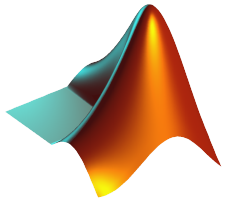
\includegraphics[width=2.5cm]{res/matlab.png}}
    \end{column}
    
    \begin{column}{.333\linewidth}
    Mathematica:\\
    \vspace {1cm}
    {
\includegraphics[width=2.5cm]{res/mat.png}}
    \end{column}
    
    \begin{column}{.333\linewidth}
    Integration with Steps:\\
    \vspace {1cm}
    {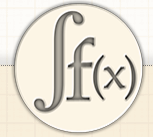
\includegraphics[width=2.5cm]{res/intc.png}}
    \scriptsize https://www.integral-calculator.com/\normalsize
    \end{column}
    
    \end{columns}
\end{frame}

\begin{frame}{About This Slide}
    You had better understand the contents on green slides. They are relatively fundamental.
\end{frame}
\colortheme{blue!50!black}
\begin{frame}{About This Slide}
    The content shown on blue slides may be relatively hard, but may contribute to getting high marks in the exams more or less. Do not worry when you cannot handle it.
\end{frame}
\colortheme{pink!100!black}
\begin{frame}{About This Slide}
    Those on pink slides are just some interesting problems and crazy thoughts. Maybe they are of little application in exams, but they are quite interesting.
\end{frame}
\colortheme{green!30!black}








% \section{Functions}

% \begin{frame}
%     \frametitle{Definitions \& Properties}
%     \framesubtitle{Basic definitions}
% Three essential factors of a function:
%         \begin{itemize}
%             \item Domain: $D$\\A set containing the action objects of correspondence rule.
% \item Correspondence Rule
%             \item Range: $E$\\ A set of all images corresponding to all elements in the domain under a certain correspondence rule.
%         \end{itemize}
%    \begin{block}{Definition}
%         A \textbf{function} $f$ is a rule that assigns to \alert{each element} $x$ in a set $D$ exactly one element, called $f(x)$, in a set $E$.
%     \end{block}
% \begin{block}{The Vertical Line Test}
%         A curve in the $xy$-plane is the graph of a function of $x$ \alert{iff} (if and only if) no vertical line intersects the curve more than once.
%     \end{block}
% \end{frame}

% \begin{frame}
% \frametitle{Definitions \& Properties}
%     \framesubtitle{Representation of Functions}
% There are four ways to represent a function:
%         \begin{enumerate}
%             \item Verbally (by a description in words)
%             \item Numerically (by a table of values)
%             \item Visually (by a graph)
%             \item Algebraically (by an explicit formula)
%         \end{enumerate}
% \end{frame}

% \begin{frame}
% \frametitle{Definitions \& Properties}
% \framesubtitle{Basic Properties}
%     \begin{block}{Symmetry}
%         \begin{itemize}
%             \item Even function: $f(-x)=f(x)$
%             \item Odd function: $f(-x)=-f(x)$
%         \end{itemize}
% Tip: Give priority to whether the domain \textit{D} of the function is symmetrical.
%     \end{block}
%     \begin{block}{Increasing \& Decreasing property}
%     A function $f$ is called (strictly) \textbf{increasing} on an interval $I$ if
% $$
% f\left(x_{1}\right)<f\left(x_{2}\right) \quad \text { whenever } x_{1}<x_{2} \text { in } I
% $$
% A function $f$ is called (strictly) \textbf{decreasing} on an interval $I$ if
% $$
% f\left(x_{1}\right)>f\left(x_{2}\right) \quad \text { whenever } x_{1}<x_{2} \text { in } I
% $$
%     \end{block}
% \end{frame}
% \begin{frame}{Basic function types}
%     \begin{block}{Linear function}
%         The graph of the function is a line:
%         \begin{center}
%             $y=f(x)=mx+b$
%         \end{center}
%        $m$ is the slope of the line and $b$ is the y-intercept.
%     \end{block}

%     \begin{block}{Polynomials}
%         A function $P$ is called a \textbf{polynomial} if
%         \begin{center}
%             $P(x)=\Sigma_{i=0}^n a_ix^i$
%         \end{center}
%        $a_i$ are \textbf{coefficients} and $n$ is the \textbf{degree} of the polynomial if $a_n\neq0$.
%     \end{block}
%     \begin{block}{Quadratic function}
%         A polynomial of degree 2 is of the form $P(x)=ax^2+bx+c$ and is called a \textbf{quadratic function}.
%     \end{block}
    
% \end{frame}

% \begin{frame}{Basic function types}
%     \begin{block}{Power function}
%         A function of the form $f(x)=x^a$ is called a \textbf{power function}, where $a$ is a constant. Consider an arbitary positive integer $n$:
%         \begin{itemize}
%             \item $a=n$:\\
%                 \begin{center}
%                     $y=x$: line \qquad $y=x^2$: parabola
%                 \end{center}
%             \item $a=\frac{1}{n}$: \textbf{root function}\\
%             \item $a=-1$: \textbf{reciprocal function}
%         \end{itemize}
%     \end{block}
%     \begin{block}{Ratio function}
%         A \textbf{Ratio function} $f$ is a ratio of two polynomials:
%         \begin{center}
%             $f(x)=\frac{P(x)}{Q(x)}$
%         \end{center}
%         The domain consists of all values of $x$ such that $Q(x)\neq 0$.
%     \end{block}
% \end{frame}

% \begin{frame}{Basic function types}
%     \begin{block}{Trigonometric function}
%         \begin{center}
%             $\sin (x+2\pi)=\sin x\qquad \cos (x+2\pi)=\cos x\qquad $
%             $\tan (x+\pi)=\tan x$
%         \end{center}
%     \end{block}
%     \begin{block}{Exponential function}
%         The \textbf{exponential functions} are the functions of the form $f(x) = a^x$, where the base a is a positive constant.
%     \end{block}
%     \begin{block}{Logarithmic function}
%         The \textbf{logarithmic functions} $f(x) = \log_ax$, where the base $a$ is a positive constant, are the inverse functions of the exponential functions. 
%     \end{block}
%     Think about the question:\\
%     What condition does $a$ meet when the exponential function increases in its domain? What about the logarithmic function?
% \end{frame}

% \begin{frame}{How to draw a function}
%     \begin{itemize}
%         \item You can simply trace the dots for simple functions.
%         \item You may also try to use software:\\
%             %\begin{center}
%                 https://www.geogebra.org\\
%                 https://www.desmos.com
%             %\end{center}
%     \end{itemize}
% \end{frame}
% \begin{frame}{Special Functions}
%     \begin{block}{Dirichlet Function}
    
% $$
% 1_{\mathbb{Q}}(x)= \begin{cases}1 & x \in \mathbb{Q} \\ 0 & x \notin \mathbb{Q}\end{cases}
% $$
%     \end{block}
% \end{frame}

% \begin{frame}{Special Functions}
%     \begin{block}{Impulse Function}
    
% $$
% \delta(t)= \begin{cases}\infty & t=0 \\ 0 & t \neq 0\end{cases}
% $$
%     \end{block}
%     \begin{block}{Step Function}
% $$
% H[n]= \begin{cases}0, & n<0 \\ 1, & n \geq 0\end{cases}
% $$
%     \end{block}
%     \begin{block}{Ramp Function}
% $$
% R(x):= \begin{cases}x, & x \geq 0 \\ 0, & x<0\end{cases}
% $$
%     \end{block}
% \end{frame}

% \begin{frame}{Special Functions}
%     \begin{block}{Hyperbolic Function}

% $$
% \sinh (x)=\frac{e^{x}-e^{-x}}{2}, \cosh (x)=\frac{e^{x}+e^{-x}}{2}, \tanh (x)=\frac{\sinh (x)}{\cosh (x)}
% $$
% %For more detail, see in textbook section $3.9$ and exercise.
%     \end{block}
%     \begin{block}{Inverse trigonometric function}

% $$
% \begin{aligned}
% &\arcsin (x), \arccos (x), \arctan (x) \\
% &\operatorname{arsinh}(x)=\ln \left(x+\sqrt{x^{2}+1}\right)\\ &\operatorname{arcosh}(x)=\ln \left(x+\sqrt{x^{2}-1}\right)\\ &\operatorname{artanh}(x)=\frac{1}{2} \ln \left(\frac{1+x}{1-x}\right)
% \end{aligned}
% $$
%     \end{block}
% \end{frame}
% \begin{frame}{Function Transformation}
%     \begin{block}{Vertical and Horizontal Shifts, suppose $c>0$}
%     $y=f(x)+c$, shift the graph of $y=f(x)$ a distance $c$ units upward\\ $y=f(x)-c$, shift the graph of $y=f(x)$ a distance $c$ units downward\\ $y=f(x-c)$, shift the graph of $y=f(x)$ a distance $c$ units to the right\\ $y=f(x+c)$, shift the graph of $y=f(x)$ a distance $c$ units to the left\\
%     \end{block}
%     \begin{block}{Vertical and Horizontal Stretching and Reflecting, suppose $c>1$}
%     $y=c f(x)$, stretch the graph of $y=f(x)$ vertically by a factor of $c$\\ $y=(1 / c) f(x)$, shrink the graph of $y=f(x)$ vertically by a factor of $c$\\
%     $y=f(c x)$, shrink the graph of $y=f(x)$ horizontally by a factor of $c$\\ $y=f(x / c)$, stretch the graph of $y=f(x)$ horizontally by a factor of $c$\\
%     $y=-f(x)$, reflect the graph of $y=f(x)$ about the $x$-axis\\ $y=f(-x)$, reflect the graph of $y=f(x)$ about the $y$-axis
%     \end{block}
% \end{frame}

% \begin{frame}{Function Combination}
%     \begin{block}{Definition}
%         Given two functions $f$ and $g$, the \textbf{composite function} $f \circ g$ (also called the \textbf{composition} of $f$ and $g$ ) is defined by
%         \begin{equation*}
%             (f \circ g)(x)=f(g(x))
%         \end{equation*}
%     \end{block}
%     \bigskip
%     It is possible to take the composition of three or more functions. For instance, the composite function $f \circ g \circ h$ is found by first applying $h$, then $g$, and then $f$ as follows:
%     $$
%     (f \circ g \circ h)(x)=f(g(h(x)))
%     $$
% \end{frame}

% \begin{frame}{Exercise 1}
%     \textit{Skip it if you find the exercise quite simple.}\\
% \bigskip
%     Find the domain of these functions:
% \begin{enumerate}
%     \item $h(x)=\frac{1}{\sqrt[4]{x^{2}-5 x}}$\\
%     \item $f(u)=\frac{u+1}{1+\frac{1}{u+1}}$\\
%     \item $F(p)=\sqrt{2-\sqrt{p}}$
% \end{enumerate}
% \end{frame}

% \begin{frame}
% \frametitle{Exercise 1}
% \framesubtitle{Conclusions}
%     \begin{block}{How to solve this kind of questions}
%         \begin{itemize}
%             \item The denominator in the fractional function cannot be zero
%             \item The quantity in the even root formula cannot take a negative value, that is, it should be greater than or equal to zero
%             \item The antilogarithm of the logarithm cannot be negative and zero, that is, it must take a positive value
%             \item The domain of the function $y=\arcsin x, y=\arccos x$ is $-1 \leqslant x \leqslant 1$
%             \item $y=\tan x$ , $x \neq k \pi+\pi / 2, y=\cot x$ , $x \neq k \pi$, $k$ is integer
%         \end{itemize}
%     \end{block}
% \end{frame}

% \begin{frame}{Exercise 2}
%     \begin{block}{Prove or Disprove}
%         \begin{itemize}
%             \item If $f$ and $g$ are both even functions, is $f+g$ even? If $f$ and $g$ are both odd functions, is $f+g$ odd? What if $f$ is even and $g$ is odd? Justify your answers.
%             \item If $f$ and $g$ are both even functions, is the product $f g$ even? If $f$ and $g$ are both odd functions, is $f g$ odd? What if $f$ is even and $g$ is odd? Justify your answers.
%         \end{itemize}
%     \end{block}
% \end{frame}

% \begin{frame}{Exercise 3}
%     \begin{block}{Graph the functions step by step}
%     (1)$y=1-2 \sqrt{x+3}$\\
%     (2)$y=|\cos \pi x|$
%     \end{block}
% \end{frame}


% \begin{frame}{Exercise 4}
%     \begin{block}{Find the function (a) $f \circ g$, (b) $g \circ f$, (c) $f \circ f$, and (d) $g \circ g$ and their domains.}
%     $f(x)=\frac{x}{1+x}, \quad g(x)=\sin 2 x$\\
%     \end{block}
% \end{frame}

% \begin{frame}{Exercise 5}
%     Find $f \circ g\circ h$:\\
% \begin{itemize}
%     \item $f(x)=\tan x$
%  \item $g(x)=\frac{x}{x-1}$
% \item $h(x)=\sqrt[3]{x}$
% \end{itemize}
% (It is unnecessary to find the domain of this composite function in this exercise!)
% \end{frame}

% \begin{frame}{Exercise 6}
%     \begin{block}{Composite Function}
% \begin{enumerate}
%     \item If $g(x)=2 x+1$ and $h(x)=4 x^{2}+4 x+7$, find a function $f$ such that $f \circ g=h$. \\(Think about what operations you would have to perform on the formula for $g$ to end up with the formula for $h$.)\\
% \item If $f(x)=3 x+5$ and $h(x)=3 x^{2}+3 x+2$, find a function $g$ such that $f \circ g=h$.\\
% \end{enumerate}
%     \end{block}
% \end{frame}

% \begin{frame}{References}
% 	[1] Huang, Yucheng. VV156\_RC1\_updated.pdf. 2021.\\
% 	\bigskip
% 	[2] Cai, Runze. Chapter01.pdf. 2021.\\
% 	\bigskip
% 	[3] Zhou,Yishen.RC1. 2022.
% \end{frame}

% \begin{frame}{Exercise Answer 1-2}
%     \begin{enumerate}
%         \item $x^2-5x>0$ $\Rightarrow$ $x\in (-\infty,0)\cup (5,\infty)$
%         \item $1+\frac{1}{u+1}\neq0,u+1\neq0$ $\Rightarrow$ $u\in (\infty,-2)\cup(-2,-1)\cup (-1,\infty)$
%         \item $p\geq0,2-\sqrt{q}\geq0$ $\Rightarrow$ $p\in [0,4]$
%     \end{enumerate}
%     \vspace{1.5cm}
%     \begin{itemize}
%         \item Yes. Yes. Not necessarily.
%         \item Yes. No.(fg is Even) fg is Odd.
%     \end{itemize}
% \end{frame}


% \begin{frame}{Exercise Answer 3}
% \begin{center}
%     (1)\\
%     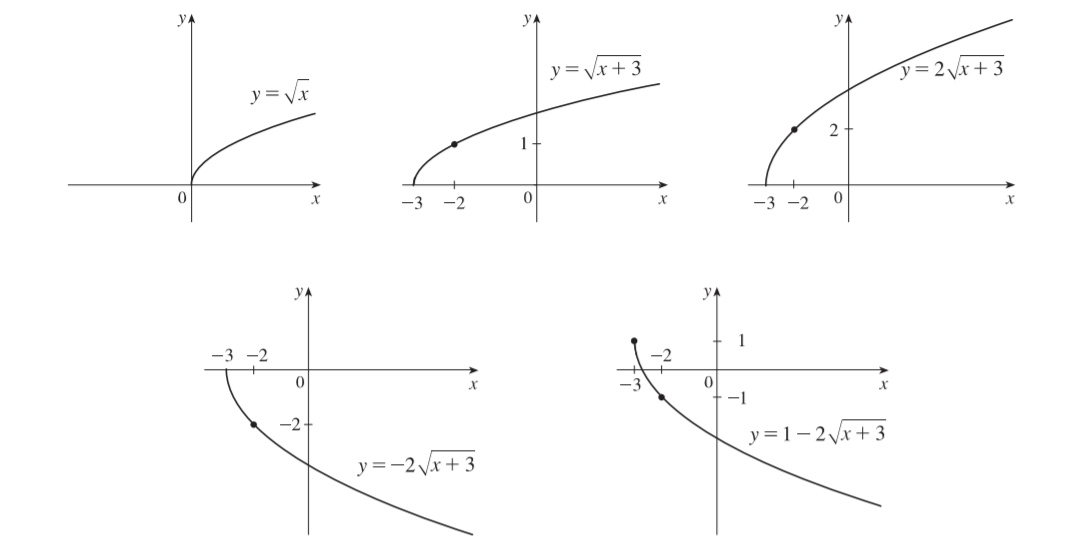
\includegraphics[width =8cm]{res/514.png}\\
%     \vspace{1cm}
%     (2)\\
%     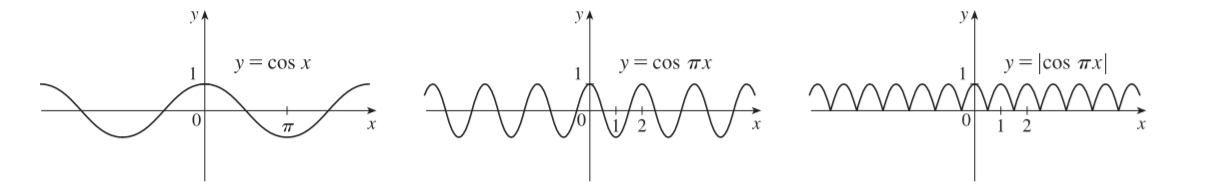
\includegraphics[width =8cm]{res/114.png}
% \end{center}
% \end{frame}

% \begin{frame}{Exercise Answer 4-5}
%     (a) $f\circ g(x)=\frac{sin 2x}{1+sin 2x}$. Domain: $x\in\{x|x\neq k\pi-\frac{\pi}{4},k\in\mathbb{B}\}$\\
%     (b) $g\circ f(x)=sin(\frac{2x}{1+x})$. Domain: $x\in (\infty,-1)\cup(-1,\infty)$\\
%     (c) $f\circ f(x)=\frac{x}{1+2x}(x\neq-1)$. Domain:$x\in (\infty,-1)\cup(-1,-\frac{1}{2})\cup (-\frac{1}{2},\infty)$\\
%     (d) $g\circ g(x)=sin(2sin(2x))$. Domain:$x\in\mathbb{R}$\\
%     \vspace{1.5cm}
%     $tan(\frac{\sqrt[3]{x}}{\sqrt[3]{x}-1})$
% \end{frame}

% \begin{frame}{Exercise Answer 6}
%     \begin{enumerate}
%         \item $x=\frac{g(x)-1}{2}$.\\
%         Plug into h(x), $h(x)=4(\frac{g(x)-1}{2})^2+4(\frac{g(x)-1}{2})+7=g^2(x)+6$.\\
%         Also, $h(x)=f(g(x))$.\\
%         Therefore, $f(x)=x^2-6$
%         \item $3g(x)+5=h(x)$, $g(x)=x^2+x-1$
%     \end{enumerate}
% \end{frame}

% \section{Limits}
%     \begin{frame}
% 		\frametitle{"Rough" Definition of a Limit}
% 		Suppose $f(x)$ is defined when $x$ is near the number $a$. (This means that $f$ is defined on some open interval that contains $a$, \alert{except possibly} at $a$ itself.)\\
% 		Then we write
% 		\begin{center}
% 			$\lim\limits_{\textit{x} \to a}f(x) = L$
% 		\end{center}
% 		and say
% 		\begin{center}
% 			"the limit if $f(x)$, as $x$ approaches $a$, equals $L$"
% 		\end{center}
% 		if we can make the values of $f(x)$ arbitrarily close to $L$ (as close to $L$ as we like) by taking $x$ to be \alert{sufficiently close to} $a$ (on either side of $a$) but \alert{not equal to} $a$.
% 	\end{frame}
% 	\begin{frame}
% 		\frametitle{One-sided Limits}
% 		Considering a function called \textit{Heaviside Function}\\
% 		\begin{center}
% 			\begin{equation}
% 				H(t)=
% 				\begin{cases}
% 					0 & t<0\\
% 					1 & t \geq 0
% 				\end{cases}
% 			\end{equation}
% 		\end{center}
% 		Does $\lim\limits_{\textit{t} \to 0}H(t)$ exists?
% 	\end{frame}
% 	\begin{frame}
% 		\frametitle{One-sided Limits}
% 		We write
% 		\begin{center}
% 			$\lim\limits_{\textit{x} \to a^{-}}f(x) = L$
% 		\end{center}
% 		and say the left-hand limit of $f(x)$ as $x$ approaches $a$ is equal to $L$ if we can make the values of $f(x)$ arbitrarily close to $L$ by taking $x$ to be \alert{sufficiently close to} $a$ and $x$ less than $a$.\\
% 		\bigskip
% 		When calculating $\lim\limits_{\textit{x} \to a^{-}}f(x)$, we consider only $x < a$.\\
% 		\bigskip
% 		Similarly, we can get the right-hand limit of $f(x)$ as $x$ approaches $a$.
% 	\end{frame}
% 	\begin{frame}
% 		\frametitle{One-sided Limits}
% 		When does $\lim\limits_{\textit{x} \to a}f(x)$ exists?\\
% 		\bigskip
% 		\begin{center}
% 			$\lim\limits_{\textit{x} \to a}f(x) = L$\\
% 			\bigskip
% 			\alert{if and only if}\\
% 			\bigskip
% 			$\lim\limits_{\textit{x} \to a^{-}}f(x) = L$ and $\lim\limits_{\textit{x} \to a^{+}}f(x) = L$
% 		\end{center}
% 		Can we directly regard $L$ as $f(a)$?
% 	\end{frame}
% 	\begin{frame}

% 		\frametitle{Infinite Limits}
% 		Let $f$ be a function defined on both sides of $a$, \alert{except possibly} at $a$ itself. Then
% 		\begin{center}
% 			$\lim\limits_{\textit{x} \to a}f(x) = \infty$
% 		\end{center}
% 		means that the values of $f(x)$ can be made arbitrarily large (as large as we please) by taking $x$ \alert{sufficiently close to} $a$, but \alert{not equal to} $a$.\\
		
% 		Let $f$ be a function defined on both sides of $a$, \alert{except possibly} at $a$ itself. Then
% 		\begin{center}
% 			$\lim\limits_{\textit{x} \to a}f(x) = -\infty$
% 		\end{center}
% 		means that the values of $f(x)$ can be made arbitrarily large negative by taking $x$ \alert{sufficiently close to} $a$, but \alert{not equal to} $a$.
% 	\end{frame}
% 	\begin{frame}
% 		\frametitle{Infinite Limits}
% 		\alert{Warning:}\\
% 		$\lim\limits_{\textit{x} \to a}f(x) = (-)\infty$ does not mean that we are regarding $(-)\infty$ as a number. Nor does it mean that the limit exists!
% 	\end{frame}
% 	\begin{frame}
% 		\frametitle{Limits at Infinity}
% 		\begin{enumerate}
% 			\item Let $f$ be a function defined on some interval ($a$, $\infty$). Then
% 			\begin{center}
% 				$\lim\limits_{\textit{x} \to \infty}f(x) = L$
% 			\end{center}
% 			means that the values of $f(x)$ can be made arbitrarily close to $L$ by taking $x$ sufficiently large.
% 		\item Let $f$ be a function defined on some interval ($-\infty$, $a$). Then
% 			\begin{center}
% 				$\lim\limits_{\textit{x} \to -\infty}f(x) = L$
% 			\end{center}
% 			means that the values of $f(x)$ can be made arbitrarily close to $L$ by taking $x$ sufficiently large negative.
% 		\end{enumerate}
% 	\end{frame}
% 	\begin{frame}
% 		\frametitle{Infinite Limits at Infinity}
% 		\begin{enumerate}
% 			\item $\lim\limits_{\textit{x} \to \infty}f(x) = \infty$
% 			\item $\lim\limits_{\textit{x} \to \infty}f(x) = -\infty$
% 			\item $\lim\limits_{\textit{x} \to -\infty}f(x) = \infty$
% 			\item $\lim\limits_{\textit{x} \to -\infty}f(x) = -\infty$
% 		\end{enumerate}
% 	\end{frame}
% 	\begin{frame}
% 		\frametitle{The Limit Laws}
% 		Five basic laws:\\
% 		Suppose that $c$ is a constant and the limits
% 		\begin{center}
% 			$\lim\limits_{\textit{x} \to a}f(x)$ and $\lim\limits_{\textit{x} \to a}g(x)$
% 		\end{center}
% 		exists. Then
% 		\begin{enumerate}
% 			\item $\lim\limits_{\textit{x} \to a}[f(x)+g(x)] = \lim\limits_{\textit{x} \to a}f(x) + \lim\limits_{\textit{x} \to a}g(x)$
% 			\item $\lim\limits_{\textit{x} \to a}[f(x)-g(x)] = \lim\limits_{\textit{x} \to a}f(x) - \lim\limits_{\textit{x} \to a}g(x)$
% 			\item $\lim\limits_{\textit{x} \to a}[cf(x)] = c\lim\limits_{\textit{x} \to a}f(x)$
% 			\item $\lim\limits_{\textit{x} \to a}[f(x)g(x)] = \lim\limits_{\textit{x} \to a}f(x) \cdot \lim\limits_{\textit{x} \to a}g(x)$
% 			\item $\lim\limits_{\textit{x} \to a}\dfrac{f(x)}{g(x)} = \dfrac{\lim\limits_{\textit{x} \to a}f(x)}{\lim\limits_{\textit{x} \to a}g(x)}$\ \ \  \alert{(if $\lim\limits_{\textit{x} \to a}g(x) \neq 0$)}
% 		\end{enumerate}
% 	\end{frame}
% 	\begin{frame}
% 		\frametitle{The Limit Laws}
% 		Another six laws:
% 		\begin{enumerate}
% 			\item $\lim\limits_{\textit{x} \to a}[f(x)]^{n} = [\lim\limits_{\textit{x} \to a}f(x)]^{n}$ (where $n$ is a positive integer)
% 			\item $\lim\limits_{\textit{x} \to a}c = c$
% 			\item $\lim\limits_{\textit{x} \to a}x = a$
% 			\item $\lim\limits_{\textit{x} \to a}x^{n} = a^{n}$ (where $n$ is a positive integer)
% 			\item $\lim\limits_{\textit{x} \to a}\sqrt[n]{x} = \sqrt[n]{a}$ (where $n$ is a positive integer)\\
% 				\alert{if $n$ is even, we assume that $a > 0$}
% 			\item $\lim\limits_{\textit{x} \to a}\sqrt[n]{f(x)} = \sqrt[n]{\lim\limits_{\textit{x} \to a}f(x)}$ (where $n$ is a positive integer)\\
% 				\alert{if $n$ is even, we assume that $\lim\limits_{\textit{x} \to a}f(x) > 0$}
% 		\end{enumerate} 
% 	\end{frame}
% 	\begin{frame}
% 		\frametitle{The Limit Laws}
% 		\alert{Warning:}\\
% 		The Limit Laws can't be applied to infinite limits because $(-)\infty$ is not a number!
% 	\end{frame}
% 	\begin{frame}
% 		\frametitle{The Limit Laws}
% 		Two additional properties of limits:
% 		\begin{enumerate}
% 				\item if $f(x) \leq g(x)$ when $x$ is near $a$ (\alert{except possibly} at $a$) and the limits of $f$ and $g$ both exists as $x$ approaches $a$, then
% 					\begin{center}
% 						$\lim\limits_{\textit{x} \to a}f(x) \leq \lim\limits_{\textit{x} \to a}g(x)$
% 					\end{center}
% 				\item \alert{(The Squeeze Theorem)} if $f(x) \leq g(x) \leq h(x)$ when $x$ is near $a$ (\alert{except possibly} at $a$) and
% 					\begin{center}
% 						$\lim\limits_{\textit{x} \to a}f(x) = \lim\limits_{\textit{x} \to a}h(x) = L$
% 					\end{center}
% 					then
% 					\begin{center}
% 						$\lim\limits_{\textit{x} \to a}g(x) = L$
% 					\end{center}
% 		\end{enumerate}
% 	\end{frame}

% 	\begin{frame}
% 		\frametitle{Two Important Limits}
% 		Be sure to keep these two limits in mind!
% 		\begin{enumerate}
% 			\item $\lim\limits_{\textit{x} \to 0}\dfrac{\sin{x}}{x} = 1$\\
% 				(How to prove it? Considering $\sin{x}$, $x$ and $\tan{x}$. Then, use the squeeze theorem.)
% 			\item $\lim\limits_{\textit{x} \to \infty}(1 + \dfrac{1}{x})^{x} = e = 2.718281828459045\cdots$
% 		\end{enumerate}
% 		\begin{columns}[c] % The "c" option specifies centered vertical alignment while the "t" option is used for top vertical alignment
% 			\begin{column}{0.5\textwidth} % Left column width
% 				\begin{figure}
% 					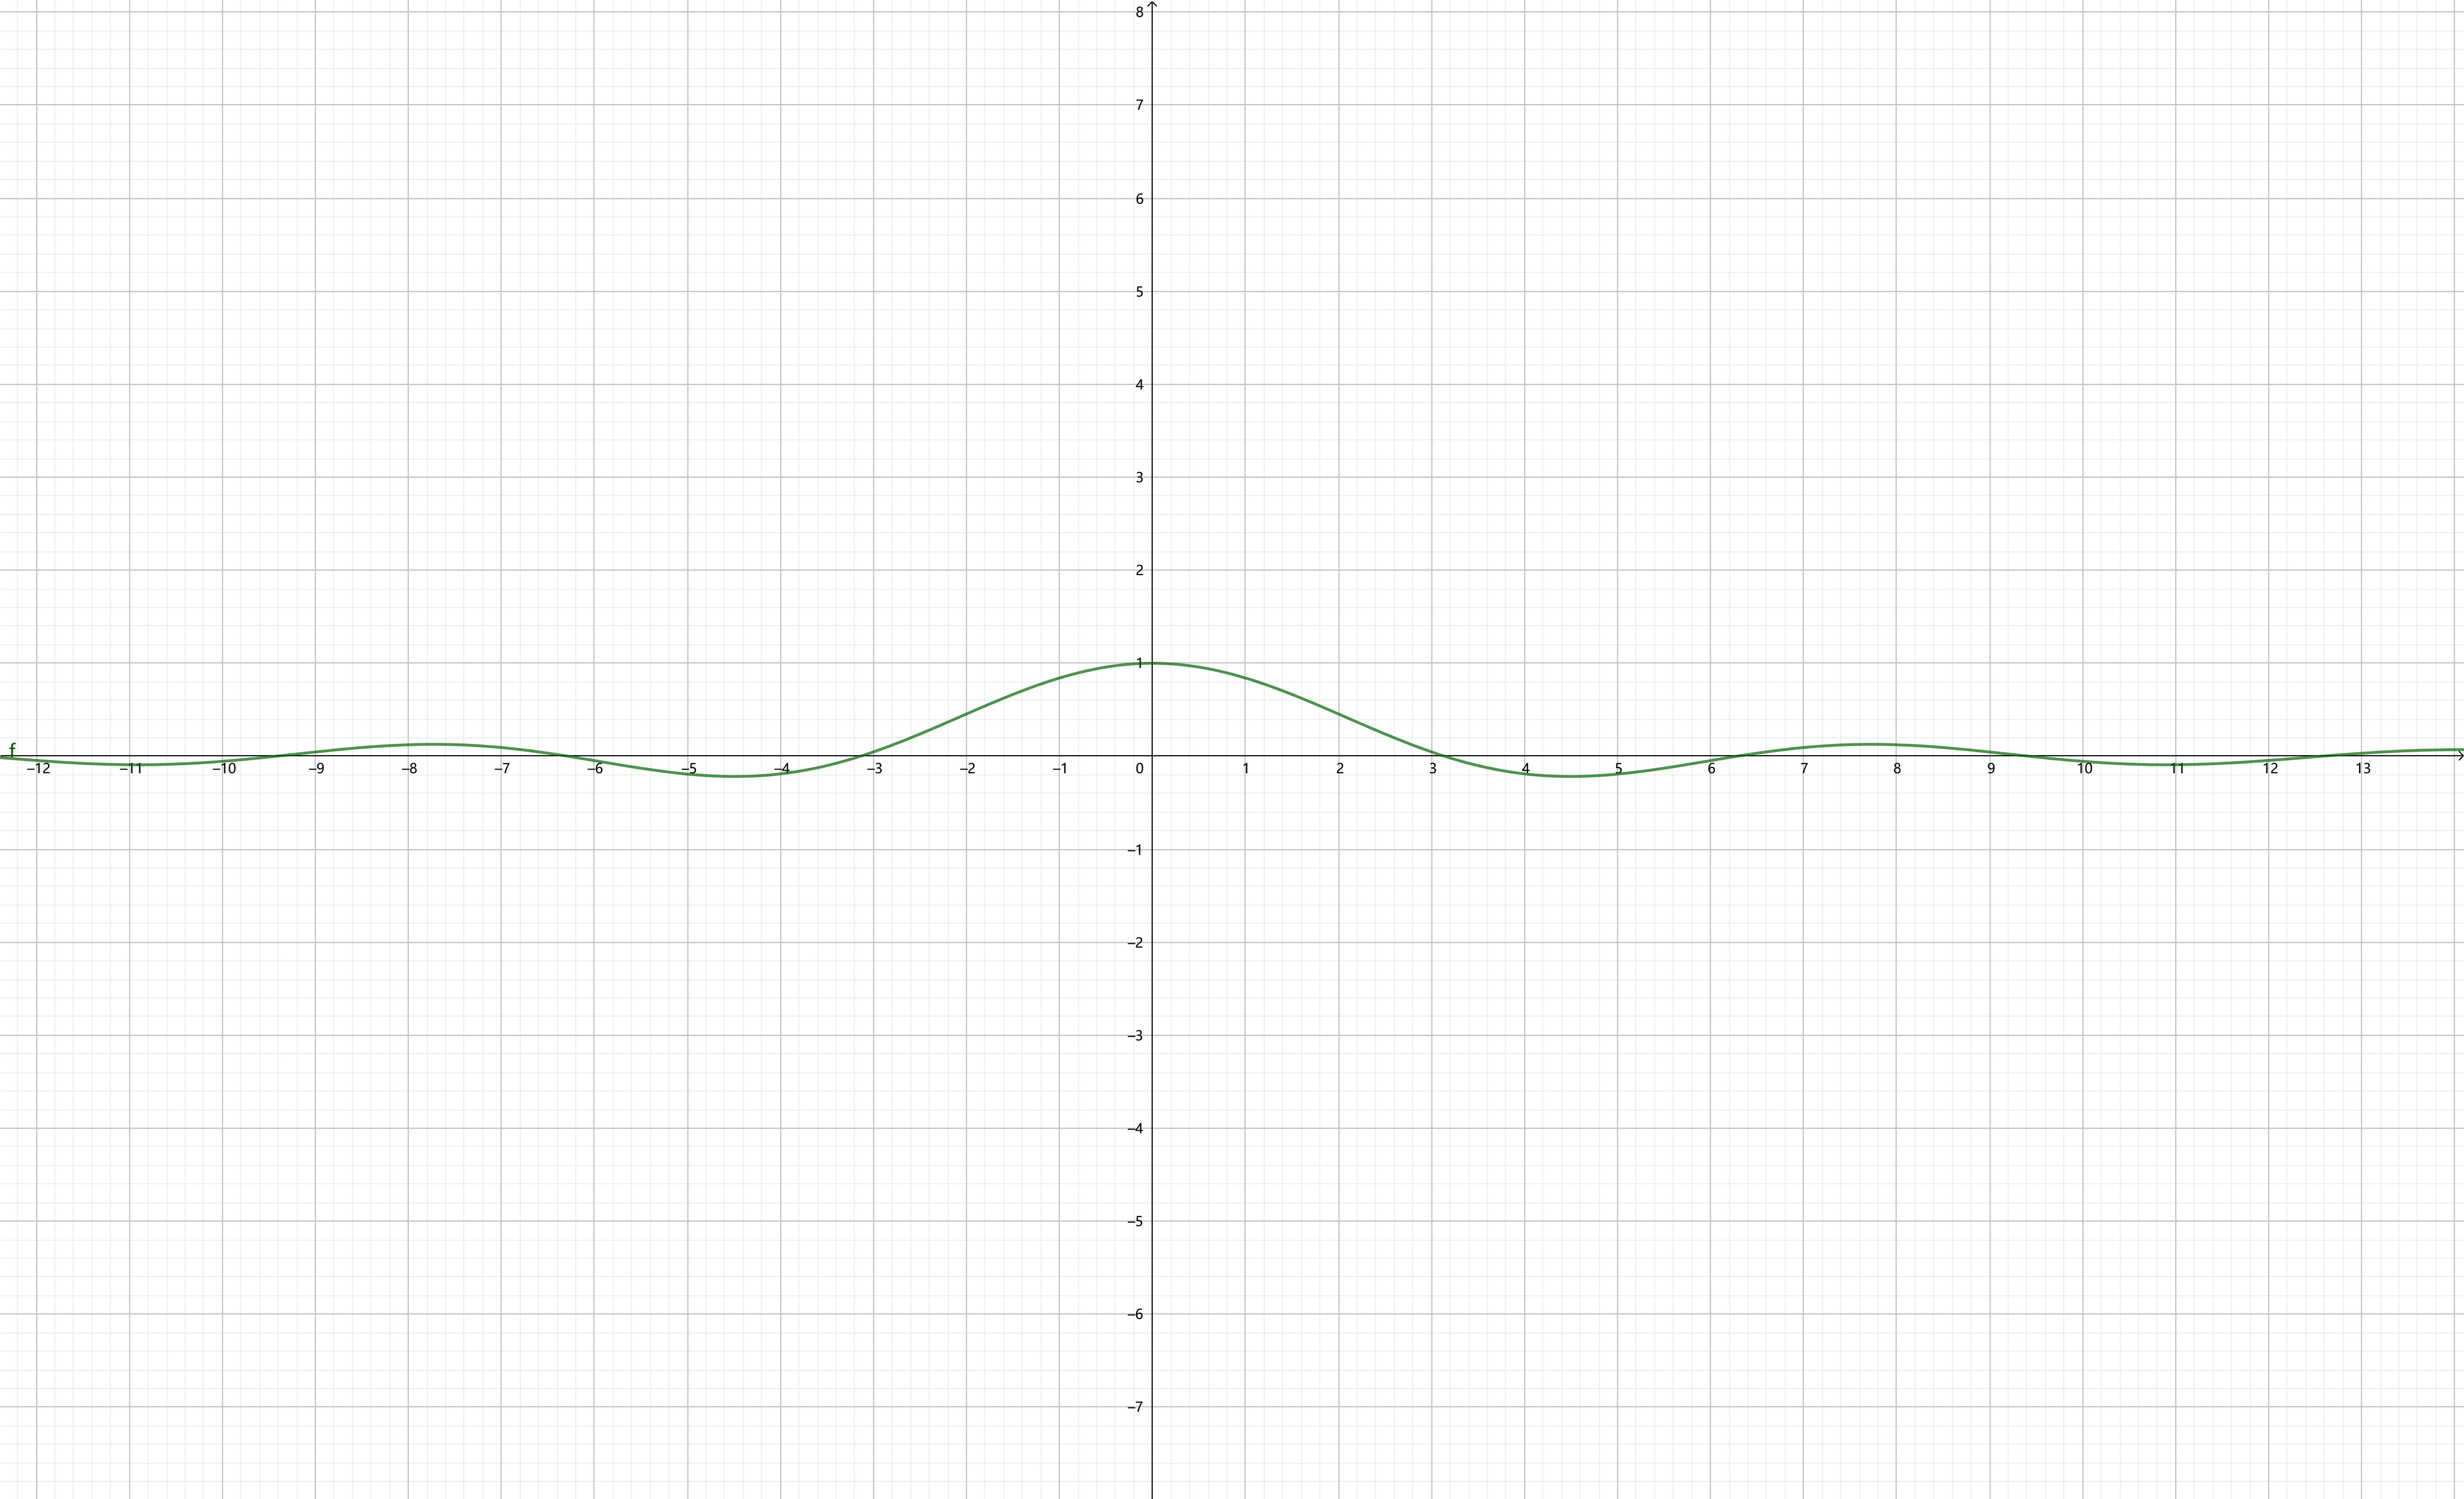
\includegraphics[width=1\linewidth]{bbb.jpg}
% 				\end{figure}
% 			\end{column}
% 			\begin{column}{0.5\textwidth} % Right column width
% 				\begin{figure}
% 					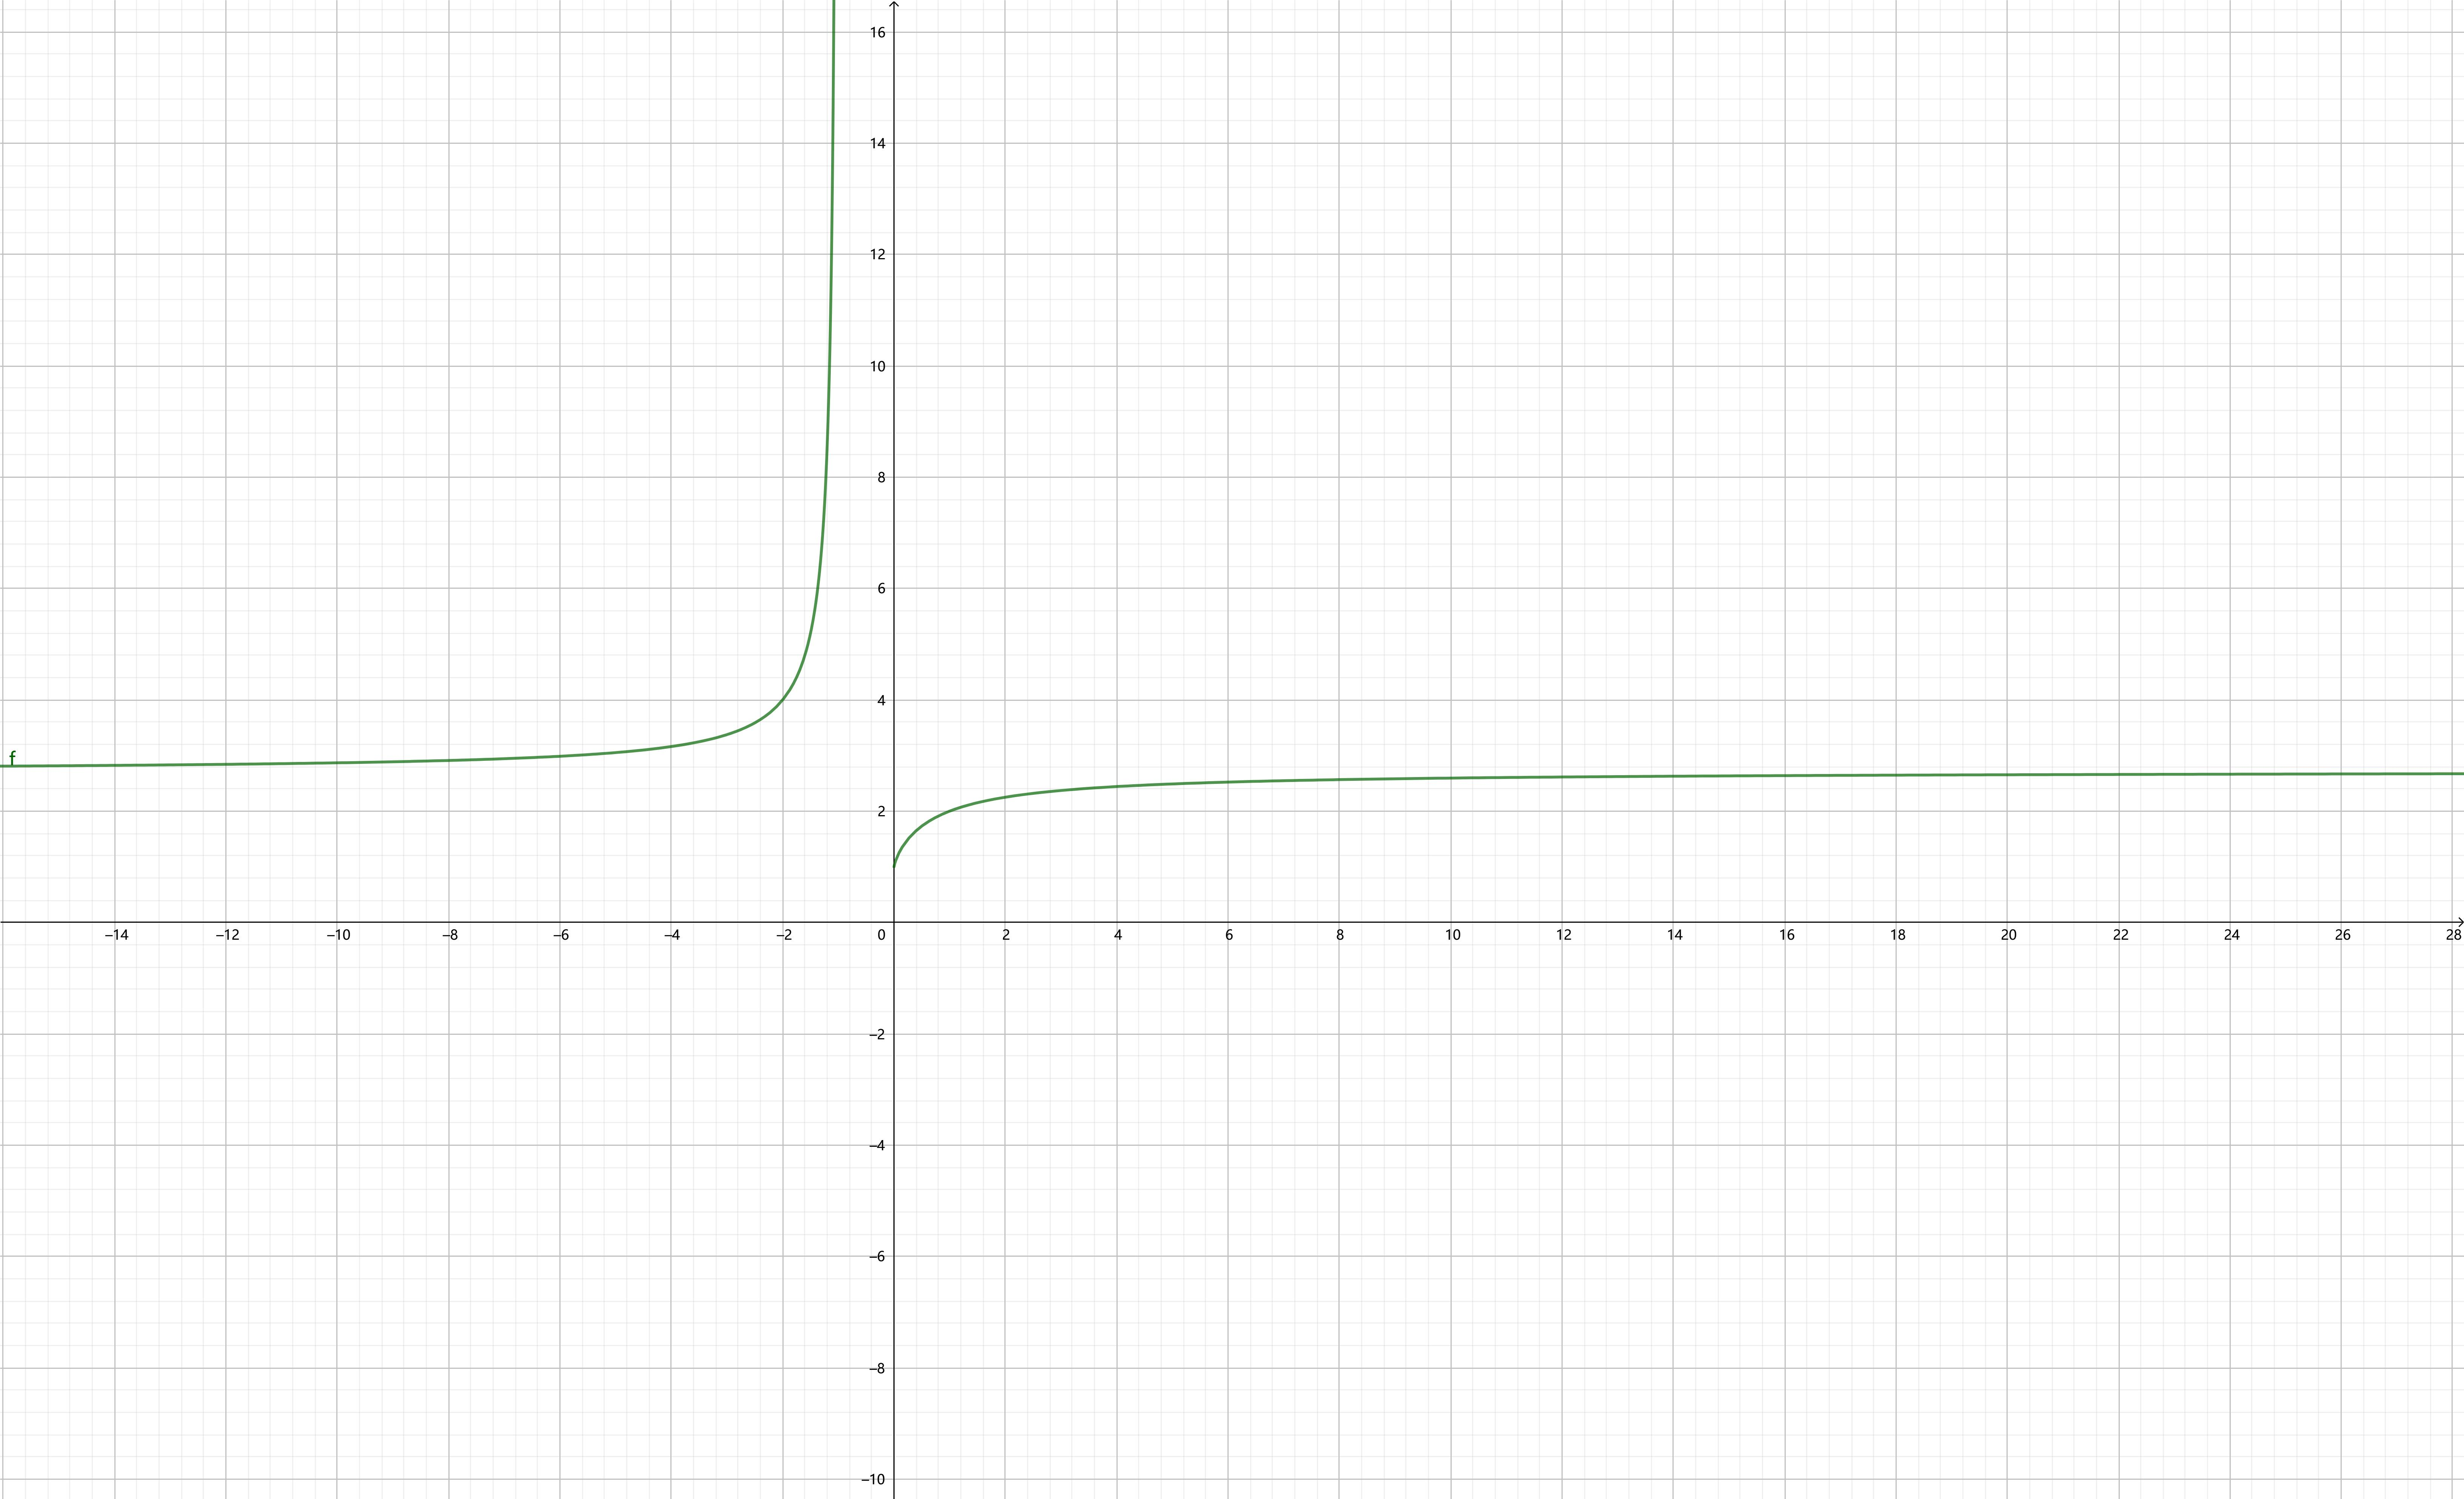
\includegraphics[width=1\linewidth]{aaa.jpg}
% 				\end{figure}
% 			\end{column}
% 	\end{columns}
% 	\end{frame}
	
%     \colortheme{blue!50!black}
    
% 	\begin{frame}
% 		\frametitle{The Precise Definition of a Limit}
% 		Let $f$ be a function defined on some open interval that contains the number $a$, \alert{except possibly} at $a$ itself. Then we say that the limit if $f(x)$ as $x$ approaches $a$ is $L$, and we write
% 		\begin{center}
% 				$\lim\limits_{\textit{x} \to a}f(x) = L$
% 		\end{center}
% 		if for \alert{every} number $\varepsilon > 0$, there is a number $\delta > 0$ such that
% 		\begin{center}
% 				if\ \ \ $0 < |x - a| < \delta$\ \ \ then\ \ \ $|f(x) - L| < \varepsilon$
% 		\end{center}
% 	\end{frame}
% 	\begin{frame}
% 		\frametitle{The Precise Definition of a Limit}
% 		Left-hand limits:
% 		\begin{center}
% 				$\lim\limits_{\textit{x} \to a^{-}}f(x) = L$
% 		\end{center}
% 		if for \alert{every} number $\varepsilon > 0$, there is a number $\delta > 0$ such that
% 		\begin{center}
% 				if\ \ \ $a - \delta < x < a$\ \ \ then\ \ \ $|f(x) - L| < \varepsilon$
% 		\end{center}
% 		Right-hand limits:
% 		\begin{center}
% 				$\lim\limits_{\textit{x} \to a^{+}}f(x) = L$
% 		\end{center}
% 		if for \alert{every} number $\varepsilon > 0$, there is a number $\delta > 0$ such that
% 		\begin{center}
% 				if\ \ \ $a < x < a + \delta$\ \ \ then\ \ \ $|f(x) - L| < \varepsilon$
% 		\end{center}
% 	\end{frame}
% 	\begin{frame}
% 		\frametitle{The Precise Definition of a Limit}
% 		Infinite limits:\\
% 		\begin{enumerate}
% 		\item Let $f$ be a function defined on some open interval that contains the number $a$, \alert{except possibly} at $a$ itself. Then
% 			\begin{center}
% 					$\lim\limits_{\textit{x} \to a}f(x) = \infty$
% 			\end{center}
% 			means that for \alert{every positive} number $M$, there is a number $\delta > 0$ such that
% 			\begin{center}
% 					if\ \ \ $0 < |x - a| < \delta$\ \ \ then\ \ \ $f(x) > M$
% 			\end{center}
% 		\item Let $f$ be a function defined on some open interval that contains the number $a$, \alert{except possibly} at $a$ itself. Then
% 			\begin{center}
% 					$\lim\limits_{\textit{x} \to a}f(x) = -\infty$
% 			\end{center}
% 			means that for \alert{every negative} number $N$, there is a number $\delta > 0$ such that
% 			\begin{center}
% 					if\ \ \ $0 < |x - a| < \delta$\ \ \ then\ \ \ $f(x) < N$
% 			\end{center}
% 		\end{enumerate}
% 	\end{frame}
% 	\begin{frame}
% 		\frametitle{The Precise Definition of a Limit}
% 		Limits at Infinity:\\
% 		\begin{enumerate}
% 		\item Let $f$ be a function defined on some interval ($a$, $\infty$). Then
% 			\begin{center}
% 				$\lim\limits_{\textit{x} \to \infty}f(x) = L$
% 			\end{center}
% 			means that for every $\varepsilon > 0$, there is a corresponding number $N$ such that
% 			\begin{center}
% 				if\ \ \ $x > N$\ \ \ then\ \ \ $|f(x) - L| < \varepsilon$
% 			\end{center}
% 		\item Let $f$ be a function defined on some interval ($-\infty$, $a$). Then
% 			\begin{center}
% 				$\lim\limits_{\textit{x} \to -\infty}f(x) = L$
% 			\end{center}
% 			means that for every $\varepsilon > 0$, there is a corresponding number $N$ such that
% 			\begin{center}
% 				if\ \ \ $x < N$\ \ \ then\ \ \ $|f(x) - L| < \varepsilon$
% 			\end{center}
% 	\end{enumerate}
% 	\end{frame}
    
%     \colortheme{green!30!black}

% 	\begin{frame}
% 		\frametitle{Exercise 1}
% 		Evaluate the following limits\\
% 		\begin{enumerate}
% 			\item $\lim\limits_{\textit{x} \to 0}\dfrac{4x^{3}-2x^{2}+x}{2x+3x^{2}}$
% 			\item $\lim\limits_{\textit{x} \to 0}\dfrac{\dfrac{1}{3+x}-\dfrac{1}{3}}{x}$
% 			\item $\lim\limits_{\textit{x} \to \infty}(1+\dfrac{1}{x})(2-\dfrac{1}{x^{2}})$
% 			\item $\lim\limits_{\textit{x} \to 0}\dfrac{-1+\sqrt[n]{x+1}}{x}$
			
% 		\end{enumerate}
% 	\end{frame}
% 	\colortheme{blue!50!black}
% 	\begin{frame}
% 		\frametitle{Exercise 2}
% 		Evaluate the following limits\\
% 		\begin{enumerate}
% 		    \item $\lim\limits_{\textit{x} \to -4}\dfrac{\sqrt{9+x^{2}}-5}{x+4}$
% 			\item $\lim\limits_{\textit{\alert{h}} \to 0}\dfrac{(x+h)^{3}-x^{3}}{h}$(What if $\lim\limits_{\textit{\alert{h}} \to 0}\dfrac{(x+h)^{n}-x^{n}}{h}$?)
% 			\item $\lim\limits_{\textit{x} \to 0}\dfrac{\sin{\omega x}}{x}$
% 			\item $\lim\limits_{\textit{x} \to \infty}(1-\dfrac{1}{x})^{kx}$\ \ \ ($k$ is a positive integer)
% 			\item $\lim\limits_{\textit{x} \to \dfrac{\pi}{2}}(\sin{x})^{\tan{x}}$
% 		\end{enumerate}
% 	\end{frame}
% 	\colortheme{green!30!black}
% 	\begin{frame}
% 		\frametitle{Conclusions}
% 		Some methods to calculate the limits:
% 		\begin{enumerate}
% 			\item Use those limit laws directly
% 			\item Exchange the order of functions and limit symbols based on the continuity of composite function. (Will be mentioned later)
% 			\item Do factorization, denominator rationalization or numerator rationalization.
% 			\item If a factor approaching zero is find in the denominator, try to eliminate it.
% 			\item Translate the formula into the form of "two important limits"
% 			\item \alert{The method to solve those formulas having the form of $u(x)^{v(x)}$ will be discussed at a deeper level after the differentiation and l'Hôpital's rule are taught.}
% 		\end{enumerate}
% 	\end{frame}
% 	\begin{frame}{Exercise Answer 1}
% 	    \begin{enumerate}
	    
% 			\item $\lim\limits_{\textit{x} \to 0}\dfrac{4x^{3}-2x^{2}+x}{2x+3x^{2}}=\lim\limits_{\textit{x} \to 0}\dfrac{4x^{2}-2x+1}{2+3x}$=0.5
% 			\item $\lim\limits_{\textit{x} \to 0}\dfrac{\dfrac{1}{3+x}-\dfrac{1}{3}}{x}=\lim\limits_{\textit{x} \to 0}\dfrac{3-3-x}{3x(3+x)}=\lim\limits_{\textit{x} \to 0}\dfrac{-1}{3(3+x)}=-\dfrac{1}{9}$
% 			\item $\lim\limits_{\textit{x} \to \infty}(1+\dfrac{1}{x})(2-\dfrac{1}{x^{2}})=\lim\limits_{\textit{x} \to \infty}(1+\dfrac{1}{x})\cdot\lim\limits_{\textit{x} \to \infty}(2-\dfrac{1}{x^{2}})=1\cdot2=2$
% 			\item Let $t^{n}-1:=x$, $\lim\limits_{\textit{x} \to 0}\dfrac{-1+\sqrt[n]{x+1}}{x}=\lim\limits_{\textit{t} \to 1}\dfrac{t-1}{t^{n}-1}=\lim\limits_{\textit{t} \to 1}\dfrac{1}{1+t+t^2+\cdots+t^{n-1}}=\dfrac{1}{n}$
% 		\end{enumerate}
% 	\end{frame}
% 	\colortheme{blue!50!black}
% 	\begin{frame}{Exercise Answer 2}
% 	    \small
% 	    \begin{enumerate}
% 		    \item $\lim\limits_{\textit{x} \to -4}\dfrac{\sqrt{9+x^{2}}-5}{x+4}=\lim\limits_{\textit{x} \to -4}\dfrac{x-4}{\sqrt{9+x^{2}}+5}=-\dfrac{4}{5}$
% 			\item $\lim\limits_{\textit{\alert{h}} \to 0}\dfrac{(x+h)^{n}-x^{n}}{h}=\lim\limits_{\textit{\alert{h}} \to 0}nx^{n-1}+h\cdot(\cdots)=nx^{n-1}$
% 			\item $\lim\limits_{\textit{x} \to 0}\dfrac{\sin{\omega x}}{x}=\omega\cdot\lim\limits_{\textit{x} \to 0}\dfrac{\sin{\omega x}}{\omega x}=\omega$
% 			\item $\lim\limits_{\textit{x} \to \infty}(1-\dfrac{1}{x})^{kx}=\lim\limits_{\textit{x} \to \infty}(1+\dfrac{1}{-x})^{(-x)(-k)}=e^{-k}$
% 			\item $\lim\limits_{\textit{x} \to \dfrac{\pi}{2}}(\sin{x})^{\tan{x}}=\lim\limits_{\textit{x} \to \dfrac{\pi}{2}}(1+(\sin{x}-1))^{\dfrac{1}{\sin{x}-1}\cdot(\sin{x}-1)\tan{x}}=e^{\lim\limits_{\textit{x} \to \dfrac{\pi}{2}}(\sin{x}-1)\tan{x}}=e^{\lim\limits_{\textit{x} \to \dfrac{\pi}{2}}\dfrac{(\sin{x}-1)\sin{x}}{\sqrt{1-\sin^2x}}}=e^{-\lim\limits_{\textit{x} \to \dfrac{\pi}{2}}\dfrac{\sqrt{1-\sin{x}}\sin{x}}{\sqrt{1+\sin x}}}=e^0=1$
% 		\end{enumerate}
% 		\normalsize
% 	\end{frame}
% 	\colortheme{green!30!black}
	
	

	
% 	\begin{frame}{References}
% 	    \frametitle{References}
% 		[1] Huang, Yucheng. VV156\_RC2.pdf. 2021.\\
% 		\bigskip
% 		[2] Cai, Runze. Chapter01.pdf. 2021.\\
% 		\bigskip
% 		[3] Department of mathematics, Tongji University. Advanced Mathematics (7th Edition). 2014.\\
% 		\bigskip
% 		[4] James Stewart. Calculus (7th Edition). 2014.\\
% 		\bigskip
% 		[5] Department of mathematics, Tongji University. Learning Guidance of Advanced Mathematics (7th Edition). 2014.\\
% 		\bigskip
% 		[6]Zhou,Yishen.RC2. 2022.
% 	\end{frame}
% \section{Continuity}
% \begin{frame}
% 		\frametitle{Definition of Continuity}
% 		A function $f$ is continuous at a number $a$ if
% 		\begin{center}
% 			$\lim\limits_{\textit{x} \to a} = f(a)$
% 		\end{center}
% 		This definition actually implicitly requires three things:
% 		\begin{enumerate}
% 			\item $f(a)$ is defined
% 			\item $\lim\limits_{\textit{x} \to a}f(x)$ exists
% 			\item $\lim\limits_{\textit{x} \to a}f(x) = f(a)$
% 		\end{enumerate}

% 		\frametitle{Definition of Continuity}
% 		A function $f$ is continuous from the right at a number $a$ if
% 		\begin{center}
% 			$\lim\limits_{\textit{x} \to a^{+}} = f(a)$
% 		\end{center}
% 		A function $f$ is continuous from the left at a number $a$ if
% 		\begin{center}
% 			$\lim\limits_{\textit{x} \to a^{-}} = f(a)$
% 		\end{center}
% 	\end{frame}
% 	\begin{frame}
% 		\frametitle{Definition of Continuity}
% 		A function is continuous on an interval if it is continuous at \alert{every number in the interval}. (If $f$ is defined only on one side of an endpoint of the interval, we understand \textit{continuous} at the endpoint to mean \textit{continuous from the right} or \textit{continuous from the left}.)
% 	\end{frame}
	
% 	\begin{frame}
% 		\frametitle{Theorem 1}
% 		If $f$ and $g$ are continuous at $a$ and $c$ is a constant, then the following functions are also continuous at $a$:
% 		\begin{enumerate}
% 			\item $f + g$
% 			\item $f - g$
% 			\item $cf$
% 			\item $fg$
% 			\item $\dfrac{f}{g}$\ \ \ \alert{(if $g(a) \neq 0$)}
% 		\end{enumerate}
% 	\end{frame}
% 	\begin{frame}
% 		\frametitle{Theorem 2}
% 		The following types of functions are continuous at every number in their domain(s):
% 		\begin{enumerate}
% 			\item polynomials
% 			\item rational functions
% 			\item root functions
% 			\item (inverse) trigonometric functions
% 			\item exponential functions
% 			\item logarithmic functions
% 		\end{enumerate}
% 	\end{frame}
% 	\begin{frame}
% 		\frametitle{Theorem 3}
% 		If $f$ is continuous at $b$ and $\lim\limits_{\textit{x} \to a}g(x) = b$, then $\lim\limits_{\textit{x} \to a}f(g(x))=f(b)$.\\
% 		\bigskip
% 		In other words,
% 		\begin{center}
% 			$\lim\limits_{\textit{x} \to a}f(g(x))=f(\lim\limits_{\textit{x} \to a}g(x))$
% 		\end{center}
% 	\end{frame}
% 	\begin{frame}
% 		\frametitle{Theorem 4}
% 		If $g$ is continuous at $a$ and $f$ is continuous at $g(a)$, then $f(g(x))$ is continuous at $a$.\\
% 		\bigskip
% 		\bigskip
% 		\textit{"A continuous function of a continuous function is a continuous function."}
% 	\end{frame}
% 	\begin{frame}
% 		\frametitle{Theorem 5-The Intermediate Value Theorem}
% 		Suppose that \alert{$f$ is continuous on the closed interval $[a,b]$} and let $N$ be any number between $f(a)$ and $f(b)$, where $f(a) \neq f(b)$. Then there exists a number $c$ in $(a,b)$ such that $f(c) = N$.\\
% 		Note that the value $N$ can be taken on once or more than once.
% 		\begin{figure}
% 			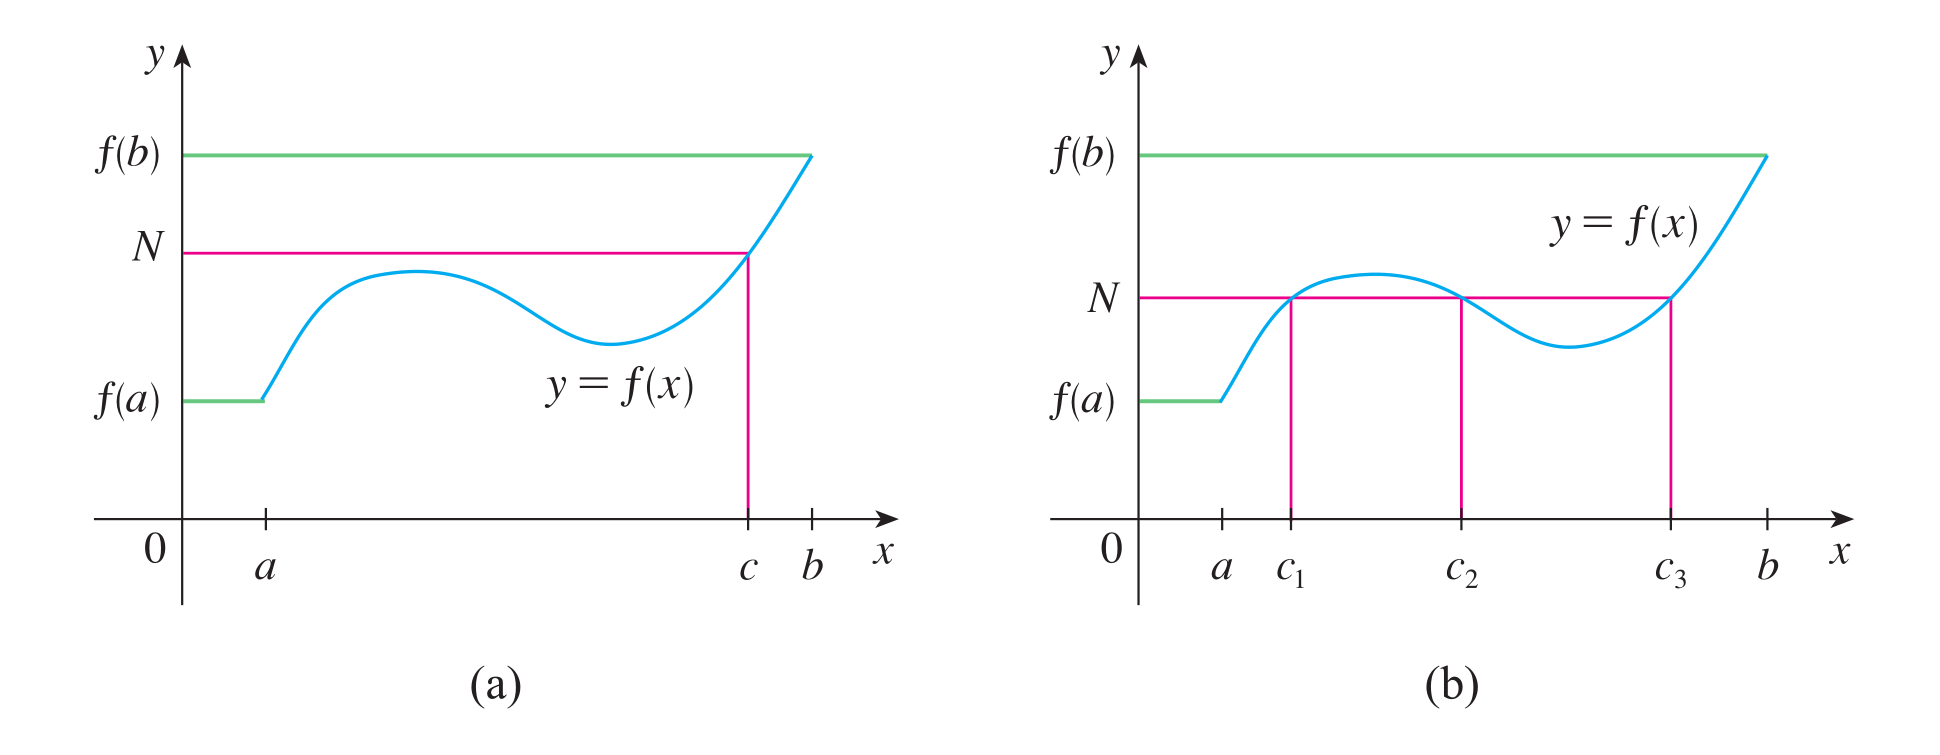
\includegraphics[width=0.9\linewidth]{res/in.png}
% 		\end{figure}
% 	\end{frame}
% 	\begin{frame}
% 		\frametitle{Types of Discontinuities}
% 		\begin{enumerate}
% 			\item removable discontinuity
% 			\item infinite discontinuity
% 			\item jump discontinuity
% 		\end{enumerate}
% 	\end{frame}
% 	\begin{frame}
% 		\frametitle{Exercise 1}
% 		Use the Intermediate Value Theorem to show that there is a root of the given equation in the specified interval.
% 		\begin{center}
% 			$\sqrt[3]{x} = 1 - x$,\ \ \ \ (0, 1)
% 		\end{center}
% 	\end{frame}
	
% 	\begin{frame}
% 		\frametitle{Exercise 1}
% 		Use the Intermediate Value Theorem to show that there is a root of the given equation in the specified interval.
% 		\begin{center}
% 			$\sqrt[3]{x} = 1 - x$,\ \ \ \ (0, 1)
% 		\end{center}
% 		Solution:
		
% 		$\sqrt[3]{x} = 1 - x$ has a root on (0, 1) equals to $f(x) = \sqrt[3]{x} + x -1 = 0$ has a solution on (0, 1).
		
% 		Since $f(0) = -1$, $f(1) = 1$, and 0 is between -1 and 1, there must be a point c such that $f(c) = 0$.
% 	\end{frame}

% 	\begin{frame}
% 		\frametitle{Exercise 2}
% 		Let $f(x) = \dfrac{e^{\frac{1}{x}} - 1}{e^{\frac{1}{x}} + 1}$. What kind of discontinuity is $x = 0$?
% 	\end{frame}
	
% 	\begin{frame}
% 		\frametitle{Exercise 2}
% 		Let $f(x) = \dfrac{e^{\frac{1}{x}} - 1}{e^{\frac{1}{x}} + 1}$. What kind of discontinuity is $x = 0$?
		
% 		Solution:
		
% 		$\lim\limits_{\textit{x} \to 0^-}f(x)=\dfrac{0-1}{0+1} = -1$
		
% 		$\lim\limits_{\textit{x} \to 0^+}f(x)=\dfrac{\infty - 1}{\infty + 1} = 1$
		
% 		Jump discontinuity.
% 	\end{frame}

% 	\begin{frame}
% 		\frametitle{Exercise 3}
% 		Find the values of $a$ and $b$ that make $f$ continuous everywhere.
% 		\begin{center}
% 			\begin{equation}
% 				f(x)=
% 				\begin{cases}
% 					\dfrac{x^{2} - 4}{x - 2} & x < 2\\
% 					ax^{2} - b{x} + 3 & 2 \leq x < 3\\
% 					2x - a - b & x \leq 3
% 				\end{cases}
% 			\end{equation}
% 		\end{center}
% 	\end{frame}
	
% 	\begin{frame}
% 		\frametitle{Exercise 3}
% 		Find the values of $a$ and $b$ that make $f$ continuous everywhere.
% 		\begin{center}
% 			\begin{equation}
% 				f(x)=
% 				\begin{cases}
% 					\dfrac{x^{2} - 4}{x - 2} & x < 2\\
% 					ax^{2} - b{x} + 3 & 2 \leq x < 3\\
% 					2x - a - b & x \leq 3
% 				\end{cases}
% 			\end{equation}
% 		\end{center}
		
% 		Solution:
		
% 		$\lim\limits_{\textit{x} \to 2^-}f(x)=\dfrac{(x-2)(x+2)}{(x-2)} = 4$
		
% 		$f(2)=4a-2b+3$
		
% 		$\lim\limits_{\textit{x} \to 3^-}f(x)=9a-3b+3$
		
% 		$f(3) = 6 - a -b$
		
% 		Let $\lim\limits_{\textit{x} \to 2^-}f(x)= f(2)$, $\lim\limits_{\textit{x} \to 3^-}f(x) = f(3)$ \rightarrow $a = \dfrac{1}{3}, b = \dfrac{1}{6}$
% 	\end{frame}

% 	\colortheme{blue!50!black}
% 	\begin{frame}
% 		\frametitle{Exercise 4}
% 		Find $a$ and $b$ that make $f(x) = \lim\limits_{\textit{n} \to +\infty}\dfrac{x^{2n - 1} + ax^{2} + bx}{x^{2n} + 1}$ continuous on ($-\infty$, $\infty$).
% 	\end{frame}
	
% 	\colortheme{blue!50!black}
% 	\begin{frame}
% 		\frametitle{Exercise 4}
% 		Find $a$ and $b$ that make $f(x) = \lim\limits_{\textit{n} \to +\infty}\dfrac{x^{2n - 1} + ax^{2} + bx}{x^{2n} + 1}$ continuous on ($-\infty$, $\infty$).
		
% 		Solution:
		
% 		$f(x) = \begin{cases}
% 					ax^2 + bx: -1<x<1\\
% 					\dfrac{a-b-1}{2}: x = -1\\
% 					\dfrac{a+b+1}{2}: x = 1\\
% 					\dfrac{1}{x}: x>1 \ or\  x<-1
% 				\end{cases}$
				
% 		At x = 1, 
% 		\begin{cases}
% 		$\dfrac{a+b+1}{2} = a+b$\\
% 		$a+b = 1$
% 		\end{cases}
		
% 		At x = -1,
% 		$a - b = -1$
		
% 		Thus, we have a = 0, b = 1
		
% 	\end{frame}

% 	\begin{frame}
% 		\frametitle{Exercise 5}
% 		There are two functions:\\
% 		$f(x)$ is continuous on ($-\infty$, $\infty$), and $f(x) \neq 0$.\\ 
% 		$\varphi (x)$ is defined on ($-\infty$, $\infty$), but $\varphi (x)$ has discontinuity.\\
% 		\bigskip
% 		Judge whether the following four statements are correct:
% 		\begin{enumerate}
% 			\item $\varphi [f(x)]$\ must have discountinuity.
% 			\item $[\varphi (x)]^{2}$\ must have discountinuity.
% 			\item Whether $f[\varphi (x)]$\ has discountinuity is uncertain.
% 			\item $\dfrac{\varphi (x)}{f(x)}$\ must have discountinuity.
% 		\end{enumerate}
% 	\end{frame}
	
% 	\begin{frame}
% 		\frametitle{Exercise 5}
% 		There are two functions:\\
% 		$f(x)$ is continuous on ($-\infty$, $\infty$), and $f(x) \neq 0$.\\ 
% 		$\varphi (x)$ is defined on ($-\infty$, $\infty$), but $\varphi (x)$ has discontinuity.\\
% 		\bigskip
% 		Judge whether the following four statements are correct:
% 		\begin{enumerate}
% 			\item $\varphi [f(x)]$\ must have discountinuity.
% 			\item $[\varphi (x)]^{2}$\ must have discountinuity.
% 			\item Whether $f[\varphi (x)]$\ has discountinuity is uncertain.
% 			\item $\dfrac{\varphi (x)}{f(x)}$\ must have discountinuity.
% 		\end{enumerate}
		
% 		Solution:
		
% \begin{enumerate}
%     \item No
%     \item No
%     \item Yes
%     \item Yes
% \end{enumerate}
% 	\end{frame}

% 	\colortheme{green!30!black}
% 	\begin{frame}{List of Limits}
% \begin{enumerate}[1]
%     \item $\lim\limits_{x \rightarrow a} c=c $
%     \item $\lim\limits_{x \rightarrow a} x^{n}=a^{n}$
%     \item $\lim\limits_{x \rightarrow 0} \dfrac{\sin x}{x}=1$
% \item $\lim\limits_{x \rightarrow 0} \dfrac{\tan x}{x}=1$
%     \item $\lim\limits_{x \rightarrow 0} \dfrac{1-\cos x}{x^{2}}=\dfrac{1}{2}$
%     \item $\lim\limits_{x \rightarrow 0} \dfrac{\arcsin x}{x}=1$
%     \item $\lim\limits_{x \rightarrow 0} \dfrac{e^{x}-1}{x}=1$
%     \item $\lim\limits_{x \rightarrow 0^{+}} x^{x}=1$
% \end{enumerate}
% \end{frame}
% \begin{frame}{List of Limits}
% \begin{enumerate}[1]
% \item $\lim\limits_{x \rightarrow 0^{+}} x \ln x=0$
%     \item $\lim\limits_{x \rightarrow 0} \dfrac{\sqrt[n]{x+1}-1}{x}=\dfrac{1}{n}$
%     \item $\lim\limits_{x \rightarrow \infty} x^{\frac{1}{x}}=1$
%     \item $\lim\limits_{x \rightarrow \pm \infty}\left(1+\dfrac{1}{x}\right)^{x}=e$
%     \item $\lim\limits_{x \rightarrow 0}(1+x)^{\frac{1}{x}}=e$
%     \item $\lim\limits_{x \rightarrow 0}(1+\sin x)^{\frac{1}{x}}=e$
%     \item $\lim\limits_{x \rightarrow \infty}\left(x-\sqrt{x^{2}-a^{2}}\right)=0$
% \item $\lim\limits_{x \rightarrow 0} \dfrac{\ln{(1+x)} }{x}=1$
% \end{enumerate}
% \end{frame}
	
% \begin{frame}
% 		\frametitle{References}
% 		[1] Huang, Yucheng. VV156\_RC2.pdf. 2021.\\
% 		\bigskip
% 		[2] Cai, Runze. Chapter01.pdf. 2021.\\
% 		\bigskip
% 		[3] Department of mathematics, Tongji University. Advanced Mathematics (7th Edition). 2014.\\
% 		\bigskip
% 		[4] James Stewart. Calculus (7th Edition). 2014.\\
% 		\bigskip
% 		[5] Department of mathematics, Tongji University. Learning Guidance of Advanced Mathematics (7th Edition). 2014.\\
% 		\bigskip
% 		[6]Zhou,Yishen.RC2. 2022.
% \end{frame}

% \section{Derivatives}
% \begin{frame}{Introduction}
%     \begin{block}{Tangent Line}
%         The \textbf{tangent line} to the curve $y=f(x)$ at the point $P(a, f(a))$ is the line through $P$ with slope
%         $$
%         m=\lim _{x \rightarrow a} \frac{f(x)-f(a)}{x-a}
%         $$
%         provided that this limit exists.
%     \end{block}
%     \begin{block}{Instantaneous rate of change}
%         $$
%         f^{\prime}(a)=\lim _{x \rightarrow a} \frac{f(x)-f(a)}{x-a}
%         $$$$
%         \text { instantaneous rate of change }=\lim _{\Delta x \rightarrow 0} \frac{\Delta y}{\Delta x}=\lim _{x_{2} \rightarrow x_{1}} \frac{f\left(x_{2}\right)-f\left(x_{1}\right)}{x_{2}-x_{1}}
%         $$
%     \end{block}
%     Try to define velocity in this way.
% \end{frame}

% \begin{frame}{Introduction}
%     $$
%         \text{average velocity} = \frac{\text{displacement}}{\text{time}} = \frac{f(a+h)-f(a)}{h}
%     $$
%     $$v(a)=\lim _{h\rightarrow 0}\frac{f(a+h)-f(a)}{h}$$
% \end{frame}

% \begin{frame}{Definition}
%     \begin{block}{Derivative}
%         The \textbf{derivative of a function \boldmath{$f$} at a number \boldmath{$a$}}, denoted by $f'(a)$, is
%         $$
%         f^{\prime}(a)=\lim _{x \rightarrow a} \frac{f(x)-f(a)}{x-a}
%         $$
%         if this limit exists.
%     \end{block}
%     The slope of the tangent line of a function is the corresponding derivative.
% \end{frame}

% \begin{frame}{Definition}
%     \begin{block}{Notations}
%         Newton: $$
%         \dot{y}
%         $$
%         Leibniz:
%         $$
%         \frac{d y}{d x}
%         $$
%         Lagrange:
%         $$
%         f^{\prime}(x)
%         $$
%         Jacobi: (Partial Derivatives)
%         $$
%         \frac{\partial f}{\partial x}
%         $$
%     \end{block}
% \end{frame}

% \begin{frame}{Differentiable}
%     \begin{block}{Differentiable}
%         A function $f$ is differentiable at $\boldsymbol{a}$ if $f^{\prime}(a)$ exists. It is differentiable on an open interval $(a, b)$ [or $(a, \infty)$ or $(-\infty, a)$ or $(-\infty, \infty)]$ if it is differentiable at every number in the interval.
%     \end{block}
%     \begin{block}{Differentiable and Continuity}
%         If $f$ is differentiable at $a$, then $f$ is continuous at $a$.
        
%         \textbf{NOTE} The converse of Theorem is false; that is, there are functions that are continuous but not differentiable. For instance, the function $f(x)=|x|$ is continuous at 0 because
%         $$
%         \lim _{x \rightarrow 0} f(x)=\lim _{x \rightarrow 0}|x|=0=f(0)
%         $$
%     \end{block}
% \end{frame}

% \begin{frame}{Differentiable}
%     The function is not differentiable at these points:
%     \bigskip
%     \begin{figure}[htbp]
%     \begin{center}
%     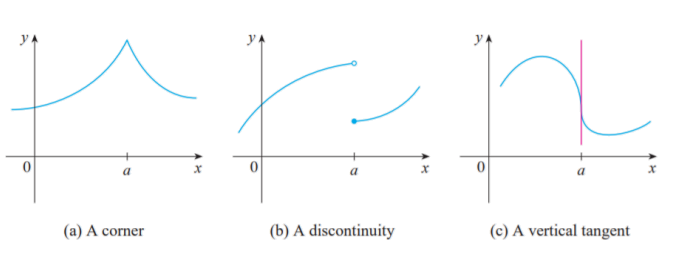
\includegraphics[width=1\textwidth]{res/4.png}
%     \end{center}
%     \end{figure}
% \end{frame}

% \begin{frame}{Higher derivatives}
%     $$
%     (f')' = f''\qquad \text{second derivative}
%     $$$$
%     (f'')' = f'''\qquad \text{third derivative}
%     $$
%     Example: still consider the position function
%     \begin{center}
%         position-velocity-acceleration-jerk-snap$\cdots$\\
%         $$
%         x-\frac{d y}{d t}-\frac{d^2 y}{d t^2}-\frac{d^3 y}{d t^3}-\frac{d^4 y}{d t^4}\cdots
%         $$
%     \end{center}
% \end{frame}

% \begin{frame}{Differential formulas}
%     $$
%     \frac{d}{d x}(C)=0 
%     $$$$
%     \frac{d}{d x}(x^{n})=n x^{n-1}
%     $$$$
%     (c f)^{\prime}=c f^{\prime}
%     $$$$
%     (f+g)^{\prime}=f^{\prime}+g^{\prime}
%     $$$$
%     (f-g)^{\prime}=f^{\prime}-g^{\prime}
%     $$$$
%     (f g)^{\prime}=f g^{\prime}+g f^{\prime}
%     $$$$
%     (\frac{f}{g})^{\prime}=\frac{g f^{\prime}-f g^{\prime}}{g^{2}}
%     $$
% \end{frame}

% \begin{frame}{Differential formulas}
%     $$
%     \begin{aligned}
%     &\frac{d}{d x}(\sin x)=\cos x \\
%     &\frac{d}{d x}(\csc x)=-\csc x \cot x \\
%     &\frac{d}{d x}(\cos x)=-\sin x \\
%     &\frac{d}{d x}(\sec x)=\sec x \tan x \\
%     &\frac{d}{d x}(\tan x)=\sec ^{2} x \\
%     &\frac{d}{d x}(\cot x)=-\csc ^{2} x
%     \end{aligned}
%     $$
% \end{frame}

% \begin{frame}{Differential formulas}
%     $$
%     \begin{aligned}
%     &\frac{d}{d x}\left(\sin ^{-1} x\right)=\frac{1}{\sqrt{1-x^{2}}} \\
%     &\frac{d}{d x}\left(\csc ^{-1} x\right)=-\frac{1}{x \sqrt{x^{2}-1}} \\
%     &\frac{d}{d x}\left(\cos ^{-1} x\right)=-\frac{1}{\sqrt{1-x^{2}}} \\
%     &\frac{d}{d x}\left(\sec ^{-1} x\right)=\frac{1}{x \sqrt{x^{2}-1}} \\
%     &\frac{d}{d x}\left(\tan ^{-1} x\right)=\frac{1}{1+x^{2}} \\
%     &\frac{d}{d x}\left(\cot ^{-1} x\right)=-\frac{1}{1+x^{2}}
%     \end{aligned}
%     $$
% \end{frame}

% \begin{frame}{Differential formulas}
%     $$
%     \begin{aligned}
%     &\frac{d}{d x}\left(\log _{a} x\right)=\frac{1}{x \ln a} \\
%     &\frac{d}{d x}(\ln x)=\frac{1}{x} \\
%     &\frac{d}{d x} \ln |x|=\frac{1}{x} \\
%     \end{aligned}
%     $$
% \end{frame}

% \begin{frame}
% 		\frametitle{Exercise 1}
% 		\framesubtitle{Images of a Function and Its Derivative}
% 			Find an equation of the tangent line to the curve $y = 2x\sin{x}$ at the point ($\dfrac{\pi}{2}$, $\pi$).
% 	\end{frame}
	
% \begin{frame}
% 		\frametitle{Exercise 1}
% 		\framesubtitle{Images of a Function and Its Derivative}
% 			Find an equation of the tangent line to the curve $y = 2x\sin{x}$ at the point ($\dfrac{\pi}{2}$, $\pi$).
			
% 			Solution: 
			
% 			$y' = 2(sinx + xcosx)$
			
% 			$k = y'(\dfrac{\pi}{2}) = 2$
			
% 			$y - \pi = 2(x - \dfrac{\pi}{2})$
			
% 			$ y - 2x = 0$
% 	\end{frame}


% \begin{frame}
% \frametitle{Exercise 2}
%     \framesubtitle{Basic Derivation Formula}
% 		Differentiate:
% 		\begin{enumerate}
% 			\item $y = x^{3} + \dfrac{7}{x^{4}} - \dfrac{2}{x} + 12$
% 			\item $y = \sin{x}\cos{x}$
% 			\item $y = \sqrt{x}\sin{x}$
% 			\item $y = 3e^{x}\cos{x}$
% 			\item $y = \dfrac{x\sin{x}}{1 + x}$
% 			\item $y = \dfrac{1 - \sec{x}}{\tan{x}}$
% 			\item $y = x^{2}\ln{x}\cos{x}$
% 			\item $y = \ln{3} + \dfrac{e^{x}}{x^{2}}$
% 		\end{enumerate}
% \end{frame}

% \begin{frame}{Exercise 2}
% Solution:

% \begin{enumerate}
%     \item $3x^2 - \dfrac{28}{x^5} + \dfrac{2}{x^2}$
%     \item cos2x
%     \item $\dfrac{1}{2}x^{-\frac{1}{2}}sinx + x^{\frac{1}{2}}cosx$
%     \item $3e^x(-sinx + cosx)$
%     \item $\dfrac{dy}{dx} = \dfrac{(xsinx)'(1+x)-xsinx}{(1+x)^2} = \dfrac{sinx + (1+x)xcosx}{(1+x)^2}$
%     \item $y = \dfrac{cosx-1}{sinx}  \rightarrow \dfrac{dy}{dx} = \dfrac{1}{1+cosx}$
%     \item $\dfrac{dy}{dx} = 2xlnxcosx + xcosx - x^2lnxsinx$
%     \item $(-2x^{-3} + x^{-2})e^x$
% \end{enumerate}
    
% \end{frame}

% \colortheme{blue!50!black}
% \begin{frame}
% 		\frametitle{Exercise 3}
% 		\framesubtitle{Basic Derivation Formula}
% 		Let $y = \log_{\varphi (x)}{f(x)}$\ ($\varphi (x) > 0$,\ $\varphi (x) \neq 1$,\ $f(x) > 0$). Suppose that both $\varphi (x)$ and $f(x)$ are differentiable. Calculate $\dfrac{dy}{dx}$.
% 	\end{frame}

% \begin{frame}{Exercise 3}
% Solution:

% $y = \dfrac{lnf(x)}{ln\varphi(x)}$

% $\dfrac{dy}{dx} = \dfrac{\frac{1}{f(x)}f'(x)ln\varphi(x) - \frac{1}{\varphi(x)}\varphi'(x)lnf(x)}{[ln\varphi(x)]^2}$

% $=\dfrac{f'(x)}{f(x)ln\varphi(x)} - \dfrac{\varphi'(x)lnf(x)}{\varphi(x)[ln\varphi(x)]^2}$

% \end{frame}

% \colortheme{green!30!black}

% \begin{frame}{Chain rule}
%     \begin{block}{Chain Rule}
%     If $g$ is differentiable at $x$ and $f$ is differentiable at $g(x)$, then the composite function $F=f \circ g$ defined by $F(x)=f(g(x))$ is differentiable at $x$ and $F^{\prime}$ is given by the product
%     $$
%     F^{\prime}(x)=f^{\prime}(g(x)) \cdot g^{\prime}(x)
%     $$
%     In Leibniz notation, if $y=f(u)$ and $u=g(x)$ are both differentiable functions, then
%     $$
%     \frac{d y}{d x}=\frac{d y}{d u} \frac{d u}{d x}
%     $$
%     \end{block}
% \end{frame}

% \begin{frame}{Chain rule}
%     \begin{block}{The Power Rule Combined with the Chain Rule }
%     If $n$ is any real number and $u=g(x)$ is differentiable, then
%     $$
%     \frac{d}{d x}\left(u^{n}\right)=n u^{n-1} \frac{d u}{d x}
%     $$
%     Alternatively,
%     $$
%     \frac{d}{d x}[g(x)]^{n}=n[g(x)]^{n-1} \cdot g^{\prime}(x)
%     $$
%     \end{block}
% \end{frame}
% \begin{frame}
% 		\frametitle{Exercise 4}
% 		\framesubtitle{Chain Rule}
% 		Find the derivative of the function:
% 		\begin{enumerate}
% 			\item $y = (4x - x^{2})^{100}$
% 			\item $y = 5^{-\frac{1}{x}}$
% 			\item $y = e^{-2x}\cos{4x}$
% 			\item $y = (\dfrac{x^{2}+1}{x^{2}-1})^{3}$
% 			\item $y = \dfrac{\arcsin{x}}{\arccos{x}}$
% 			\item $y = [\sin{(e^{(\sin{x})^{2}})}]^{2}$
% 			\item $y = \arcsin{\sqrt{\dfrac{1 - x}{1 + x}}}$
% 			\item $y = n^{n^{x}} + x^{n^{n}} + n^{x^{n}}$\ ($n > 0$,\ $n \neq 1$)
% 		\end{enumerate}
% 	\end{frame}
	
% \begin{frame}{Exercise 4}
%     \begin{enumerate}
%         \item $200(2-x)(4x-x^2)^{99}$
%         \item $ln5\cdot5^{-\frac{1}{x}}\cdot x^{-2}$
%         \item $-2e^{-2x}(cos4x + 2sin4x)$
%         \item $y' = 3(\dfrac{x^2+1}{x^2-1})^2(-\dfrac{2}{(x^2 - 1)^2})\cdot 2x = -\dfrac{12x(x^2+1)^2}{(x^2-1)^3}$
%         \item $y' = \dfrac{(arcsinx)'arccosx - (arccosx)'arcsinx}{(arccosx)^2} = \dfrac{arccosx + arcsinx}{\sqrt{1-x^2}(arccosx)^2}$
%         \item $y' = 2[sin(e^{(sinx)^2)}]\cdot cos(e^{(sinx)^2}) \cdot e^{(sinx)^2} \cdot 2sinxcosx = sin2x \cdot sin(2e^{(sinx)^2})\cdot e^{(sinx)^2}$
%         \item $y' = (1-\dfrac{1-x}{1+x})^{-\frac{1}{2}}\cdot \dfrac{1}{2}(\dfrac{1-x}{1+x})^{-\dfrac{1}{2}}[-\dfrac{2}{(x+1)^2}] = -\dfrac{1}{\sqrt{2x(1-x)}\cdot (x+1)}$
%         \item $y' = n^{n^x + x}(lnn)^2 + n^nx^{n^n -1} + n^{x^n + 1}x^{(n-1)}lnn$
%     \end{enumerate}
% \end{frame}

% \begin{frame}
% 		\frametitle{Exercise 5}
% 		\framesubtitle{Higher Derivative}
% 		Find the second derivative of the following function:\\
% 		(\alert{Warning}: Don't forget to double check your first derivative!)
% 		\begin{enumerate}
% 			\item $y = \tan{x}$
% 			\item $y = \dfrac{1}{x^{3} + 1}$
% 			\item $y = x\cos{x}$
% 		\end{enumerate}
% 	\end{frame}
	
% \begin{frame}{Exercise 5}
% \begin{enumerate}
%     \item $y' = sec^2x$
    
%     $y'' = 2secx \cdot (tanx \cdot secx) = 2tanx \cdot sec^2x$
%     \item $y' = -\dfrac{1}{(x^3 + 1)^2}\cdot 3x^2$
    
%     $y'' = -3 \cdot \dfrac{2x(x^3+1)^2 - 2(x^3+1)3x^4}{(x^3 + 1)^4} = \dfrac{6x(2x^3 - 1)}{(x^3 + 1)^3}$
%     \item $y' = cosx - xsinx$
    
%     $y'' = -2sinx - xcosx$
% \end{enumerate}
% \end{frame}

% \begin{frame}
% 		\frametitle{Exercise 6}
% 		\framesubtitle{Higher Derivative}
% 		 Answer the following three questions based on $\dfrac{dy}{dx} = y'$:
% 		\begin{enumerate}
% 			\item Express $\dfrac{dx}{dy}$ with $y'$
% 			\item Express $\dfrac{d^{2}x}{dy^{2}}$ with $y'$ and $y''$
% 			\item Express $\dfrac{d^{3}x}{dy^{3}}$ with $y'$ ,$y''$ and $y'''$
% 		\end{enumerate}
% 	\end{frame}
	
% \begin{frame}{Exercise 6}
% Solution:
% \begin{enumerate}
%     \item $\dfrac{dx}{dy} = \dfrac{1}{dy/dx} = \dfrac{1}{y'}$
%     \item $\dfrac{d^2x}{dy^2} = \dfrac{d}{dy}\cdot \dfrac{dx}{dy} = \dfrac{d}{dx}\dfrac{1}{y'}\dfrac{dx}{dy} = -\dfrac{y''}{(y')^3}$
%     \item $\dfrac{d^3x}{dy^3} = \dfrac{d}{dy}\dfrac{d^2x}{dy^2} = \dfrac{d}{dx}\dfrac{d^2x}{dy^2}\dfrac{dx}{dy} = - \dfrac{y'''(y')^3 - 3(y')^2(y'')^2}{(y')^6}\cdot \dfrac{1}{y'} = \dfrac{3y''' - y' (y'')^2}{(y')^5}$
% \end{enumerate}
    
% \end{frame}

% \begin{frame}{Implicit Differentiation}
%     \begin{block}{Find $y^{\prime}$ if $\sin (x+y)=y^{2} \cos x$}
%     Differentiating implicitly with respect to $x$ and remembering that $y$ is a function of $x$, we get
% $$
% \cos (x+y) \cdot\left(1+y^{\prime}\right)=y^{2}(-\sin x)+(\cos x)\left(2 y y^{\prime}\right)
% $$
% (Note that we have used the Chain Rule on the left side and the Product Rule and Chain Rule on the right side.) If we collect the terms that involve $y^{\prime}$, we get
% $$
% \cos (x+y)+y^{2} \sin x=(2 y \cos x) y^{\prime}-\cos (x+y) \cdot y^{\prime}
% $$
% So
% $$
% y^{\prime}=\frac{y^{2} \sin x+\cos (x+y)}{2 y \cos x-\cos (x+y)}
% $$
%     \end{block}
% \end{frame}
% \begin{frame}
% 		\frametitle{Exercise 7}
% 		\framesubtitle{Implicit Differentiation}
% 			Calculate the derivative of the following implicit function:
% 				\begin{enumerate}
% 					\item $y^{2} - 2xy + 9 = 0$
% 					\item $xy = e^{xy}$
% 				\end{enumerate}
% 	\end{frame}
% 	\begin{frame}{Solution}
% 	    \begin{enumerate}
% 	        \item $2yy'-2y-2xy'=0$,$y'=\dfrac{y}{y-x}$
% 	        \item The derivative does not exist!
% 	    \end{enumerate}
% 	\end{frame}
% \begin{frame}
% 		\frametitle{Exercise 8}
% 		\framesubtitle{Implicit Differentiation}
% 			Use \alert{logarithmatic differentiation} to calculate the derivative of the following implicit function:
% 				\begin{enumerate}
% 					\item $y = (\dfrac{x}{x + 1})^{x}$
% 					\item $y = \sqrt[5]{\dfrac{x - 5}{\sqrt[5]{x^{2} + 2}}}$
% 				\end{enumerate}
% 	\end{frame}
	
% \begin{frame}{Exercise 8}
%     Solution:
%     \begin{enumerate}
%         \item $lny = x[lnx - ln(x+1)]$
        
%         $\dfrac{1}{y}y' = [lnx - ln(x+1)] + x[\dfrac{1}{x} - \dfrac{1}{x+1}]$
        
%         $y' = (\dfrac{x}{x+1})^x [ln|\dfrac{x}{x+1}| + \dfrac{1}{x+1}]$
%         \item $lny = \dfrac{1}{5}ln|x-5| - \dfrac{1}{25}ln(x^2 + 2)$
        
%         $y'\dfrac{1}{y} = \dfrac{1}{5(x-5)} - \dfrac{2x}{25(x^2+2)}$
        
%         $y' = y[\dfrac{1}{5(x-5)} - \dfrac{2x}{25(x^2+2)}]$
%     \end{enumerate}
% \end{frame}


% \begin{frame}
% \frametitle{Exercise 9}
% \framesubtitle{Implicit Differentiation}
%     The \textit{Bessel function} of order $0, y=J(x)$, satisfies the differential equation $x y^{\prime \prime}+y^{\prime}+x y=0$ for all values of $x$ and its value at 0 is $J(0)=1$.\\
% (a) Find $J^{\prime}(0)$.\\
% (b) Use implicit differentiation to find $J^{\prime \prime}(0)$.
% \end{frame}

% \begin{frame}{Exercise 9}
% Solution:
% \begin{enumerate}
%     \item Take x=0, 0 + J'(0) + 0 = 0 $\rightarrow$ J'(0) = 0
%     \item xy''' + 2y'' + y + xy' = 0
    
%     At x = 0, 2y'' + 1 = 0, y'' = $-\dfrac{1}{2}$
% \end{enumerate}
    
% \end{frame}

% \begin{frame}{Linear approximation}
% \begin{block}{Definition}

% $$
% f(x) \approx f(a)+f^{\prime}(a)(x-a)
% $$
% is called the \textbf{linear approximation} or \textbf{tangent line approximation} of $f$ at $a$. The linear function whose graph is this tangent line, that is,\\

% $$
% L(x)=f(a)+f^{\prime}(a)(x-a)
% $$
% is called the linearization of $f$ at $a$.
% \end{block}
% \end{frame}
% \begin{frame}{Exercise 10}
%     \begin{block}{}
%     Use linear approximation to estimate $2.0006^{1.9998}$
%     \end{block}
% \end{frame}

% \begin{frame}{Exercise 10}
% Solution:
% $f(x) = 2^{x+2}$

% $f'(x) = 2^{x+2}ln2$

% $2^{1.9998} = f(0) + f'(0) \times (-0.0002) =  2^2 + 4ln2 \times (-0.0002) = 3.9994$

% $g(x) = (2+x)^{1.9998}$

% $g'(x) = 1.9998(2+x)^{0.9998}$

% $2.0006^{1.9998} = g(0) + g'(0)\times 0.0006 = 2^{1.9998} + 1.9998\times 2^{0.9998}\times 0.0006 = 4.0018$
    
% \end{frame}
% \begin{frame}{Equivalent Infinitesimal}
% \textbf{Tip:} You're highly recommended to remember this part!
%     $$
% \begin{aligned}
% &\textbf{When } x \rightarrow 0\\
% &a^{x}-1 \sim x \ln a \\
% &\arcsin (a) x \sim \sin (a) x \sim(a) x \\
% &\arctan (a) x \sim \tan (a) x \sim(a) x \\
% &\ln (1+x) \sim x \\
% &\sqrt{1+x}-\sqrt{1-x} \sim x \\
% &(1+a x)^{b}-1 \sim a b x \\
% &\sqrt[b]{1+a x}-1 \sim \frac{a}{b} x \\
% &1-\cos x \sim \frac{x^{2}}{2} \\
% &x-\ln (1+x) \sim \frac{x^{2}}{2} \\
% \end{aligned}
% $$
% \end{frame}


% \begin{frame}{Equivalent Infinitesimal}
%     $$
% \begin{aligned}
% &\textbf{When } x \rightarrow 0\\
% &\tan x-\sin x \sim \frac{x^{3}}{2}\\
% &\tan x-x \sim \frac{x^{3}}{3}\\
% &x-\arctan x \sim \frac{x^{3}}{3}\\
% &x-\sin x \sim \frac{x^{3}}{6}\\
% &\arcsin x-x \sim \frac{x^{3}}{6}\\
% \end{aligned}
% $$
% \end{frame}
% \begin{frame}{Equivalent Infinitesimal}
%     \begin{block}{Example: Solve the limit}
%     $$
%     \begin{aligned}
% \lim _{x \rightarrow 0} \frac{\ln (1+4 x)}{\sin (3 x)}&=\lim _{x \rightarrow 0} \frac{\ln (1+4 x)}{\sin (3 x)} \lim _{x \rightarrow 0} \frac{4 x}{\ln (1+4 x)} \lim _{x \rightarrow 0} \frac{\sin (3 x)}{3 x}\\&=\lim _{x \rightarrow 0} \frac{4 x}{3 x}=4 / 3
% \end{aligned}
% $$
%     \end{block}
%     For more exercise regarding to equivalent infinitesimal, please refer to Worksheet 1.
% \end{frame}
% \colortheme{blue!50!black}
% \begin{frame}{Taylor Expansion}
% \begin{block}{Definition}
%        Taylor expansion around x=x_0:\\
% $f(x)=f(x_0)+\sum\limits_{i=1}^n\frac{f^{(i)}(x)}{i!}(x-x_0)^i+R_n$, where $R_n=o[(x-x_0)^n]$\\
% \end{block}

% It simulates a function around a point with a polynomial function.
% \end{frame}
% \begin{frame}{Taylor Expansion}

% Taylor expansion of some polynomials when x is around 0:
% \begin{enumerate}
%     \item $e^x=1+x+\frac{x^2}{2}+\frac{x^3}{6}+o(x^3)$
%     \item $ln(1+x)=x-\frac{x^2}{2}+\frac{x^3}{3}+o(x^3)$
%     \item $sinx=x-\frac{x^3}{6}+\frac{x^5}{120}+o(x^5)$
%     \item $cosx=1-\frac{x^2}{2}+\frac{x^4}{24}+o(x^4)$
%     \item $tanx=x+\frac{x^3}{3}+\frac{2x^5}{15}+o(x^5)$
% \end{enumerate}
% \begin{block}{Tip}
% \footnotesize
% o(x^n)\ means\ the\ order\ of\ the\ polynomial\ is\ \alert{larger}\ than\ n;\\
% O(x^n)\ means\ the\ order\ of\ the\ polynomial\ is\ \alert{larger\ than\ or\ equal\ to}\ n.
% \normalsize
% \end{block}
% \end{frame}
% \begin{frame}{Taylor Expansion}
    

% The transformation of Taylor Expansion:
% \begin{block}{Example}
% The Taylor expansion of $e^{x^2}$ around\ x=0:\\
% $e^{x^2}=1+x^2+\frac{(x^2)^2}{2}+\frac{(x^2)^3}{6}+o((x^2)^3)=1+x^2+\frac{x^4}{2}+\frac{x^6}{6}+o(x^6)$
% \end{block}


% \end{frame}
% \begin{frame}{Exercise 11}
% \begin{block}{}
% \begin{enumerate}
%     \item Calculate The Taylor expansion of:\\
% \begin{enumerate}
%     \item $e^{sinx}$ around\ x=0 (below degree 4)
%     \item $ln(2+x)$ around\ x=-1 (below degree 4)
% \end{enumerate}
% \item Calculate the limit $$\lim\limits_{x\to 0}\frac{ln(e^{sinx}+sinx)-ln(e^{tanx}+tanx)}{x^2\cdot tanx}$$
% \end{enumerate}

% \end{block}
    
% \end{frame}
% \begin{frame}{Exercise 11}
% \small
%     Solution:\\
%     (1)\\
%     \begin{enumerate}
%         \item $e^{sinx}=1+(x-\dfrac{1}{6}x^3+O(x^5))+\dfrac{1}{2}(x-\dfrac{1}{6}x^3+O(x^5))^2+\dfrac{1}{6}(x+O(x^3))^3+\dfrac{1}{24}(x+O(x^3))^4=1+x+\dfrac{x^2}{2}-\dfrac{x^4}{8}+O(x^5)$
%         \item $ln(2+x)=ln(1+(1+x))=ln(1+x)=(1+x)-\frac{(1+x)^2}{2}+\frac{(1+x)^3}{3}-\frac{(1+x)^4}{4}+O((1+x)^5)$
%     \end{enumerate}
% \end{frame}
% \begin{frame}{Exercise 11}
%     Solution:\\
%     (2)\\
%     The denominator's Taylor expansion is $x^2tanx=x^3+O(x^5)$, thus for the numerator we can ignore elements of degree 4 or higher.\\
%     \begin{enumerate}
%         \item $e^x+x=1+2x+\dfrac{x^2}{2}+\dfrac{x^3}{6}+O(x^4)$
%         \item $ln(e^x+x)=2x+\dfrac{x^2}{2}+\dfrac{x^3}{6}-\dfrac{1}{2}(2x+\dfrac{x^2}{2}+\dfrac{x^3}{6})^2+\dfrac{1}{3}(2x+\dfrac{x^2}{2}+\dfrac{x^3}{6})^3+O(x^4)=2x-\dfrac{3}{2}x^2-\dfrac{1}{2}x^3+O(x^4)$
%         \item $ln(e^{sinx}+sinx)=2x-\dfrac{1}{3}x^3-\dfrac{3}{2}x^2-\dfrac{1}{2}x^3+O(x^4)$
%         \item$ln(e^{tanx}+tanx)=2x+\dfrac{2}{3}x^3-\dfrac{3}{2}x^2-\dfrac{1}{2}x^3+O(x^4)$
%     \end{enumerate}
%     \begin{center}
%         $ans=\dfrac{-x^3}{x^3}=-1$
%     \end{center}
% \normalsize
    
% \end{frame}
% \colortheme{green!30!black}
% \begin{frame}{Maximum and minimum}
%      \begin{block}{Absolute Maximum and Absolute Minimum}
% Let $c$ be a number in the domain $D$ of a function $f$. Then $f(c)$ is the 

% - \textbf{absolute maximum} value of $f$ on $D$ if $f(c) \geqslant f(x)$ for all $x$ in $D$. 

% - \textbf{absolute minimum} value of $f$ on $D$ if $f(c) \leqslant f(x)$ for all $x$ in $D$.
%     \end{block}
%     \begin{block}{Local Maximum and Local Minimum}
% The number $f(c)$ is a

% - \textbf{local maximum} value of $f$ if $f(c) \geqslant f(x)$ when $x$ is near $c$.

% - \textbf{local minimum} value of $f$ if $f(c) \leqslant f(x)$ when $x$ is near $c$.
%     \end{block}
%     \begin{block}{Critical number}
%         A \textbf{critical number} of a function $f$ is a number $c$ in the domain such that either $f^\prime (c)=0$ or $f^\prime (c)$ does not exist.
%     \end{block}
%     local maximum/minimum $\rightarrow$ critical number
% \end{frame}

% \begin{frame}{Related Theorems}
%     \begin{block}{The Extreme Value Theorem}
% If $f$ is continuous on a closed interval $[a, b]$, then $f$ attains an absolute maximum value $f(c)$ and an absolute minimum value $f(d)$ at some numbers $c$ and $d$ in $[a, b]$.
%     \end{block}
%     \begin{block}{Fermat's Theorem}
% If $f$ has a local maximum or minimum at $c$, and if $f^{\prime}(c)$ exists, then $f^{\prime}(c)=0$.
%     \end{block}
%     \begin{block}{Rolle's Theorem}
%  Let $f$ be a function that satisfies the following three hypotheses:
 
% 1. $f$ is continuous on the closed interval $[a, b]$.

% 2. $f$ is differentiable on the open interval $(a, b)$.

% 3. $f(a)=f(b)$

% Then there is a number $c$ in $(a, b)$ such that $f^{\prime}(c)=0$.
%     \end{block}
% \end{frame}
% \begin{frame}{Related Theorems}
%     \begin{block}{Lagrange Mean Value Theorem }
% Let $f$ be a function that satisfies the following hypotheses:

% 1. $f$ is continuous on the closed interval $[a, b]$.

% 2. $f$ is differentiable on the open interval $(a, b)$.

% Then there is a number $c$ in $(a, b)$ such that
% $$
% f^{\prime}(c)=\frac{f(b)-f(a)}{b-a}
% $$
% or, equivalently,
% $f(b)-f(a)=f^{\prime}(c)(b-a)$
%     \end{block}
% \end{frame}
% \begin{frame}{Related Theorems}
%     \begin{block}{Cauchy Mean Value Theorem (Extended Mean Value Theorem) }
% Let $f,g$ be two functions that satisfy the following hypotheses:

% 1. $f,g$ is continuous on the closed interval $[a, b]$.

% 2. $f,g$ is differentiable on the open interval $(a, b)$.

% 3.$x \in(a, b), g^{\prime}(x) \neq 0$

% Then there is a number $c$ in $(a, b)$ such that
% $$
% \frac{f(b)-f(a)}{g(b)-g(a)}=\frac{f^{\prime}(c)}{g^{\prime}(c)}
% $$
% or, equivalently,
% $(f(b)-f(a)) g^{\prime}(c)=(g(b)-g(a)) f^{\prime}(c)$
%     \end{block}
% \end{frame}

% \begin{frame}
% \frametitle{Exercise 12}
% \framesubtitle{The Mean Value Theorem}
%     Verify that the function satisfies the hypotheses of the Mean Value Theorem on the given interval. Then find all numbers $c$ that satisfy the conclusion of the Mean Value Theorem.
% \begin{enumerate}
% \item $f(x)=x^{3}-3 x+2, \quad[-2,2]$
% \item $f(x)=\ln x, \quad[1,4]$
% \end{enumerate}
% \end{frame}

% \begin{frame}{Exercise 12}
% Solutions:
% \begin{enumerate}
%     \item f(-2) = 0, f(2) = 4
    
%     $k = \dfrac{f(2) - f(-2)}{4} = 1$
    
%     $f'(x) = 3x^2 - 3, 3c^2 - 3 = 1$
    
%     $c = \dfrac{2\sqrt{3}}{3}$
%     \item 
%     $k = \dfrac{f(4) - f(1)}{3} = \dfrac{2ln2}{3}$
    
%     $f'(x) = \dfrac{1}{x}$
    
%     $d = \dfrac{3}{2ln2}$
    
% \end{enumerate}
% \end{frame}



% \begin{frame}{Relationship between $f^\prime$ and $f$}
%     \begin{block}{Increasing/Decreasing Test}
%         If $f^\prime(x)>0$ on an interval, then $f$ is increasing on that interval.\\
%         If $f^\prime(x)<0$ on an interval, then $f$ is decreasing on that interval.\\
%     \end{block}
%     \begin{block}{The First Derivative Test}
%         Suppose that $c$ is a critical number of a continuous function $f$.\\
%         If $f^\prime$ changes from positive to negative at $c$, $f$ has a local maximum at $c$.\\
%         If $f^\prime$ changes from negative to positive at $c$, $f$ has a local minimum at $c$.\\
%         If $f^\prime$ does not change sign at $c$, $f$ has no local maximum or minimum at $c$.
%     \end{block}
% \end{frame}

% \begin{frame}{Relationship between $f^{\prime\prime}$ and $f$}
%     \begin{block}{Concave upward/downward}
%         If the graph of $f$ lies above all of its tangents on an interval $I$, then it is called \textbf{concave upward} on $I$. If the graph of $f$ lies below all of its tangents on an interval $I$, then it is called \textbf{concave downward} on $I$.
%     \end{block}
%     \begin{block}{Concavity Test}
%         If $f^{\prime\prime}(x)>0$ for all $x$ in $I$, then the graph of $I$ is concave upward on $I$.\\
%         If $f^{\prime\prime}(x)<0$ for all $x$ in $I$, then the graph of $I$ is concave downward on $I$.
%     \end{block}
% \end{frame}

% \begin{frame}{Relationship between $f^{\prime\prime}$ and $f$}
%     \begin{block}{Inflection point}
%         A point $P$ on a curve $y=f(x)$ is called an \textbf{inflection point} if $f$ is continuous there and the curve changes from concave upward to concave downward or from concave downward to concave upward at $P$.
%     \end{block}
%     \begin{block}{The Second Derivative Test}
%         Suppose $f^{\prime\prime}$ is continuous near $c$.\\
%         If $f^\prime(c)=0$ and $f^{\prime\prime}(c)>0$, then $f$ has a local minimum at $c$.\\
%         If $f^\prime(c)=0$ and $f^{\prime\prime}(c)<0$, then $f$ has a local maximum at $c$.
%     \end{block}
% \end{frame}
% \begin{frame}{L'Hospital's Rule}
%     \begin{block}{L'Hospital's Rule}
%         Suppose $f$ and $g$ are differentiable and $g^\prime(x)\neq0$ on an open interval $I$ that contains $a$ (except possibly at $a$). Suppose that\\
%         $$
%         \lim_{x\rightarrow a}f(x)=0\quad \text{and}\quad \lim_{x\rightarrow a}g(x)=0
%         $$
%         or that
%         $$
%         \lim_{x\rightarrow a}f(x)=\pm\infty\quad \text{and}\quad \lim_{x\rightarrow a}g(x)=\pm\infty
%         $$
%         (In other words, we have an indeterminate form of type $\frac{0}{0}$ or $\infty/\infty$.) Then\\
%         $$
%         \lim_{x\rightarrow a}\frac{f(x)}{g(x)}=\lim_{x\rightarrow a}\frac{f^\prime(x)}{g^\prime(x)}
%         $$
%         if the limit on the right side exists (or is $\infty$ or $-\infty$).
%     \end{block}
% \end{frame}




% \begin{frame}
% 		\frametitle{Exercise 13}
% 		\framesubtitle{l'Hôpital's rule}
% 		\alert{Warning}: Always judge whether l'Hôpital's rule can be applied before you use it, and \alert{don't neglect those basic methods of finding the limit}.\\
% 		\bigskip
% 		Evaluate the following limits:
% 		\begin{enumerate}
% 			\item $\lim\limits_{\textit{x} \to 0^{+}}x^{\sin{x}}$
% 			\item $\lim\limits_{\textit{x} \to 1}\dfrac{\ln x}{x-1}$
% 			\item $\lim\limits_{\textit{x} \to \infty}x^{3}e^{-x^{2}}$
% 			\item $\lim\limits_{\textit{x} \to \infty}[x - x^{2}\ln{\dfrac{x + 1}{x}}]$\\
% 				\begin{figure}
% 					
\includegraphics[width=0.1\linewidth]{res/troll.png}
% 				\end{figure}
% 			\item \begin{center}
% 					$\lim\limits_{\textit{x} \to \infty}\dfrac{x}{\sqrt{x^{2} + 1}}$
% 				\end{center}
% 		\end{enumerate}
% 	\end{frame}

% \begin{frame}{Exercise 13}
% Solution:
% \begin{enumerate}
%     \item 1
%     \item 1
%     \item $\lim\limits_{\textit{x} \to \infty}\dfrac{x^3}{e^{x^2}} = \lim\limits_{\textit{x} \to \infty} \dfrac{3x^2}{2xe^{x^2}} = \lim\limits_{\textit{x} \to \infty} \dfrac{6x}{(2 + 4x^2)e^{x^2}} =  \lim\limits_{\textit{x} \to \infty} \dfrac{6}{12x + 8x^2} = 0$
%     \item $ u = \dfrac{1}{x}$
    
    
%     $\lim\limits_{\textit{u} \to 0} \dfrac{u - ln(u+1)}{u^2} = \lim\limits_{\textit{u} \to 0} \dfrac{1 - \dfrac{1}{u+1}}{2u} = \lim\limits_{\textit{u} \to 0} \dfrac{\dfrac{1}{(u+1)^2}}{2} = \dfrac{1}{2}$
%     \item $\lim\limits_{\textit{x} \to \infty} \dfrac{\sqrt{x^2 + 1}}{x} = 1$
% \end{enumerate}
    
% \end{frame}


% \begin{frame}{References}
	
% 	[1] Huang, Yucheng. VV156\_RC2.pdf. 2021.\\
% 	\bigskip
% 	[2] Huang, Yucheng. VV156\_RC3.pdf. 2021.\\
% 	\bigskip
% 	[3] Cai, Runze. Chapter02.pdf. 2021.\\
% 	\bigskip
% 	[4] Cai, Runze. Chapter03.pdf. 2021.\\
% \bigskip
% 	[5] Department of mathematics, Tongji University. Advanced Mathematics (7th Edition). 2014.\\
% 		\bigskip
% 		[6] James Stewart. Calculus (7th Edition). 2014.\\
% 		\bigskip
% 		[7] Department of mathematics, Tongji University. Learning Guidance of Advanced Mathematics (7th Edition). 2014.\\
% 		\bigskip
% 		[8]Huang, Jiahe, Zhou Yishen. VV156 RC3. 2022\\
% \end{frame}


% \section{Integral}
% \begin{frame}{Antiderivatives}
% \begin{block}{Definition}
%     A function \textit{F} is called an antiderivative of \textit{f} on an interval \textit{I} if \textit{F′(x) = f(x)} for all \textit{x} in \textit{I}.
% \end{block}
% \begin{block}{Theorem}
%     If \textit{F} is an antiderivative of \textit{f} on an interval \textit{I}, then the most general antiderivative of \textit{f} on \textit{I} is $$F(x)+C$$,
%     where C is an arbitrary constant.
% \end{block}
% \begin{center}
%     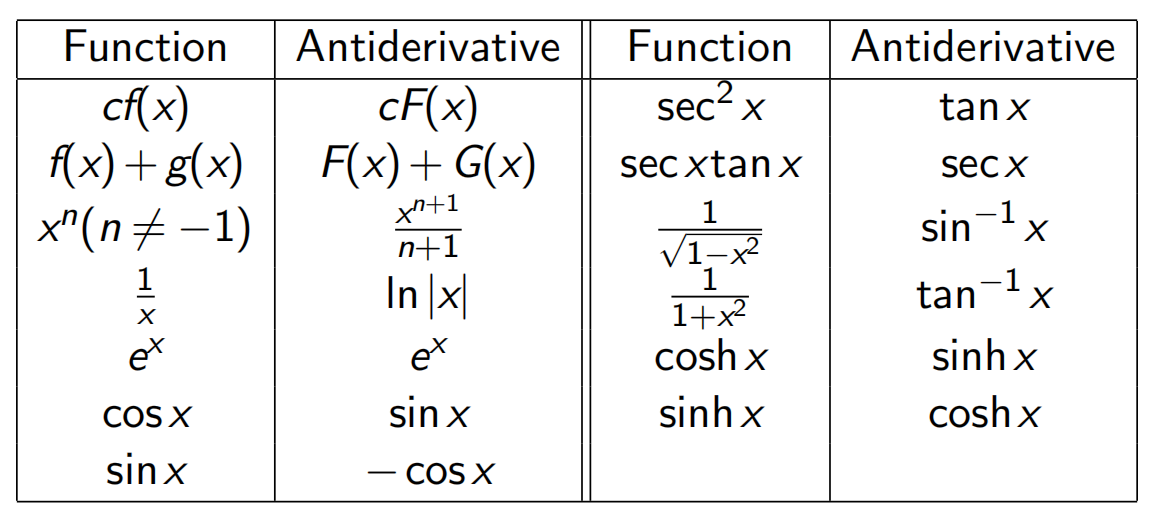
\includegraphics[height=3cm]{res/anti.png}
% \end{center}

% \end{frame}

% \begin{frame}{Antiderivatives}
% \begin{block}{notation}
%     $$
% \int f(x) d x=F(x) \quad \text { means } \quad F^{\prime}(x)=f(x)
% $$
% \end{block}
% How to understand this notation?
%     \begin{block}{Theorem}
%         If the antiderivatives of functions \textit{f(x)} and \textit{g(x)} exist, then for any constant \textit{p} and \textit{q}, the antiderivate of \textit{pf(x)+qg(x)} also exists, and we have
%         $$\int[pf(x)+qg(x)]dx=p\int f(x)dx+q\int g(x)dx$$
%     \end{block}
% \end{frame}

% \begin{frame}{Indefinite Integrals}
% Keep the following indefinite integrals firmly in mind!\\
% $$
% \begin{array}{ll}
% \int c f(x) d x=c \int f(x) d x & \int[f(x)+g(x)] d x=\int f(x) d x+\int g(x) d x \\
% \int k d x=k x+C & \int \dfrac{1}{x} d x=\ln \alert{|}x\alert{|}+C \\
% \int x^{n} d x=\dfrac{x^{n+1}}{n+1}+C & \int a^{x} d x=\dfrac{a^{x}}{\ln a}+C \\
% \int e^{x} d x=e^{x}+C & \int \cos x d x=\sin x+C \\
% \int \sin x d x=-\cos x+C & \int \csc ^{2} x d x=-\cot x+C \\
% \int \sec ^{2} x d x=\tan x+C & \int \csc x \cot x d x=-\csc x+C \\
% \int \sec x \tan x d x=\sec x+C & \int \dfrac{1}{\sqrt{1-x^{2}}} d x=\arcsin x+C \\
% \int \dfrac{1}{x^{2}+1} d x=\arctan x+C & \int \cosh x d x=\sinh x+C \\
% \int \sinh x d x=\cosh x+C 
% \end{array}
% $$
% \end{frame}

% \begin{frame}{Substitution Rule}
%     \begin{block}{Definition}
%     $$
% \int f(x) g^{\prime}(x) dx= \int f(x)dg(x)
% $$
%     \end{block}
%     How to memorize?\\
%     $\dfrac{dg(x)}{dx}=g^{\prime}(x)$\\$\Rightarrow dx=\dfrac{dg(x)}{g^{\prime}(x)}$\\$\Rightarrow \int f(x) g^{\prime}(x) dx= \int f(x)g^{\prime}(x)\cdot \dfrac{dg(x)}{g^{\prime}(x)}=\int f(x)dg(x)$
% \end{frame}

% \begin{frame}{Substitution Rule}
% Type 1: Direct Substitution ($u=g(x)$)
% \begin{block}{Substitution Rule for Direct Substitution}
% If $u=g(x)$ is a differentiable function whose range is an interval $I$ and $f$ is continuous on $I$, then
% $$
% \int f(g(x)) g^{\prime}(x) dx= \int f(g(x))dg(x)=\int f(u) d u=F(u)+C
% $$
% \end{block}
% Type 2: Inverse Substitution ($x=\varphi(t)$)
% \begin{block}{Substitution Rule for Inverse Substitution}
% If $x=\varphi(t)$ is an invertible function, then
% $$
% \int f(x)dx = \int f(\varphi (t))d\varphi (t)=\int f(\varphi (t))\varphi ^{\prime}(t)dt=\widetilde{F}(t)=\widetilde{F}(\varphi ^{-1}(x))+C
% $$
% \end{block}
% \end{frame}

% \begin{frame}{Exercise 1}
%     \begin{enumerate}
%         \item$\int\dfrac{3x^3}{1-x^4}dx$
%         \bigskip
%         \item $\int\dfrac{ln x}{x}dx$
%         \bigskip
%         \item $\int\dfrac{sec^2 x}{tan^{10} x}dx$
%     \end{enumerate}
% \end{frame}

% \colortheme{blue!50!black}

% \begin{frame}{Substitution Rule}
% An Important Application: Trigonometric Substitutions:
% $$
% \begin{aligned}
% &\begin{array}{|c|c|c|}
% \hline \text { Expression } & \text { Substitution } & \text { Identity } \\
% \hline \sqrt{a^{2}-x^{2}} & x=a \sin \theta, \quad-\frac{\pi}{2} \leqslant \theta \leqslant \frac{\pi}{2} & 1-\sin ^{2} \theta=\cos ^{2} \theta \\
% \sqrt{a^{2}+x^{2}} & x=a \tan \theta, \quad-\frac{\pi}{2}<\theta<\frac{\pi}{2} & 1+\tan ^{2} \theta=\sec ^{2} \theta \\
% \sqrt{x^{2}-a^{2}} & x=a \sec \theta, \quad 0 \leqslant \theta<\frac{\pi}{2} & \sec ^{2} \theta-1=\tan ^{2} \theta \\
% \hline
% \end{array}
% \end{aligned}
% $$
% \end{frame}


% \begin{frame}{Exercise 2}
%     $\int\dfrac{1}{x^2\sqrt{x^2+4}}$
% \end{frame}
% \colortheme{green!30!black}
% \begin{frame}{Integration by Parts}
% $$
% \int u d v=u v-\int v d u
% $$
% $$
% \int f(x) g^{\prime}(x) d x=f(x) g(x)-\int g(x) f^{\prime}(x) d x
% $$
% How to choose $f(x)$ and $g'(x)$?\\
% \bigskip
% Among the following function types:\\
% the more to the left, the more suitable to be $f(x)$\\
% the more to the right, the more suitable to be $g'(x)$\\
% \bigskip
% \alert{(left)} inverse trigonometric function, logarithm function, power function, trigonometric function, exponential function \alert{(right)}
% \end{frame}
% \begin{frame}{Applicable Situations}
% When should we consider applying Integration by Parts?
% \begin{enumerate}
% \item If the integrand is the product of \alert{inverse trigonometric function, logarithm function or power function} and another function \alert{whose antiderivative is easy to calculate}.
% \item If the integrand is the product of \alert{trignometric function and exponential function}, apply Integration by Part twice in order to find an identical equation about the original integral, and then solve that equation.
% \item If the integrand contains $n$ (or a relatively large number), apply Integration by Part to \alert{find the recursion formula}. 
% \end{enumerate}
% \end{frame}

% \begin{frame}{Exercise 3}
%     \begin{enumerate}
%         \item $\int xsinx\ dx$
%         \bigskip
%         \item $\int ln^2x\ dx$
%         \bigskip
%         \item $\int x^2e^x\ dx$
%     \end{enumerate}
% \end{frame}

% \colortheme{blue!50!black}

% \begin{frame}{$\int sin^mx\ cos^nx\ dx$}
% \begin{enumerate}
%     \item If at least m and n is odd, adopt substitution rule.
%     \bigskip
%     $\int sin^mxcos^{2n+1}xdx=\int sin^mxcos^{2n}xd(sinx)=\int sin^mx\cdot(1-sin^2x)^nd(sinx)\overset{\text{u=sinx}}{=}\int u^m(1-u^2)^ndu$\\
%     \bigskip
%     $\int cos^mxsin^{2n+1}xdx=-\int cos^mxsin^{2n}xd(cosx)=-\int cos^mx\cdot(1-cos^2x)^nd(cosx)\overset{\text{u=cosx}}{=}-\int u^m(1-u^2)^ndu$\\
%     \bigskip
%     \item Else, use half-angle identities that $sin^2x=\dfrac{1}{2}(1-cos2x)$, $cos^2x=\dfrac{1}{2}(1+cos2x)$.
    
% \end{enumerate}
% \end{frame}

% \begin{frame}{$\int sec^mx\ tan^nx\ dx$}
%     \begin{enumerate}
%         \item If m is even (not 0), use $d(tanx)=sec^2xdx$ to transform it into the integration of tanx.\\
%         \bigskip
%         $\int sec^{2k}xtan^nxdx=\int (tan^2x+1)^ktan^nxd(tanx)\overset{\text{u=tanx}}{=}\int (u^2+1)^ku^ndu$.
%         \item If n is odd, use$d(secx)=secxtanxdx$ to transform it into the integration of secx.\\
%         \bigskip
%         $\int tan^{2k+1}xsec^ndx=\int (sec^2x-1)^ksec^{n-1}d(secx)=\cdots$
%     \end{enumerate}
%     Though not as useful, you can also explore $\int csc^mxcot^nxdx$.
% \end{frame}

% \begin{frame}{$\int sin mx\ cos nx\ dx$}
%     Use Product-to-Sum formula:
%     \begin{enumerate}
%         \item $sin\alpha cos\beta=\dfrac{1}{2}(sin(\alpha+\beta)+sin(\alpha-\beta))$
%         \item $cos\alpha sin\beta=\dfrac{1}{2}(sin(\alpha+\beta)-sin(\alpha-\beta))$
%         \item $sin\alpha sin\beta=\dfrac{1}{2}(cos(\alpha+\beta)+cos(\alpha-\beta))$
%         \item $cos\alpha cos\beta=-\dfrac{1}{2}(cos(\alpha+\beta)-cos(\alpha-\beta))$
%     \end{enumerate}
% \end{frame}



% \begin{frame}{Exercise 4}
%     \begin{enumerate}
%         \item $\int\limits_0^{\pi/2} sin^7xcos^5x\ dx$
%     \end{enumerate}
% \end{frame}

% \begin{frame}{Exercise 1-4 Answer}
% \scriptsize
%     Exercise 1:
%     \begin{enumerate}
%         \item ans=$0.75\int\dfrac{1}{1-x^4}dx^4$=$-\dfrac{3}{3}\int\dfrac{1}{1-x^4}d(1-x^4)$=$-\dfrac{3}{4}ln|1-x^4|+C$
%         \item $d(ln x)=dx\cdot \dfrac{1}{x} \Rightarrow ans= \int lnx d(lnx)=\dfrac{1}{2}ln^2x+C$
%         \item $d(tanx)=sec^2x\cdot dx\Rightarrow ans=\int \dfrac{d (tanx)}{tan^{10} x}=-\dfrac{1}{9}tan^{-9}x+C$
%     \end{enumerate}
%     Exercise 2:\\
%     Let $x=:2tan\theta$, $\theta\in(-\dfrac{\pi}{2},\dfrac{\pi}{2})$, $\dfrac{dx}{d\theta}=2sec^2\theta$,$\sqrt{x^2+4}=2sec\theta$, ans=$\int \dfrac{cos\theta}{4sin^2\theta}d\theta$.\\
%     Then $u:=sin\theta$, ans=$\int\dfrac{du}{4u^2}$=$-\dfrac{1}{4u}+C$=$-\dfrac{1}{4sin\theta}$+C=$\dfrac{-\sqrt{x^2+4}}{4x}+C$\\
%     Exercise 3:
%     \begin{enumerate}
%         \item ans=$-\int xd(cosx)$=$-xcosx+\int cosx dx$=$-xcosx+sinx+C$
%         \item ans=$xln^2x-\int 2lnxdx=xln^2x-2xlnx+\int 2dx=xln^2x-2xlnx+2x+C$
%         \item ans=$x^2e^x-2\int xe^xdx$=$x^2e^x-2xe^x+2\int e^xdx=(x^2-2x+2)e^x+C$
%     \end{enumerate}
%     Exercise 4:
%     \begin{enumerate}
%         \item $\int\limits_0^{\pi/2} sin^7xcos^5x\ dx=\int\limits_0^{1} sin^7x(1-sin^2x)^2 d(sinx)=[\dfrac{1}{8}u^8-\dfrac{1}{5}u^{10}+\dfrac{1}{12}u^{12}]_{0}^{1}=\dfrac{1}{120}$
%     \end{enumerate}
    
% \normalsize
% \end{frame}

% \begin{frame}{$\int e^{ax}sin^nx\ dx$}
%     \small
%     Use \textbf{induction}.\\
%     \bigskip
%     $\int e^{ax}sin^nx\ dx$\\
%     $=\dfrac{1}{a}\int sin^nx\ d(e^{ax})$\\
%     $=\dfrac{1}{a}e^{ax}sin^nx-\dfrac{n}{a}\int e^{ax}sin^{n-1}xcosx\ dx$\\
%     $= \dfrac{1}{a}e^{ax}sin^nx-\dfrac{n}{a^2} e^{ax}sin^{n-1}xcosx+\dfrac{n}{a^2}\int e^{ax}((n-1)sin^{n-2}cos^2x-sin^nx)\ dx$\\ $=\dfrac{1}{a}e^{ax}sin^nx-\dfrac{n}{a^2} e^{ax}sin^{n-1}xcosx+\dfrac{n}{a^2}\int e^{ax}((n-1)sin^{n-2}-nsin^nx)\ dx$\\
%     \bigskip
%     $\Rightarrow$\\
%     \bigskip
%     $\dfrac{a^2+n^2}{a^2}\int e^{ax}sin^nx\ dx=\dfrac{e^{ax}sin^{n-1}x}{a}(sinx-\dfrac{n}{a} cosx)+\dfrac{n(n-1)}{a^2}\int e^{ax}sin^{n-2}\ dx$\\
%     \bigskip
%     $\Rightarrow$\\
%     \bigskip
%     $\int e^{ax}sin^nx\ dx=\dfrac{e^{ax}sin^{n-1}x}{a^2+n^2}(asinx-ncosx)+\dfrac{n(n-1)}{a^2+n^2}\int e^{ax}sin^{n-2}\ dx$
%     \normalsize
    
% \end{frame}

% \begin{frame}{Exponential \& Trigonometric}
%     Use similar method,
%     \begin{enumerate}
%         \item $\int e^{ax}sin^nx\ dx$\\=$\dfrac{e^{ax}cos^{n-1}x}{a^2+n^2}(acosx+nsinx)+\dfrac{n(n-1)}{a^2+n^2}\int e^{ax}cos^{n-2}\ dx$
%         \item $\int sin^nxdx=-\dfrac{1}{n}sin^{n-1}xcosx+\dfrac{n-1}{n}\int sin^{n-2}xdx$
%         \item $\int cos^nxdx=\dfrac{1}{n}cos^{n-1}xsinx+\dfrac{n-1}{n}\int cos^{n-2}xdx$
%         \item $\int sin^{-n}xdx=-\dfrac{1}{n-1}\cdot\dfrac{cosx}{sin^{n-1}x}+\dfrac{n-2}{n-1}\cdot\int sin^{-(n-2)}xdx$
%         \item $\int cos^{-n}xdx=\dfrac{1}{n-1}\cdot\dfrac{sinx}{cos^{n-1}x}+\dfrac{n-2}{n-1}\cdot\int cos^{-(n-2)}xdx$
%     \end{enumerate}
% \end{frame}



% \begin{frame}{Exercise 5}
%     \begin{enumerate}
%         \item Try to prove that $\int(secx)^{2n+1}dx=\dfrac{tanx\cdot(secx)^{2n-1}}{2n}+\dfrac{2n-1}{2n}\int(secx)^{2n-1}dx$ if $n\geq1$
%         \item Calculate $\int sec^3xdx$
%     \end{enumerate}
% \end{frame}

% \begin{frame}{Exercise 5}
%     Solution:\\
%     (1)\\
%     $\int(secx)^{2n+1}dx$\\$=\int(secx)^{2n-1}d(tanx)$\\
%     $=tanx\cdot(secx)^{2n-1}-(2n-1)\int tan^2x sec^{2n-1}xdx$\\
%     $=tanx\cdot(secx)^{2n-1}-(2n-1)\int sec^{2n-1}xdx+(2n-1)\int sec^{2n+1}xdx$\\
%     (2)\\
%     $\dfrac{1}{2}(ln|tanx+secx|+secxtanx)+C$
% \end{frame}

% \begin{frame}{Rational Function}
%     \begin{block}{Theorem}
%     The antiderivatives of rational function are always elementary functions.\\
%     Here, rational functions are in the form that $\dfrac{p_m(x)}{q_n(x)}$, where $p_m(x)$ and $q_n(x)$ are polynomials in the degree of m and n.
%     \end{block}

% \end{frame}

% \begin{frame}{Rational function}
%     \begin{block}{Basic rational functions}
% \begin{enumerate}
%     \item $\int \dfrac{dx}{ax+b}=\dfrac{1}{a}ln|ax+b|+C$
%     \item $\int \dfrac{dx}{(ax+b)^n}=\int\dfrac{d(ax+b)}{a(ax+b)^n}=\dfrac{1}{a(n-1)(ax+b)^{n-1}}+C$
%     \item $\int \dfrac{xdx}{ax^2+bx+c}=\dfrac{1}{2a}ln|ax^2+bx+c|-\dfrac{b}{2a}\int\dfrac{dx}{ax^2+bx+c}$
%     \item $\int \dfrac{dx}{ax^2+bx+c}\overset{\Delta=b^2-4ac<0}{=}\dfrac{2}{\sqrt{-\Delta}}arctan\dfrac{2ax+b}{\sqrt{4ac-b^2}}+C$
%     \item $\int \dfrac{dx}{ax^2+bx+c}\overset{\Delta=b^2-4ac>0}{=}\dfrac{1}{\sqrt{\Delta}}ln|\dfrac{2ax+b-\sqrt{\Delta}}{2ax+b+\sqrt{\Delta}}|+C$
% \end{enumerate}
% \end{block}
% Remark. What if $\Delta=0$?
% \end{frame}
% \colortheme{pink!100!black}
% \begin{frame}{Rational function}
%     Then, what about $\int \dfrac{x+d}{(ax^2+bx+c)^n}dx$?
%     \small
%     \begin{enumerate}
%         \item $\int \dfrac{x+d}{(ax^2+bx+c)^n}dx$=$\dfrac{1}{2a}\int \dfrac{2ax+b}{(ax^2+bx+c)^n}dx+(d-\dfrac{b}{2a})\int\dfrac{1}{(ax^2+bx+c)^n}dx$
%         \item $\dfrac{1}{2a}\int \dfrac{2ax+b}{(ax^2+bx+c)^n}dx=\dfrac{1}{2a}\int \dfrac{d(ax^2+bx+c)}{(ax^2+bx+c)^n}=\cdots$
%         \item $\int\dfrac{1}{(ax^2+bx+c)^n}dx=16a^2\int\dfrac{dx}{((2ax+b)^2-b^2+4ac)^n}=8a\int\dfrac{du}{(u^2-b^2+4ac)^n}$
%         \item $\int\dfrac{du}{(au^2+b)^n}=\dfrac{2n-3}{2b(n-1)}\int\dfrac{du}{(au^2+b)^{n-1}}+\dfrac{u}{2b(n-1)(au^2+b)^{n-1}}$
%         \item Combine all tools above up!
%     \end{enumerate}
%     \normalsize
% \end{frame}

% \colortheme{blue!50!black}
% \begin{frame}{Rational Function}
% Form: $\dfrac{f(x)}{[A(x)]^{a}[B(x)]^{b}...}=\dfrac{f_{a}(x)}{[A(x)]^{a}}+\dfrac{f_{b}(x)}{[B(x)]^{b}}+...$\\
% \bigskip
% Purpose: Split a complex rational function into several functions whose forms are familiar and easy to integrate, or change the integration into familiar forms with trignometric substitution\\
% \bigskip
% Critical skill: \alert{Undetermined coefficient method, Trigonometrical Substitution, Reciprocal Substitution.}\\
% Also, as rational functions are easier to deal with, we can carry out \alert{Rationalization.}
% \bigskip
% \end{frame}


% \begin{frame}{Applicable Situations}
% Key chracter: Whether the denominator of the integrand can be factorized or not\\
% \bigskip
% If the degree of the polynomial (or other type of functions) in the numerator is greater than or equal to that in the denominator, \alert{extract a polynomial (or other type of functions)}.\\
% \bigskip
% If the degree of the polynomial in the denominator is too high, in order to reduce the workload, it's recommended to \alert{apply substitution rule before attempting to split the function}.
% \end{frame}

% \begin{frame}{Rational Function}
%     \begin{block}{Exercise 6-Undetermined coefficient method}
%     \begin{enumerate}
%         \item $\int \dfrac{4y^2-7y-12}{y(y+2)(y+3)}dy$
%         \item $\int \dfrac{x^4+x^3+3x^2-1}{(x^2+1)^2(x-1)}dx$
%     \end{enumerate}
%     \end{block}
%     \begin{block}{Exercise 7-Reciprocal Substitution}
%     \begin{enumerate}
%         \item $\int \dfrac{dx}{x^8(1+x^2)}$
%     \end{enumerate}
%     \end{block}
%     \begin{block}{Exercise 8-Rationalization}
%     \begin{enumerate}
%         \item $\int \dfrac{dx}{\sqrt{1-x}+\sqrt[3]{1-x}}$
%     \end{enumerate}
%     \end{block}
% \end{frame}

% \begin{frame}{"Universal Substitution"}
%     When encountering complex conbination of trigonometric functions, we can substitute $t=tan\dfrac{x}{2}$.\\
%     Then there is $sinx=\dfrac{2t}{t^2+1}, cosx=\dfrac{1-t^2}{t^2+1},tanx=\dfrac{2t}{1-t^2},\dfrac{dx}{dt}=\dfrac{2}{t^2+1}$.\\
%     It is thus converted into rational functions.
%     \vspace{1cm}
%     \begin{block}{Exercise 9-"Universal Substitution"}
%     \begin{enumerate}
%         \item $\int \dfrac{dx}{1+cosx+sin^2(\dfrac{x}{2})}$
%     \end{enumerate}
%     \end{block}
% \end{frame}


% \colortheme{green!30!black}

% \begin{frame}{Riemann Sum}
%     \begin{block}{Definition}
%     If a function f(x) is defined on the interval [a, b], insert several points randomly, and we will get:
%     $$a=x_0<x_1<\cdots<x_n=b$$
%     which defines n intervals whose corresponding lengthes are $$\Delta x_k=x_k-x_{k-1}$$
%     The for every interval select $\xi_k\in [x_{k-1},x_k]$, the Riemann Sum  of f(x) on the interval [a, b] is: $$S_n=\sum\limits_{k=1}^n f(\xi_k) \Delta_k$$
%     \end{block}
%     Riemann Sum is the sum of areas of rectangles.
% \end{frame}

% \begin{frame}{Riemann Sum}
%     In order to calculate the area of a figure:
%     \begin{enumerate}
%         \item Cut that irregular figure into small strips, and then regard the strip as a rectangle approximately.
%         \item Measure the lengths of these small rectangles respectively and calculate each of their area.
%         \item Add up all the rectangular areas to get the total area.
%     \end{enumerate}
% \end{frame}

% \colortheme{pink!100!black}

% \begin{frame}{Transform into Double Integral}
%     Only applicable to one situation:$\int e^{x^2}dx$.\\
%     For simplicity, let us suggest x\geq0.\\
%     $\int e^{x^2}dx$=$\sqrt{\int e^{x^2}dx\cdot\int e^{y^2}dy}=\sqrt{\iint e^{x^2+y^2}dxdy}=\sqrt{\iint re^{r^2}drd\theta}=\sqrt{\pi e^{x^2}}$.
% \end{frame}

% \begin{frame}{a'ba'a'ba'a'ba'a'ba}
%     \begin{block}{Example 1}
%     $\int sin(lnx)dx=xsin(lnx)-\int xcos(lnx)\cdot\dfrac{1}{x}dx$=$xsin(lnx)-xcos(lnx)-\int sin(lnx)dx$
%     $\Rightarrow\int sin(lnx)dx=\dfrac{xsin(lnx)-xcos(lnx)}{2}$
%     \end{block}
%     \begin{block}{Example 2}
%     $I=\int \dfrac{sin^2x}{sinx+\sqrt{3}cosx}dx$\\
%     define $J:=\dfrac{cos^2x}{sinx+\sqrt{3}cosx}dx, 
%     I+J=\int \dfrac{1}{sinx+\sqrt{3}cosx}dx=\dfrac{1}{2}\int \dfrac{1}{sin(x+\dfrac{\pi}{3})}dx=\dfrac{1}{2}ln|csc(x+\dfrac{\pi}{3})-cot(x+\dfrac{\pi}{3})|+C$\\
%     $I-3J=\int sinx-\sqrt{3}cosxdx=-cosx-\sqrt{3}sinx+C$\\
%     Thus I =$\dfrac{3}{8}ln|csc(x+\dfrac{\pi}{3})-cot(x+\dfrac{\pi}{3})|-\dfrac{1}{4}cosx-\dfrac{\sqrt{3}}{4}sinx+C$
%     \end{block}
% \end{frame}
% \colortheme{green!30!black}
% \begin{frame}{Definite Integrals}
%     \begin{block}{Definition}
%     If f is a function defined for $a \leq x \leq b$, we divide the integral [a, b] into n subintervals of equal width $\Delta x = (b-a)/n$. We let $x_0(=a), x_1, x_2, ...., x_n(=b)$ be the endpoints of these subintervals and we let $x_1^*, x_2^*, .....,x_n^*$ ne any sample points in these subintervals, so $x_i^*$ lies in the ith subinterval. Then the definite integral of $f$ from $a$ to $b$ is
%     \begin{equation*}
%         \int_a^b f(x)dx = \lim\limits_{n \to \infty} \sum_{i = 1}^n f(x_i^*)\Delta x
%     \end{equation*}
%     provided that this limit exists and gives the same value for all possible choices of sample points. If it does exist, we say that f is integrable on [a,b].
%     \end{block}
%     Definite integral can also be intuitively understood as the net area between the curve (f(x), x), line x = a, x = b, and x axis.
% \end{frame}

% \colortheme{green!30!black}
% \begin{frame}{Properties of Definite Integral}
%     \begin{block}{Properties}
%         \begin{enumerate}
%             \item \textbf{Linearity} 
%             \begin{equation*}
%                 \int_a^b [k_1f(x)+k_2g(x)]dx = k_1\int_a^b f(x)dx + k_2\int_a^b g(x)dx
%             \end{equation*} 
%             \item \textbf{Internal Additivity} 
%             \begin{equation*}
%                 \int_a^c f(x)dx + \int_c^b f(x)dx = \int_a^b f(x)dx
%             \end{equation*}
%             \item \textbf{Comparison Properties} \\
%             If $f(x) \geq g(x)$ for $a \leq x \leq b$, then $\int_a^b f(x)dx \geq \int_a^b g(x)dx$ \\
%             If $m\leq f(x) \leq M$ for $a \leq x \leq b$, then
%             \begin{equation*}
%             m(b-a) \leq \int_a^b f(x)dx \leq M(b-a)              
%             \end{equation*}
%         \end{enumerate}
%     \end{block}
    
% \end{frame}

% \begin{frame}{Properties of Definite Integral}
%     \begin{block}{Properties}
%         \begin{enumerate}[4]
%             \item \textbf{Absolute Integrability}\\
%             If f(x) is intergrable on [a,b], then $|f(x)|$ is also integrable on [a,b], and we have 
%             \begin{equation*}
%                 |\int_a^b f(x) dx | \leq \int_a^b |f(x)|dx
%             \end{equation*}
%         \end{enumerate}
%     \end{block}
%     \begin{block}{Note}
%         If f(x) and g(x) are intergrable on [a,b], then f(x)$\cdot$g(x) is also intergrable on [a,b], but generally
%         \begin{equation*}
%             \int_a^b f(x)g(x)dx \neq (\int_a^b f(x)dx) \cdot (\int_a^b g(x)dx)
%         \end{equation*}
%     \end{block}
% \end{frame}


% \begin{frame}{Exercise 10}
% Calculate the definite integral by definition
% \begin{enumerate}
%     \item $\int_{-3}^{0} (1+\sqrt{9-x^2})dx$
%     \item $\int_\pi^\pi sin^2 xcos^4 xdxx$
% \end{enumerate}
    
% \end{frame}

% \begin{frame}{Exercise 10}
% Solutions:
% \begin{enumerate}
%     \item 
%     $\int_{-3}^{0} (1+\sqrt{9-x^2})dx$ can be interpreted as the area under the graph of $f(x) = 1+\sqrt{9-x^2}$ between x = -3 and x = 0. This is equal to one-quarter the area of the circle with radius 3, plus the area of the rectangle, so
    
%     $\int_{-3}^{0} (1+\sqrt{9-x^2})dx = \dfrac{1}{4}\pi\cdot3^2 + 1\cdot 3 = 3 + \dfrac{9}{4}\pi$
%     \item $\int_\pi^\pi sin^2 xcos^4 xdx = 0$
    
%     since the limits of intergral are equal
% \end{enumerate}
% \end{frame}

% \begin{frame}{The Fundamental Theorem of Calculus}
% \begin{block}{Newton-Leibniz Formula}
% Suppose f is continuous on [a,b].
% \begin{itemize}
%     \item If $g(x) = \int_a^x f(t)dt$, then $g'(x) = f(x)$
%     \item If $F$ is any antiderivative of f(i.e. $F' = f$), then 
    
%     $\int_a^b f(x)dx = F(b) - F(a)$
% \end{itemize}
% \end{block}
% \end{frame}

% \begin{frame}{Exercise 11}
% \begin{enumerate}
%     \item $\int_{0}^{\pi}\sqrt{sin^3x - sin^5x}dx$
%     \item  $\int_{0}^{3}\dfrac{x^2}{(x^2 -3x +3)^2}dx$
% \end{enumerate}
% \end{frame}

% \begin{frame}{Exercise 11}
% Solutions:
% 1. $\int_{0}^{\pi}\sqrt{sin^3x - sin^5x}dx$
% \\

% Since $\sqrt{sin^3x - sin^5 x} = \sqrt{sin^3x(1-sin^2x)} = sin^{\frac{3}{2}}\cdot|cosx|$, where $|cosx| = cosx$ on $[0,\dfrac{\pi}{2}]$; $|cosx| = -cosx$ on $[\dfrac{\pi}{2}, \pi]$, 

% $\int_{0}^{\pi}\sqrt{sin^3x - sin^5x}dx$

% $= \int_{0}^{\frac{\pi}{2}}sin^{\frac{3}{2}}xcosxdx + \int_{\frac{\pi}{2}}^{\pi}sin^{\frac{3}{2}}x(-cosx)dx$

% $= \int_{0}^{\frac{\pi}{2}}sin^{\frac{3}{2}}xd(sinx) - \int_{\frac{\pi}{2}}^{\pi}sin^{\frac{3}{2}}xd(sinx)$

% $= [\dfrac{2}{5}sin^{\frac{5}{2}}x]_0^{\frac{\pi}{2}} - [\dfrac{2}{5}sin^{\frac{5}{2}}x]_{\frac{\pi}{2}}^{\pi}$

% $= \dfrac{2}{5} - (-\dfrac{2}{5}) = \dfrac{4}{5}$
% \end{frame}

% \begin{frame}{Exercise 11}
% Solutions:
% 2. $\int_{0}^{3}\dfrac{x^2}{(x^2 -3x +3)^2}dx$
% \\

% $x^2 - 3x +3 = (x - \dfrac{3}{2})^2 + \dfrac{3}{4}, let x - \dfrac{3}{2} = \dfrac{\sqrt{3}}{2}tanu (|u|<\dfrac{\pi}{2}) $, such that $(x^2 - 3x + 3)^2 = (\dfrac{3}{4}sec^2u)^2$, $dx = \dfrac{\sqrt{3}}{2}sec^2udu$.

% $x = 0 \rightarrow u = -\dfrac{\pi}{3}$; $x = 3 \rightarrow u = \dfrac{\pi}{3}$.

% $\int_{0}^{3}\dfrac{x^2}{(x^2 -3x +3)^2}dx = \int_{-\frac{\pi}{3}}^{\frac{\pi}{3}}(\dfrac{3}{4}tan^2u + \dfrac{3\sqrt{3}}{2}tanu + \dfrac{9}{4})\cdot \dfrac{16}{9}\cdot \dfrac{\sqrt{3}}{2}cos^2udu$

% $= \dfrac{8}{3\sqrt{3}}\cdot 2 \int_{0}^{\frac{\pi}{3}}(\dfrac{3}{4}tan^2u + \dfrac{9}{4})cos^u du$

% $= \dfrac{4}{\sqrt{3}}\int_{0}^{\frac{\pi}{3}}(sin^2u + 3cos^2 u)du = \dfrac{4}{\sqrt{3}}\int_{0}^{\frac{\pi}{3}}(2 + cos2u)du$

% $= \dfrac{4}{\sqrt{3}} [2u + \dfrac{1}{2}sin2u]_{0}^{\frac{\pi}{3}}$

% $= \dfrac{8\pi}{3\sqrt{3}} + 1$
% \end{frame}

% \begin{frame}{Improper Integrals}
% \begin{block}{Definition}
% \textbf{Type1: Unboundedness}
%     \begin{enumerate}
    
%         \item If $f(x)$ is continuous on $[a,+\infty]$, for any $t>a$, the improper integral of f(x) on $[a,+\infty]$ is
%     \begin{equation*}
%         \int_a^{+\infty} f(x)dx = \lim_{t\rightarrow +\infty}\int_{a}^{t}f(x)dx
%      \end{equation*}
    
%     \item If $f(x)$ is continuous on $[-\infty, a]$, for any $t<a$, the improper integral of f(x) on $[-\infty, a]$ is
%     \begin{equation*}
%         \int_a^{+\infty} f(x)dx = \lim_{t\rightarrow -\infty}\int_{t}^{a}f(x)dx
%      \end{equation*}
     
     
     
%     \end{enumerate}
% \end{block}
% \end{frame}

% \begin{frame}{Improper Integrals}
% \begin{block}{Definition}
% \textbf{Type1: Unboundedness}
%     \begin{enumerate}[3]
%      \item If both $\int_a^{\infty}f(x)dx$ and $\int_{-\infty}^{a}f(x)dx$ are convergent
%     \begin{equation*}
%         \int_{-\infty}^{+\infty} f(x)dx = \int_a^{+\infty} f(x)dx + \int{-\infty}^{a} f(x)dx
%      \end{equation*}
     
%     \end{enumerate}
% \end{block}
% \end{frame}

% \begin{frame}{Improper Integrals}
% \begin{block}{Definition}
% \textbf{Type2: Discontinuous}
%     \begin{enumerate}
        
    
%         \item If f is continuous on [a,b) and is discontinuous at b, then the improper integral on is
%         \begin{equation*}
%             \int_a^{b} f(x)dx = \lim_{t\rightarrow b^-}\int_{a}^{t}f(x)dx
%         \end{equation*}
        
%         \item 
%         If f is continuous on (a,b] and is discontinuous at a, then the improper integral on is
%         \begin{equation*}
%             \int_a^{b} f(x)dx = \lim_{t\rightarrow a^+}\int_{t}^{b}f(x)dx
%         \end{equation*}
        
        
   
%     \end{enumerate}
    
% \end{block}
% \end{frame}

% \begin{frame}{Improper Integrals}
% \begin{block}{Definition}
% \textbf{Type2: Discontinuous}
%     \begin{enumerate}[3]
        
%         \item  
%          If f has a discontinuity at c (a<c<b), and both $\int_{a}^{c}f(x)dx$ and  $\int_{c}^{b}f(x)dx$ are convergent, then
%         \begin{equation*}
%             \int_a^{b} f(x)dx = \int_{a}^{c}f(x)dx + \int_{c}^{b}f(x)dx
%         \end{equation*}
   
%     \end{enumerate}
    
% \end{block}
% \end{frame}



% \begin{frame}{Improper Integral}
%     \begin{block}{Convergence and divergence of improper integrals}
%         If the limits mentioned above are exists (as a finite number), then the improper integral is called convergent, otherwise it's divergent.
%     \end{block}
% \end{frame}

% \begin{frame}{Exercise 12}
% \begin{enumerate}
%     \item $\int_{e}^{\infty}\dfrac{1}{x(lnx)^3}dx$
%     \item $\int_{0}^{3}\dfrac{1}{x^2 - 6x + 5}dx$
% \end{enumerate}
% \end{frame}

% \begin{frame}{Exercise 12}
% Solutions:
% \small
% 1.
% \begin{equation*}
%     \int_{e}^{\infty}\dfrac{1}{x(lnx)^3}dx = \lim_{t\rightarrow \infty}\int_{e}^{t}\dfrac{1}{x(lnx)^3}dx
% \end{equation*}

% \begin{equation*}
%     = \lim_{t \rightarrow \infty}\int_{1}^{lnt} u^{-3}du
% \end{equation*}

% $(u = lnx, du = dx/x)$
% \begin{equation*}
%     = \lim_{t\rightarrow \infty} \left[-\dfrac{1}{2u^2}\right]_1^{lnt}
% \end{equation*}

% \begin{equation*}
%     = \lim_{t\rightarrow \infty}\left[-\dfrac{1}{2(lnt)^2} + \dfrac{1}{2}\right]
% \end{equation*}

% \begin{equation*}
%     = 0 + \dfrac{1}{2} = \dfrac{1}{2}
% \end{equation*}
% Convergent
% \normalsize
% \end{frame}


% \begin{frame}{Exercise 12}
% Solutions:

% 2. $\int_{0}^{3}\dfrac{dx}{x^2 - 6x + 5} = \int_{0}^{3} \dfrac{dx}{(x-1)(x-5)}$

% $= \int_{0}^{1}\dfrac{dx}{(x-1)(x-5)} + \int_{1}^{3}\dfrac{dx}{(x-1)(x-5)}$

% $= I_1 + I_2$

% $I_1 = \dfrac{1}{4}\lim_{t\rightarrow1^-}\int_0^t \left(\dfrac{1}{x-5} - \dfrac{1}{x-1}\right)dx$

% $= \lim_{t\rightarrow1^-}\left[-\dfrac{1}{4}ln|t-1| + \dfrac{1}{4}ln|t-5|\right]_0^t$

% \begin{equation*}
%     = \lim_{t\rightarrow1^-}\left[\left(-\dfrac{1}{4}ln|t-1| + \dfrac{1}{4}ln|t-5|\right) - \left(-\dfrac{1}{4}ln|-1| + \dfrac{1}{4}ln|-5|\right)\right]_0^t
% \end{equation*}

% $= \infty$

% Since $I_1$ is divergent, I is divergent.
% \end{frame}

% \begin{frame}{Convergence test}
% \begin{block}{Theorem 1}
% Suppose $f(x)$ is continuous on $[a, \infty)$, and $f(x) \geq 0$. If 
% \begin{center}
% $F(x)=\int_{a}^{x}f(t)dt$
% \end{center}
% has an upper bound on $[a, \infty)$, then the improper integral $\int_{a}^{\infty}f(x)dx$ converges.
% \end{block}
% \begin{block}{Theorem 2: Comparison Theorem}
%     Suppose that $f$ and $g$ are continuous functions with $f(x) \geqslant g(x) \geqslant 0$ for $x \geqslant a$.\\
% (a) If $\int_{a}^{\infty} f(x) d x$ is convergent, then $\int_{a}^{\infty} g(x) d x$ is convergent.\\
% (b) If $\int_{a}^{\infty} g(x) d x$ is divergent, then $\int_{a}^{\infty} f(x) d x$ is divergent.
% \end{block}
% \end{frame}




% \begin{frame}{Exercise 13}
% Judge whether the following improper integrals converge or not. If some of them converge, calculate their value.
% \begin{enumerate}
% \item $\int_{1}^{\infty}\dfrac{1}{x^{4}}dx$
% \item $\int_{0}^{2}\dfrac{dx}{(1-x)^{2}}$
% \item $\int_{1}^{\infty}\dfrac{1}{\sqrt{x}}dx$
% \item $\int_{0}^{1} \dfrac{x}{\sqrt{1-x^{2}}}dx$
% \end{enumerate}
% \end{frame}

% \begin{frame}{Exercise 13}
% Solutions:

% \begin{enumerate}
%     \item $\int_0^{\infty} \dfrac{dx}{x^4} = -\left[\dfrac{1}{3x^3}\right] = \dfrac{1}{3}$
    
%     \item $\int_{0}^t \dfrac{dx}{(1-x)^2} = \left[\dfrac{1}{1-x}\right]_0^t = \dfrac{1}{1-t} - 1$ Diverge
    
%     \item $\int_1^t \dfrac{1}{\sqrt{x}}dx = [2\sqrt{x}]_1^t = 2\sqrt{t} - 2$ Diverge
    
%     \item $\int_0^1 \dfrac{xdx}{1-x^2} = -[\sqrt{1-x^2}]_0^1 = 1$
% \end{enumerate}
% \end{frame}

% \begin{frame}{Exercise 14}
% Calculate the following improper integral:\\
% \begin{center}
% $\int_{0}^{\infty} \dfrac{1-e^{-x^{2}}}{x^{2}}dx$
% \end{center} 
% \bigskip
% You can directly use the conclusion that $\int_{-\infty}^{\infty}e^{-x^{2}}dx=\sqrt{\pi}$.\\
% \textit{(How to calculate this integral will be taught in VV255.)}
% \end{frame}

% \begin{frame}{Exercise 14}
% Solutions:

% $\int_0^{\infty}\dfrac{1-3^{-x^2}}{x^2}dx = \int_0^{\infty}(e^{-x^2}-1)d(\dfrac{1}{x})$

% $= \left[\dfrac{e^{-x^2} - 1}{x}\right]_0^{\infty} - \int_{0}^{\infty}\dfrac{1}{x}d(e^{-x^2}-1)$

% $= \left[\dfrac{e^{-x^2} - 1}{x}\right]_0^{\infty} + 2\int_0^{\infty}e^{-x^2}dx$

% $\lim_{x\rightarrow\infty}\dfrac{e^{-x^2}-1}{x} = 0, \lim_{x\rightarrow0} \dfrac{e^{-x^2}-1}{x} = \lim_{x\rightarrow0} \dfrac{-2xe^{-x^2}}{1} = 0$

% $2\int_0^{\infty}e^{-x^2}dx = \int_{-\infty}^{+\infty}e^{-x^2}dx = \sqrt{\pi}$

% Therefore, $\int_0^{\infty}\dfrac{1-3^{-x^2}}{x^2}dx = \sqrt{\pi}$
    
% \end{frame}
% \colortheme{blue!50!black}
% \begin{frame}{Differenciation of definite integral}
%     \begin{block}{Theorem}
%        $$ \dfrac{d}{dt}\int_{\alpha(t)}^{\beta(t)}f(x)dx=f(\beta(t))\beta'(t)-f(\alpha(t))\alpha'(t)$$
%     \end{block}
%     How to prove it?
% \end{frame}
% \colortheme{pink!100!black}
% \begin{frame}{Series\& Limits}
%     Use the integration to deal with the combination of limits and series.
%     \begin{block}{Example}
%     \begin{enumerate}
%         \item $\lim\limits_{n\to\infty}\sum\limits_{i=0}^{n}\dfrac{i}{n^2} $
%         \item $\lim\limits_{n\to\infty}\sqrt{n}(\dfrac{1}{n}-\sum\limits_{i=0}^{n}\dfrac{1}{n+\sqrt{i}})$
        
%     \end{enumerate}
%     \end{block}
% \end{frame}

% \begin{frame}{Series\& Limits}
    
%     \begin{block}{Method}
%     \begin{enumerate}
%         \item Simply Transform into Integration.
%         $\lim\limits_{n\to\infty}\sum\limits_{i=0}^{n}\dfrac{i}{n^2}=\int\limits_0^n \dfrac{i}{n^2} di=\dfrac{1}{2} $
%         \item Use Squeeze Theorem.
%         $ans=\lim\limits_{n\to\infty}\sqrt{n}\sum\limits_{i=0}^{n}\dfrac{\sqrt{i}}{n(n+\sqrt{i})}$\\
%         $ans\leq\lim\limits_{n\to\infty}\sqrt{n}\sum\limits_{i=0}^{n}\dfrac{\sqrt{i}}{n^2}$=$\lim\limits_{n\to\infty}\dfrac{1}{n}\sum\limits_{i=0}^{n}\sqrt{\dfrac{k}{n}}$=$\int\limits_0^1 \sqrt{x}dx=\dfrac{2}{3}$.\\
%         $ans\geq \lim\limits_{n\to\infty}\sqrt{n}\sum\limits_{i=0}^{n}\dfrac{\sqrt{i}}{n(n+\sqrt{n})}$=$\lim\limits_{n\to\infty}\dfrac{n}{n+\sqrt{n}}\dfrac{1}{n}\sum\limits_{i=0}^{n}\sqrt{\dfrac{k}{n}}$=$\dfrac{2}{3}$.
%     \end{enumerate}
%     \end{block}
%     Exercise: Refer to Worksheet 1 1.3,1.4
% \end{frame}

% \colortheme{green!30!black}


% \begin{frame}{References}
% \footnotesize
%     		[1] Huang, Yucheng. VV156\_RC2.pdf. 2021.\\
% 		\bigskip
% 		[2] Cai, Runze. Chapter02.pdf. 2021.\\
% 		\bigskip
% 		[3] Department of mathematics, Tongji University. Advanced Mathematics (7th Edition). 2014.\\
% 		\bigskip
% 		[4] James Stewart. Calculus (7th Edition). 2014.\\
% 		\bigskip
% 		[5] Department of mathematics, Tongji University. Learning Guidance of Advanced Mathematics (7th Edition). 2014.\\
% \bigskip
% 		[6] Cai, Runze. Chapter03.pdf. 2021.\\
% \bigskip
% 	[7] Huang, Yucheng. VV156\_RC3.pdf. 2021.\\
% 	\bigskip
% 	[8] Chen, Jixiu et al. Mathematical Analysis (3rd Version). 2019\\
% 	\bigskip
% 	[9] Li, Junhao. VV156 Regular RC3/RC4.pdf. 2022.\\
% 	\bigskip
% 	[10] Zhou, Yishen. VV156 Mid2 Big RC Part1.pdf. 2022.\\
% 	\normalsize
% \end{frame}

% \section{Parametric Equations \& Polar Coordinates}
% \begin{frame}{Parametric Equations} 
% \begin{block}{Definition}
%     Suppose that x and y are both given as functions of a third variable t
% (called a parameter) by the equations\\
%     \begin{center}
%     $x=f(t)$  $y=g(t)$
%     \end{center}
% \end{block}
% \begin{center}
% $x=cost$ $y=sin t$ $(0 \leqslant t \leqslant 2\pi)$\\
% \end{center}
% If we plot points, it appears that the curve is a circle. We can confirm this
% impression by eliminating t. Observe that
% $$x^2+y^2=sin^2t +cos^2 t= 1$$
% Thus the point $(x,y)$ moves on the unit circle $x^2+y^2=1$. Notice that in
% this example the parameter t can be interpreted as the angle (in radians).
% As t increases from 0 to 2π, the point $(x,y) = (cost,sint)$ moves once
% around the circle in the counterclockwise direction starting from the point
% $(1,0)$.
% \end{frame}

% \begin{frame}{A Typical Example: Cycloid}
% \begin{block}{Definition}
%    The curve traced out by a point on the circumference of a circle as the
% circle rolls along a straight line is called a cycloid .
% Therefore parametric equations of the cycloid are
% \begin{center}
% $x=r(\theta-sin\theta)$ $y=r(1-cos\theta)$ $ \theta \in R$
% \end{center}
% \end{block}
% \begin{center}
%     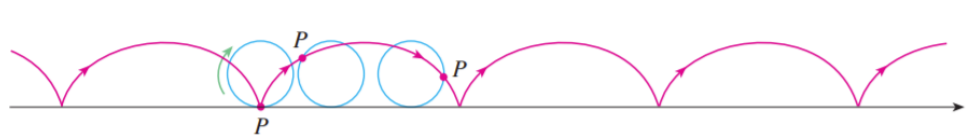
\includegraphics[width=0.95\linewidth]{res/Cycloid.png}
% \end{center}
% \end{frame}

% \begin{frame}{Polar Coordinates}
% We choose a point in the plane that is called the pole (or origin) and is
% labeled O. Then we draw a ray (half-line) starting at O called the polar
% axis. This axis is usually drawn horizontally to the right and corresponds
% to the positive x-axis in Cartesian coordinates.\\
% If P is any other point in the plane, let r be the distance from O to P and
% let $\theta$ be the angle (usually measured in radians) between the polar axis and the line OP as in Figure 1 . Then the point P is represented by the
% ordered pair $(r,\theta)$ and r,$\theta$ are called polar coordinates of P. We use the convention that an angle is positive if measured in the counterclockwise direction from the polar axis and negative in the clockwise direction. If P = O, then $r = 0$ and we agree that $(0,\theta)$ represents the pole for any value of $\theta$.
% \end{frame}
% \begin{frame}{Polar Coordinates}
% \begin{figure}[htb]
%   \centering
%   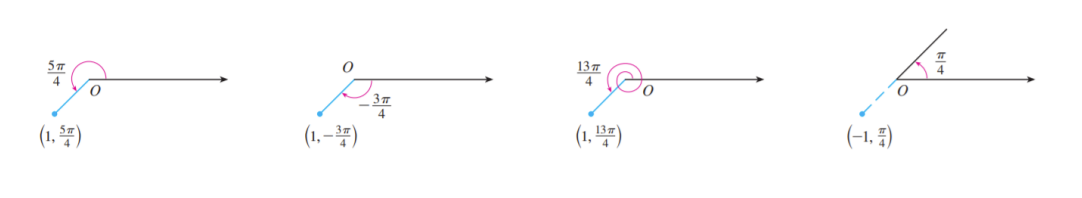
\includegraphics[width=0.95\linewidth]{res/polar.png}
% \end{figure}
% In fact, since a complete counterclockwise rotation is given by an angle
% $2\pi$, the point represented by polar coordinates $(r,\theta)$ is also represented by\\
% \begin{center}
%     $(r,\theta+2n\pi)$ and $(-r,\theta+(2n+1)\pi)$
% \end{center}
% \end{frame}

% \colortheme{blue!50!black}
% \begin{frame}{Polar Coordinates and Cartesian Coordinates}
% \begin{block}{Relationship between Polar Coordinates and Cartesian Coordinates}
%     \begin{center}
%         $x=r cos\theta$  $y=r sin \theta$\\
%         $r^2=x^2+y^2$  $tan\theta = \frac{y}{x}$
%     \end{center}
% \end{block}
% \end{frame}

% \colortheme{pink!100!black}
% \begin{frame}{Cartesian coordinates and Cylindrical coordinates}
%     \begin{block}{cylindrical to Cartesian coordinates}
%     \begin{center}
%         $x=r cos \phi$\\
%         $y=r sin \phi$\\
%         $z=z$
%     \end{center}
%     \end{block}
%     \begin{block}{inverse relations (from Cartesian to cylindrical coordinates) }
%     \begin{center}
%         $r=\sqrt{x^2+y^2}$\\
%         $tan \phi=\frac{y}{x}$\\
%         $z=z$
%     \end{center}
%     \end{block}
% \end{frame}

% \begin{frame}{Cartesian coordinates and Spherical coordinates}
%     \begin{block}{spherical to Cartesian coordinates}
%     \begin{center}
%         $x=r sin \theta cos \phi$\\
%         $y=r sin\theta sin \phi$\\
%         $z=r cos\theta$
%     \end{center}
%     \end{block}
%     \begin{block}{inverse relations (from Cartesian to spherical coordinates) }
%     \begin{center}
%         $r=\sqrt{x^2+y^2+z^2}$\\
%         $tan \phi=\frac{y}{x}$\\
%         $tan \theta=\frac{\sqrt{x^2+y^2}}{z}$
%     \end{center}
%     \end{block}
% \end{frame}

% \begin{frame}{Cardioid}
%     \begin{block}{Definition}
% - parametric representation:
% \begin{center}
%     $x(\theta)=2a(1-cos \theta)cos \theta$\\
%     $y(\theta)=2a(1-cos \theta)sin \theta$\\
%     $(0\leqslant \theta \leqslant 2\pi)$
% \end{center}
% - polar coordinates:
% \begin{center}
%     $r =2a(1-cos \theta)$\\
%     $(0\leqslant \theta \leqslant 2\pi)$
% \end{center}
% Cardioid is special Cycloid and special Limaçon
%     \end{block}
% \end{frame}

% \begin{frame}{Cardioid}
%     \begin{block}{Cardioid}
%         \begin{center}
%     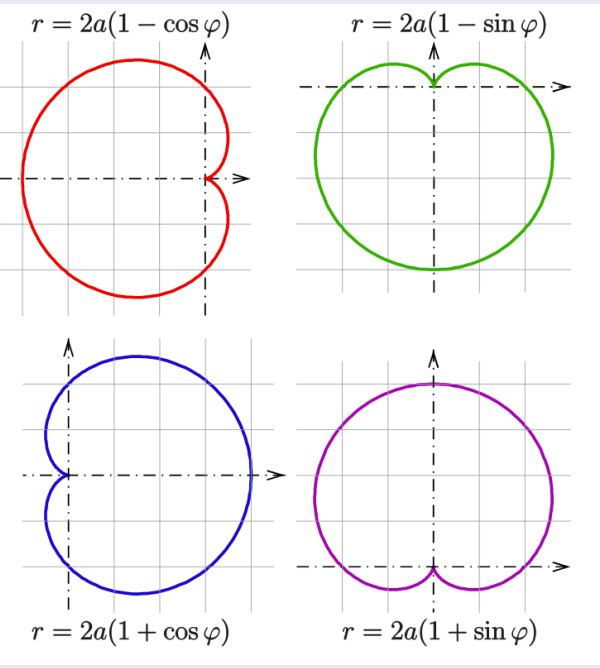
\includegraphics[width=0.5\linewidth]{res/Cardioid.png}
% \end{center}
%     \end{block}
% \end{frame}

% \begin{frame}{Limaçon}
%     \begin{block}{Definition}
%     \begin{center}
%         $r=1+c sin\theta$\\~\\
%         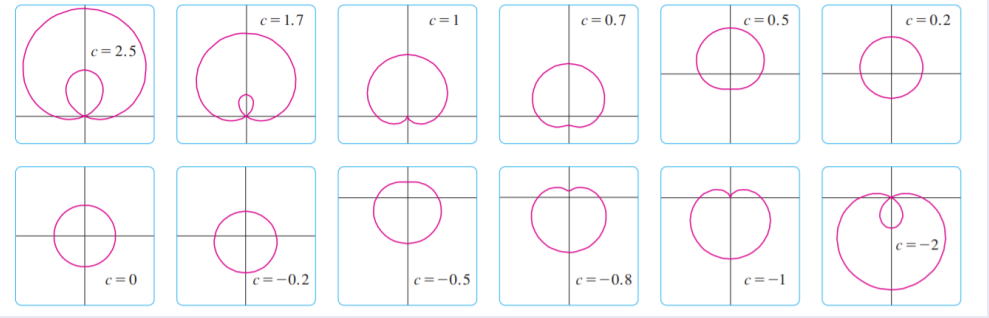
\includegraphics[width=0.85\linewidth]{res/limacon.png}
%     \end{center}
%     \end{block}
% \end{frame}
% \begin{frame}{Conchoid}
%     \begin{block}{Definition}
%     \begin{center}
%         $r=1+c sec\theta$\\~\\
%         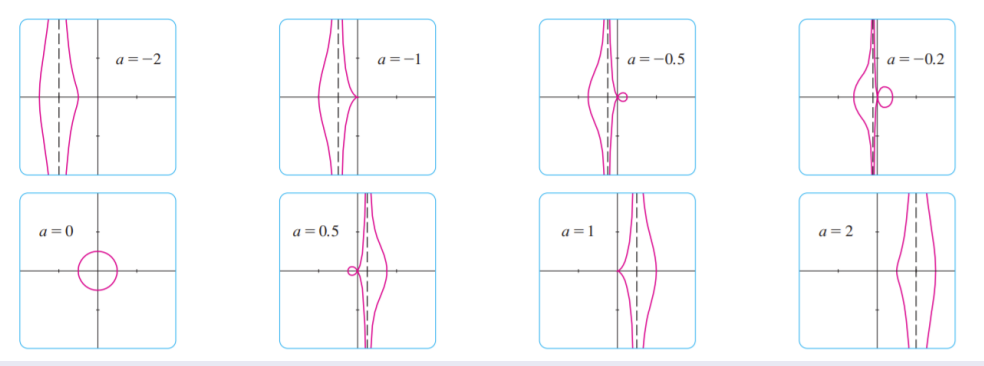
\includegraphics[width=0.85\linewidth]{res/Conchoid.png}
%     \end{center}
%     \end{block}
% \end{frame}
% \begin{frame}{Epicycloid}
%     \begin{block}{Definition}
%     \begin{center}
%         $x(\theta)=(R+r)cos\theta-r cos(\frac{R+r}{r}\theta)$\\
%         $y(\theta)=(R+r)sin\theta-r sin(\frac{R+r}{r}\theta)$\\~\\
%         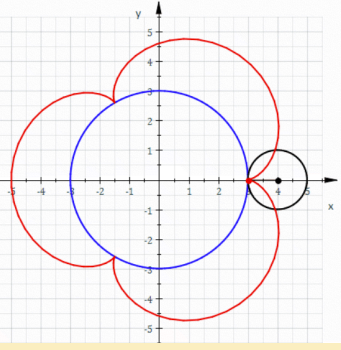
\includegraphics[width=0.55\linewidth]{res/Epicycloid.png}
%     \end{center}
%     \end{block}
% \end{frame}
% \begin{frame}{Epitrochoid}
%     \begin{block}{Definition}
%     \begin{center}
%         $x(\theta)=(R+r)cos\theta-d cos(\frac{R+r}{r}\theta)$\\
%         $y(\theta)=(R+r)sin\theta-d sin(\frac{R+r}{r}\theta)$\\~\\
%         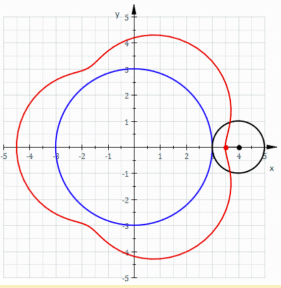
\includegraphics[width=0.55\linewidth]{res/Epitrochoid.png}
%     \end{center}
%     \end{block}
% \end{frame}
% \begin{frame}{Hypocycloid}
%     \begin{block}{Definition}
%     \begin{center}
%         $x(\theta)=(R-r)cos\theta-r cos(\frac{R-r}{r}\theta)$\\
%         $y(\theta)=(R-r)sin\theta-r sin(\frac{R-r}{r}\theta)$\\~\\
%         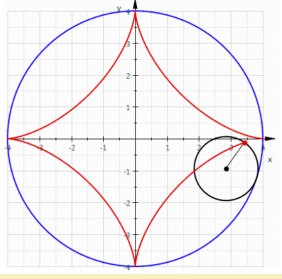
\includegraphics[width=0.55\linewidth]{res/Hypocycloid.png}
%     \end{center}
%     \end{block}
% \end{frame}
% \begin{frame}{Hypotrochoid}
%     \begin{block}{Definition}
%     \begin{center}
%         $x(\theta)=(R-r)cos\theta-d cos(\frac{R-r}{r}\theta)$\\
%         $y(\theta)=(R-r)sin\theta-d sin(\frac{R-r}{r}\theta)$\\~\\
%         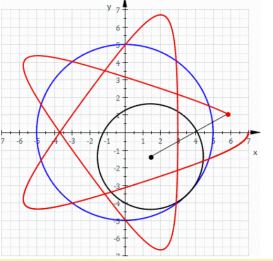
\includegraphics[width=0.55\linewidth]{res/Hypotrochoid.png}
%     \end{center}
%     \end{block}
% \end{frame}

% \begin{frame}{Bézier curves}
% \begin{block}{Definition}
% Bézier curves are used in computer-aided design and are named after the
% French mathematician Pierre Bézier (1910-1999), who worked in the
% automotive industry. A cubic Bézier curve is determined by four control
% points, $P_0 (x_0,y_0)$,$P_1 (x_1,y_1)$,$P_2 (x_2,y_2)$, and $P_3 (x_3,y_3)$, and is defined by the parametric equations:
% \begin{center}
%     $x=x_0 (1-t)^3 + 3x_1 t(1-t)^2 + 3x_2 t^2(1-t)+ x_3 t^3$\\
%     $y=y_0 (1-t)^3 + 3y_1 t(1-t)^2 + 3x_2 t^2(1-t)+ y_3 t^3$
% \end{center}
% \end{block}
% More Details: https://zhuanlan.zhihu.com/p/471457420
% \end{frame}

% \begin{frame}{Application of Bézier Curves in desmos}
%     \begin{center}
%     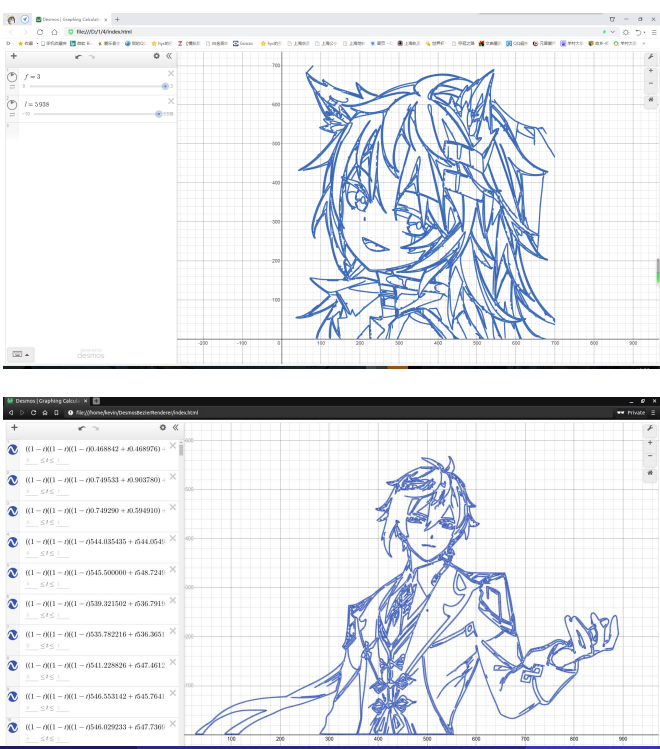
\includegraphics[width=0.6\linewidth]{res/demo1.png}
%     \end{center}
% \end{frame}
% \begin{frame}{Application of Bézier Curves in desmos}
%     \begin{center}
%     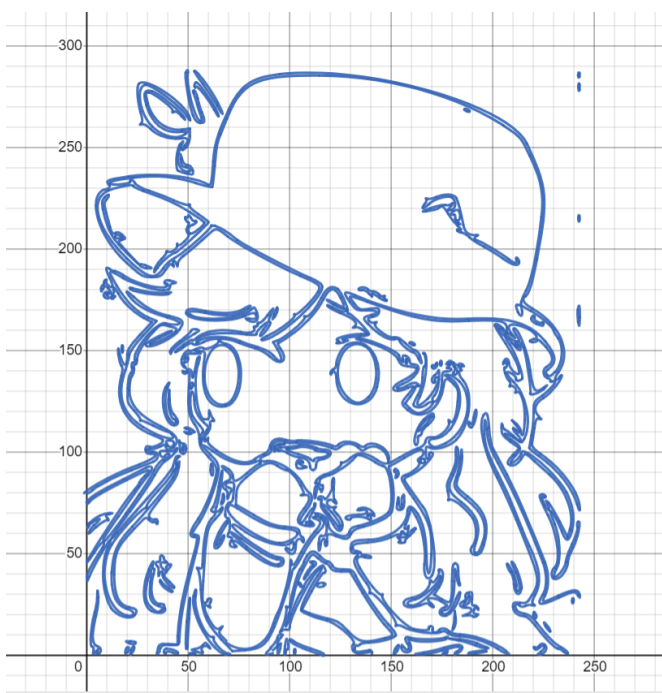
\includegraphics[width=0.6\linewidth]{res/demo2.png}
%     \end{center}
% \end{frame}
% \begin{frame}{Application of Bézier Curves in desmos}
%     \begin{center}
%     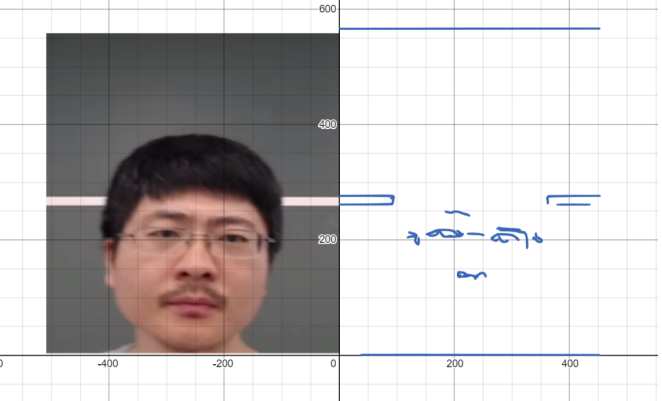
\includegraphics[width=0.75\linewidth]{res/demo.png}
%     \end{center}
% \end{frame}

% \colortheme{green!30!black}
% \begin{frame}{Tangents}
%     \begin{block}{Slope of the Tangent Line with Parametric Curves}
%     $$\frac{dy}{dx}=\frac{\frac{dy}{dt}}{\frac{dx}{dt}}$$
%     \end{block}
% For the second order derivative, we have:\\
% $$\frac{d^2y}{dx^2}=\frac{d}{dx}\frac{dy}{dx}=\frac{\frac{d}{dt}\frac{dy}{dx}}{\frac{dx}{dt}}$$
% \end{frame}

% \begin{frame}{Area and Arc Length}
%     \begin{block}{Area}
% We know that the area under a curve $y = F(x)$ from $a$ to $b$ is
% $A = \int_a ^b F(x) dx$, where $F(x) \geqslant 0$. If the curve is traced out once by the parametric equations $x = f(t)$ and $y = g(t)$, $\alpha \leqslant t \leqslant \beta$, then we can calculate an area formula by using the Substitution Rule for Definite Integrals as follows:
% $$A=\int _a^b y dx = \int_{\alpha}^{\beta} g(t) f^{\prime}(t) dt$$ or $$=\int^{\alpha}_{\beta} g(t) f^{\prime}(t) dt$$
%     \end{block}
% \end{frame}

% \begin{frame}{Arc Length}
%     \begin{block}{Arc Length}
%     If a curve C is described by the parametric equations $x = f(t)$,$y = g(t)$,$\alpha \leqslant t \leqslant \beta $, where $f^{\prime}$ and $g^{\prime}$ are continuous on $[\alpha,\beta]$ and C is traversed exactly once as t increases from$\alpha$ to $\beta$, then the length of C is
%     $$L=\int_{\alpha}^{\beta}\sqrt{(\frac{dx}{dt})^2+(\frac{dy}{dt})^2} dt $$
%     \end{block}
% \end{frame}

% \begin{frame}{Surface Area}
%     \begin{block}{Surface Area}
%         In the same way as for arc length, we can adapt to obtain a formula for
% surface area. If the curve given by the parametric equations $x = f(t)$,$y = g(t)$,$\alpha \leqslant t \leqslant \beta $ is rotated about the x-axis, where $f^{\prime}$ and $g^{\prime}$ are continuous and $g(t) \geqslant 0$, then the area of the resulting surface is given by
% $$ S=\int_{\alpha}^{\beta} 2\pi y\sqrt{(\frac{dx}{dt})^2+(\frac{dy}{dt})^2} dt $$
%     \end{block}
    
% \end{frame}

% \colortheme{blue!50!black}
% \begin{frame}{Tangents}
%     \begin{block}{Slope of the Tangent Line with  Polar Coordinates}
%     $$x=r cos\theta,y=r sin\theta$$
% where r can be regarded as a function of $\theta$. Hence we have
%     $$\frac{dy}{dx}=\frac{\frac{dy}{d\theta}}{\frac{dx}{d\theta}}=\frac{\frac{dy}{d\theta}sin \theta + r cos\theta}{\frac{dy}{d\theta} cos\theta -r sin\theta}$$
%     \end{block}
% \end{frame}
% \begin{frame}{Area And Arc Length}
%     Suppose we have the function in polar coordinates:
%     $$r=f(\theta),a \leqslant \theta \leqslant b$$
%     For the area enclosed by this function, we have:
%     $$A=\int_a^b \frac{1}{2}f^2(\theta)d\theta$$
%     For the area enclosed by this function, we have:
%     $$L=\int_a^b \sqrt{r^2+(\frac{dr}{d\theta})^2} d\theta$$
% \end{frame}

% \begin{frame}{Exercise 1}
%     \begin{block}{tangents}
%     Find equations of the tangents to the curve $x = 3t^2 +1, y = 2t^3 +1$ that
%     pass through the point $(4,3)$.
%     \end{block}
% \end{frame}

% \begin{frame}{Exercise 2}
% \begin{enumerate}
%         \item Find the exact length of the curve
%             \begin{center}
%                 $x=1+3t^2$, $y=4+2t^3$, $0 \leqslant t \leqslant 1$
%             \end{center}
%         \item
%             Find the area enclosed by the x-axis and the curve
%             \begin{center}
%                 $x=1+e^t$, $y=t-t^2$
%             \end{center}
%         \item
%            Find the exact area of the surface obtained by rotating the given curve about the x-axis.
%             \begin{center}
%                 $x=3t-t^3$, $y=3t^2$, $0 \leqslant t \leqslant 1$
%             \end{center}
%     \end{enumerate}
% \end{frame}

% \begin{frame}{Exercise 3 }
% \begin{enumerate}
%         \item Find the slope of the tangent line to the given polar curve at the point specified by the value of $\theta$
%             \begin{center}
%                 $r=2-sin\theta$, $\theta=\frac{\pi}{3}$
%             \end{center}
%         \item
%             Find the area of the region enclosed by one loop of the curve:
%             \begin{center}
%                 $r=2 sin5\theta$
%             \end{center}
%     \end{enumerate}
% \end{frame}

% \begin{frame}{Answers}
%     exercises 1:\\
%     $\frac{dy}{dx}=\frac{\frac{dy}{dt}}{\frac{dx}{dt}}=\frac{6t^2}{6t}=t$\\
%     when pass through $(4,3)$, we have $3-(2t^3+1)=t(4-(3t^2+1)) \Rightarrow t=1$ or $t=-2$\\
%     $\Rightarrow y=x-1$ or $y=-2x+11$\\
% \end{frame}
% \begin{frame}{Answers}
%     exercises 2:
%     \begin{enumerate}
%         \item
%             $L=\int_0^1\sqrt{(\frac{dy}{dt})^2+(\frac{dx}{dt})^2} dt=\int_0^1 6t \sqrt{1+t^2}dt = \int_1^2 \sqrt{u}(\frac{1}{2}d u)= 3 \cdot \frac{3}{2} [u ^ {\frac{3}{2}}]|_1^2= 2(2\sqrt{2}-1)$
%         \item
%              The curve $x = 1+e^t$,$y = t−t^2=t(1-t)$ intersects the x-axis when $y = 0$, that is, when $t = 0$ and $t = 1$. The corresponding values of x are $2$ and $1+e$. The shaded area is given by
%              $\int_2^{1+e} (y_T-y_B) dx = \int_0^1 (y(t)-0) x^{\prime}(t) dt=\int _0^1 (t-t^2)e^t dt $\\
%              $=\int _0^1 t e^t dt - \int_0^1 t^2 \cdot e^t dt$
%              $= 3\int_0^1 t e^t dt - t^2 e^t|_0^1$\\
%              $=3((t-1)e^t)|_0^1 - e =3-e$
%         \item
%             $x=3t-t^3$,$y=3t^2$,$0 \leqslant t \leqslant 1$.\\
%             $(\frac{dx}{dt})^2+(\frac{dy}{dt})^2=(3-3t^2)^2+(6t)^2=(3(1+t)^2)^2$\\
%             $S=\int_0^1 2\pi \cdot 3t^2 \cdot (1+t^2) dt$\\
%             $=18\pi(\frac{1}{3} t^3 + \frac{1}{5} t^5)|_0^1$\\
%             $=\frac{48}{5}\pi$
%     \end{enumerate}
% \end{frame}

% \begin{frame}{Answers}
%     \begin{enumerate}
%         \item 
%         $x=r cos\theta= (2-sin\theta)cos\theta$,$y=r sin\theta =(2-sin\theta) sin\theta$\\
%         $\frac{dy}{dx}=\frac{2cos\theta-sin2\theta}{-2sin\theta-cos2\theta}$\\
%         when $\theta = \frac{\pi}{3}$, $\frac{dy}{dx}=\frac{2-\sqrt{3}}{1-2\sqrt{3}}$
%         \item
%         $sin 5\theta= 0 \Rightarrow 5\theta=n\pi \Rightarrow \theta=\frac{\pi}{5} n$\\
%         $A=\int_0^{\frac{\pi}{5}} \frac{1}{2}(2sin5\theta)^2 d\theta$\\
%         $=2 \int_0^{\frac{\pi}{5}}\frac{1}{2}(1-cos10\theta)|_0^{\frac{\pi}{5}}=\frac{\pi}{5}$\\
%     \end{enumerate}
% \end{frame}

% \begin{frame}{Reference}
% [1] Huang, Jiahe. VV156\_RC4.pdf.2022.\\
% [2] Huang, Yucheng. VV156\_ RC6.pdf. 2021.\\
% [3] Chen, Jixiu et al. Mathematical Analysis (3rd Version). 2019\\
% [4] Li, Junhao.VV156\_RC5.pdf.2022.

% \end{frame}


% \colortheme{green!30!black}
% \section{Series}

% \begin{frame}{Limits of Sequences}
%     A sequence {$a_n$} has the limit L and we write:
%     \begin{center}
%     $ \mathop{lim} \limits_{n \rightarrow \infty} a_n = L$ or $a_n \rightarrow L$ as n $\rightarrow \infty$ 
%     \end{center}
%     if we can make the terms $a_n$ as close to L as we like by taking n sufficiently large. If $\mathop{lim} \limits_{n \rightarrow \infty} a_n$ exists, we say the sequence converges (or is convergent). Otherwise, we say the sequence diverges (or is divergent).
% \end{frame}


% \colortheme{blue!50!black}
% \begin{frame}{Limits of Sequences: Precise Definition}
% \begin{block}{Definition}
%     Suppose that there is a sequence $a_n$. If for any fixed positive number $\varepsilon$, there exits a positive integer N such that for any $n > N$, we have\\
%     $$|a_n - L|< \varepsilon$$\\
%     Then we say that the sequence an has the limit L.
% \end{block}
    
% \end{frame}
% \colortheme{green!30!black}
% \begin{frame}{Limits of Sequences}
%     \begin{block}{Theorems}
%         \begin{enumerate}
%             \item  If $lim_{n\rightarrrow \infty} f (x) = L$ and $f (n) = a_n$ when n is an integer, then $lim_{n\rightarrrow \infty} a_n = L$.
%             \item $lim_{n\rightarrow \infty} a_n = \infty$ means that for every positive number M there is an integer N such that if $n > N$ then $a_n > M$.
%             \item  (Squeeze theorem) If $a_n \leqslant b_n \leqslant c_n$ for $n \geqslant n_0$ and $lim_{n \rightarrow \infty} a_n = lim_{n \rightarrow \infty} c_n = L$, then $lim_{n\rightarrow\infty} b_n = L$.
%             \item If $lim_{n \rightarrow \infty} |a_n| = 0$, then $lim_{n \rightarrow \infty} a_n = 0$.
%             \item Every bounded, monotonic sequence is convergent.
%             \item *(Bolzano Weierstrass Theorem) A Bounded sequence must have a convergent subsequence.
%         \end{enumerate}
%     \end{block}
% \end{frame}
% \begin{frame}{Limits of Sequences}
%     \begin{block}{Properties}
%         If {$a_n$} and {$b_n$} are convergent sequences and c is a constant, then:
%         \begin{enumerate}
%         \item $\mathop{lim} \limits_{n \rightarrow \infty}(a_n+b_n)=\mathop{lim} \limits_{n \rightarrow \infty} a_n+ \mathop{lim} \limits_{n \rightarrow \infty}b_n$
%         \item $\mathop{lim} \limits_{n \rightarrow \infty}(a_n-b_n)=\mathop{lim} \limits_{n \rightarrow \infty} a_n- \mathop{lim} \limits_{n \rightarrow \infty}b_n$
%         \item $\mathop{lim} \limits_{n \rightarrow \infty} c a_n= c\mathop{lim} \limits_{n \rightarrow \infty} a_n$
%         \item $\mathop{lim} \limits_{n \rightarrow \infty}(a_n b_n)=\mathop{lim} \limits_{n \rightarrow \infty}a_n \cdot \mathop{lim} \limits_{n \rightarrow \infty} b_n$
%         \item $\mathop{lim} \limits_{n \rightarrow \infty}\frac{a_n}{b_n} =\frac{\mathop{lim} \limits_{n \rightarrow \infty} a_n}{\mathop{lim} \limits_{n \rightarrow \infty}b_n},(\mathop{lim} \limits_{n \rightarrow \infty}b_n \neq 0)$
%         \item $\mathop{lim} \limits_{n \rightarrow \infty} a_n ^p = (\mathop{lim} \limits_{n \rightarrow \infty} a_n)^p,(p>0, a_n>0)$
%         \end{enumerate}
%     \end{block}
% \end{frame}

% \begin{frame}{Series}
%     \begin{block}{Definition}
%         Given a series $\sum\limits_{n=1}^{\infty} a_n = a_1 + a_2 + ...$, let $s_n$ denote  its nth partial sum:\\
%         $$s_n=\sum\limits_{i=1}^{\infty} a_i = a_1 + a_2 + ...+a_n$$
%         If the sequence {$s_n$} is convergent and $\mathop{lim} \limits_{n \rightarrow \infty}  s_n = s$ exists as a real number, then the series $\sum a_n$ is called convergent and we write:\\
%         \begin{center}
%             $a_1+a_2+...+a_n=s$ or $\sum\limits_{i=1}^{\infty} a_i= s$
%         \end{center}
%         The number s is called the sum of the series. If the sequence {$s_n$} is divergent, then the series is called divergent.
%     \end{block}
% \end{frame}

% \begin{frame}{Geometric Series}
%     The geometric series:\\
%     $$\sum\limits_{n=1}^{\infty} ar^{n-1}=a+ar+ar^2+...$$
%     s convergent if $|r| < 1$ and its sum is\\
%     $$\sum\limits_{n=1}^{\infty} ar^{n-1} = \frac{a}{1-r}, |r|<1 $$
%     if If $|r| \geqslant 1$, the geometric series is divergent.
% \end{frame}
% \begin{frame}{P-Series}
%     \begin{block}{Definition}
%         P-series is defied as\\
%         $$\sum\limits_{n=1}^{\infty} \frac{1}{n^p}$$
%     \end{block}
%     If $p = 1$, then we also call it harmonic series:
%     $$\sum\limits_{n=1}^{\infty}\frac{1}{n} = 1 +\frac{1}{2}+\frac{1}{3}+\cdot\cdot\cdot$$
%     It is divergent.
% \end{frame}

% \colortheme{pink!100!black}
% \begin{frame}{Fourier Series}
%     \begin{block}{Definition}
%         $$s_N(x)=\frac{a_0}{2}+\sum\limits^{N}_{n=1}(a_n cos(\frac{2\pi nx}{P})+b_n sin(\frac{2\pi nx}{P}))$$
%     \end{block}
% \end{frame}

% \colortheme{blue!50!black}
% \begin{frame}{Fundamental Properties of Series}
%     \begin{block}{Requirement for Convergent Series}
%         Suppose the series $\sum_{n=1}^{\infty} x_n$ is convergent, then the sequence $x_n$ is an infinitesimal, which means
%         $$\mathop{lim} \limits_{n \rightarrow \infty} x_n = 0$$
%         This can be used to test if a series is divergent.
%     \end{block}
%     \begin{block}{Linearity for Convergent Series}
%     Suppose $\sum_{n=1}^{\infty} a_n = A$,$\sum_{n=1}^{\infty} b_n = B$, and $\alpha$,$\beta$ are two constants, then\\
%     $$\sum\limits_{n=1}^{\infty}(\alpha a_n + \beta b_n)= \alpha A + \beta B$$
%     \end{block}
% \end{frame}


% \begin{frame}{Several Methods}
%     \begin{enumerate}
%     \item Divergence Test Theorem (Requirement for Convergent Series)
%     \item Integral Test
%     \item Comparison Test
%     \item Cauchy Test (Root Test)
%     \item d’Alembert Test (Ratio Test)
%     \item Leibniz Test
%     \item Absolute Convergence Test
%     \end{enumerate}
% \end{frame}

% \begin{frame}{Integral Test}
%     Suppose f is a continuous, positive, decreasing function on $[1,\infty)$ and let $a_n = f (n)$. Then the series $\sum_1^{\infty} a_n$ an is convergent if and only if the improper integral \is convergent. In other words:\\
%     (i) If $\int_1^{\infty}f(x) dx$ is convergent, then $\sum_{n=1}^{\infty}a_n$ is convergent.
%     (ii) If $\int_1^{\infty}f(x) dx$ is divergent, then $\sum_{n=1}^{\infty}a_n$ is divergent.

% \end{frame}

% \begin{frame}{Integral Test: Important Conclusions for p-series}
% For what values of p is the series $\sum\limits_{n=1}^{\infty} \frac{1}{n^p}$ convergent?\\
% SOLUTION:\\
% (i) If $p<0$, then $lim_{n\rightarrow \infty}(\frac{1}{n^p})=\infty$\\
% (ii) If $p=0$ $lim_{n\rightarrow \infty}(\frac{1}{n^p})=1$\\
% In either case $lim_{n\rightarrow \infty}(\frac{1}{n^p}) \neq 0$\\
% (iii)$p>0$,$f(x)=\frac{1}{x^p}$ is clearly continuous, positive, and decreasing on $[1,\infty]$. And we have:
% $\int_1^{\infty} \frac{1}{x^p} dx $ converges if $p>1$ and diverges if $p \leqslant 1$
% \begin{block}{Conclusion}
% The p-series $\sum_{n=1}^{\infty}\frac{1}{n^p}$
% is convergent if $p>1$ and divergent if $p \geqslant 1$.
% \end{block}
% \end{frame}

% \begin{frame}{Comparison Test}
%     Suppose that $\sum a_n$ and $\sum b_n$ are series with positive terms.\\
% (i) If $\sum b_n$ is convergent and $a_n \leqslant b_n$ for all n, then $\sum a_n$ is also convergent.
% (ii) If $\sum b_n$ is divergent and $a_n \geqslant b_n$ for all n, then $\sum a_n$ is also divergent.
% In using the Comparison Test we must, of course, have some known series $\sum b_n$ for the purpose of comparison. Most of the time we use one of these
% series:\\
% - A p-series [$\sum \frac{1}{n^p}$ converges if $p > 1$ and diverges if $p \leqslant 1$]
% - A geometric series $\sum ar^{n-1}$ converges if $|r| < 1$ and diverges if $|r| \geqslant 1$]
% \end{frame}
% \begin{frame}{Comparison Test: Expressed by Limits}
%     \begin{block}{Theorem}
%         Suppose that $\sum a_n$ and $\sum b_n$ are series with positive terms. If
% $$\mathop{limits}\limits_{n \rightarrow \infty} \frac{a_n}{b_n}= c$$
% where c is a finite number and $c > 0$, then either both series converge or both diverge.
%     \end{block}
% Remark:Usually, this is more convenient to use.
% \end{frame}

% \begin{frame}{d’Alembert Test (Ratio Test)}
%     (i) If $lim_{n\rightarrow \infty}|\frac{a_{n+1}}{a_n}|=L<1$ then the series $\sum_{n=1}^{\infty} a_n$  is absolutely convergent (and therefore convergent).\\~\\
% (ii) If $lim_{n\rightarrow \infty}|\frac{a_{n+1}}{a_n}|=L>1$ or $lim_{n\rightarrow \infty}|\frac{a_{n+1}}{a_n}|=\infty$, then the series $\sum_{n=1}^{\infty}$ is divergent.\\~\\
% (iii) If $lim_{n\rightarrow \infty}|\frac{a_{n+1}}{a_n}|=L=1$, the Ratio Test is inconclusive; that is, no conclusion can be drawn about the convergence or divergence of $\sum a_n$.
% \end{frame}
% \begin{frame}{Cauchy Test (Root Test)}
%     (i) If $lim_{n \rightarrow \infty} \sqrt[n]{|a_n|} =L<1 $, then the series $\sum _{n=1}^{\infty} a_n$  is absolutely convergent (and therefore convergent).\\~\\
% (ii) If $lim_{n \rightarrow \infty} \sqrt[n]{|a_n|} =L>1 $ or $lim_{n \rightarrow \infty} \sqrt[n]{|a_n|} = \infty $, then the series $\sum _{n=1}^{\infty} a_n$ is divergent.\\~\\
% (iii) If $lim_{n \rightarrow \infty} \sqrt[n]{|a_n|} =L=1 $, the Root Test is inconclusive.
% \end{frame}

% \begin{frame}{Alternating Series}
%     \begin{block}{Definition}
%         If the series satisfies
% $$\sum\limits_{n=1}^{\infty}x_n=\sum\limits_{n=1}^{\infty}(-1)^{u+1} u_n$$
% Then we call it an alternating series.
%     \end{block}
% \end{frame}

% \begin{frame}{Leibniz Series}
%     Further, if the series
%     $$\sum\limits_{n=1}^{\infty}(-1)^{u+1} u_n$$
%     satisfies:
%     $(i) u_{n+1} \leqslant u_n$ for all n
%     $(ii) lim_{n\rightarrow \infty}u_n=0$
%     Then the series is convergent. \\
%     We call it Leibniz series.
% \end{frame}

% \begin{frame}{Important Conclusion}
%     \begin{block}{Conclusion}
%         The convergence and divergence property of a series has nothing to do with the first N terms, where N is a finite number.    
%     \end{block}
%     So, we can write:
%     $$\sum_{n=1}^{\infty}a_n= \sum_{n=1}^{N} a_n+ \sum _{n=N+1}^{\infty}$$
%     Then, if the series
%     $$\sum_{n=N+1}^{\infty} a_n$$
%     satisfies the conditions of Leibniz Series, we can still conclude that the series is convergent.
% \end{frame}

% \begin{frame}{Absolute Convergence and Conditional Convergence}
%     \begin{block}{Definition}
%         Suppose that $\sum\limits_{n=1}^{\infty} x_n$ is a convergent series. Then if $\sum\limits_{n=1}^{\infty} |x_n|$ is convergent, $\sum\limits_{n=1}^{\infty} x_n$ is absolutely convergent. Else $\sum\limits_{n=1}^{\infty} x_n$ is a conditionally convergent.
%     \end{block}
%     \begin{block}{Theorem}
%     If a series $\sum a_n$ is absolutely convergent, then it is convergent.
%     \end{block}
% \end{frame}

% \begin{frame}{Absolute Convergence and Conditional Convergence}
%     \begin{block}{Methods}
%     The convergence and divergence property of $\sum_{n=1}^{\infty} |x_n|$ can be determined by the criterion mentioned before.
%     \end{block}
%     Typically, if$\sum_{n=1}^{\infty} |x_n|$ diverges, $\sum_{n=1}^{\infty} x_n$ does not necessarily diverges. \\However, if the divergence property is determined by Ratio Test or Root Test, then the series$\sum_{n=1}^{\infty} x_n$ also diverges.That’s because these two criterion are based on the fact that the sequence is not approaches 0 $(x \rightarrow \infty)$.
% \end{frame}

% \begin{frame}{Shanks Transformation}
%     For each series $\sum_{n=0}^{\infty} a_n$, we can form the sequence of partial sums
%     $$A_n= \sum \limits _{k=0}^{n} a_n$$
%     and
%     $$S_n=\frac{A_{n+1}A_(n-1)-A_n^2}{A_{n+1}+A_{n-1}-2A_n}$$
%     This new sequence, called the Shanks transformation of the series, will usually converge faster than the original series. It is denoted by S ($A_n$), and works particular well on alternating series.
% \end{frame}
% \begin{frame}{Function Series}
%     Now let’s expand the concept of series to functions.
%     \begin{block}{Series with Function Terms}
%         Suppose un(x) is a function sequence with common domain E, then the sum of these infinite numbers of function terms $$u_1(x)+u_2(x)+\cdot+\cdot+\cdot+u_n(x)+\cdot+\cdot+\cdot$$ is called function series, denoted as $$\sum\limits_{n=1}^{\infty}u_n(x)$$
%     \end{block}
% \end{frame}

% \begin{frame}{Convergence Point and Convergence Domain}
%     Different from series of number terms, function series has the concept of convergence point and convergence domain.
%     \begin{block}{Convergence Point}
%         For a fixed $x_0 \in E$, if the series $$\sum\limits_{n=1}^{\infty}u_n(x_0)$$is convergent, then we say that the function series $$\sum\limits_{n=1}^{\infty}u_n(x)$$ is convergent at $x_0$.
%     \end{block}
% \end{frame}
% \begin{frame}{Convergence Point and Convergence Domain}
%     \begin{block}{Convergence Domain}
%     The set that includes all the convergence point of the given function series is called the convergence domain.
%     \end{block}
% \end{frame}
% \begin{frame}{Power Series}
%     Power Series is a special kind of function series.
%     \begin{block}
%     $$\sum\limits_{n=0}^{\infty} a_n(x-x_0)^n= a_0+ a_1 (x-x_0)+ a_2(x-x_0)^2 + ...+a_n(x-x_0)^n+...$$\\
%     This kind of function series is called power series.
%     \end{block}
    
% \end{frame}

% \begin{frame}{Radius of Convergence}
%     \begin{block}{Cauchy-Hadamard Theorem}
%     The power series $$\sum\limits_{n=0}^{\infty}a_n x^n$$
%     is absolutely convergent when $|x| < R$, and it is divergent when $|x| > R (R > 0)$. R is called the radius of convergence.
%     \end{block}
%     Note: at the endpoints $x=\pm R$, the convergence and divergence property of the function series should be judged by other methods.
% \end{frame}
% \begin{frame}{Radius of Convergence}
%     \begin{block}{Cauchy-Hadamard Theorem: for General Cases}
%     The power series $$\sum\limits_{n=0}^{\infty} a_n (x-x_0)^n$$
%     is absolutely convergent when $|x - x_0| < R$, and it is divergent when $|x - x_0| > R (R > 0)$.
%     \end{block}
% \end{frame}
% \begin{frame}{Radius of Convergence: Cauchy Test}
%     \begin{block}{Cauchy Test}
%     For the power series
% $$\sum\limits_{n=0}^{\infty}a_n x^n$$
% If
% $$\mathop{lim}\limits_{n\rightarrow \infty} \sqrt[n]{|a_n|}=A$$
% Then the radius of convergence of this power series is $\frac{1}{A}$
% Specially, If $A = 0$, then $R = +\infty$; if $A = +\infty$, then $R = 0$.
%     \end{block}
% \end{frame}
% \begin{frame}{Radius of Convergence: d’Alembert Test}
%     \begin{block}{d’Alembert Test}
%     For the power series
% $$\sum\limits_{n=0}^{\infty}a_n x^n$$
% If $$\mathop{lim}\limits_{n\rightarrow \infty} \frac{a_{n+1}}{a_n}=A$$
% Then the radius of convergence of this power series is $\frac{1}{A}$
% Specially, If $A = 0$, then $R = +\infty$; if $A = +\infty$, then $R = 0$.
%     \end{block}
% \end{frame}
% \begin{frame}{Properties of Power Series}
%     \begin{block}{Integrals Term by Term}
%     We can take the integrals of a power series term by term, if the interval lies in its domain of convergence.
%     \end{block}
% That means, if $a,b \in D $(D is the domain of convergence), then
% $$\int_a^b \sum\limits_{n=0}^{\infty} a_n x^n dx=\sum\limits_{n=0}^{\infty}\int_a^b a_n x^n dx$$
% If we take $a = 0$ and $b = x$, then
% $$\int_0^x \sum\limits_{n=0}^{\infty} a_n x^n dx=\sum\limits_{n=0}^{\infty}\frac {a_n}{n+1} x^{n+1} dx$$
% \end{frame}
% \begin{frame}{Properties of Power Series}
%     \begin{block}{ Derivatives Term by Term}
%     Suppose the power series $\sum_{n=0}^{\infty}a_n x^n$ has the radius of convergence R. Then we can take the derivatives term by term on $(−R,R)$.
%     \end{block}
%     $$\frac{d}{dx}\sum\limits_{n=0}^{\infty}a_n x^n = \sum\limits_{n=0}^{\infty} \frac{d}{dx} a_n x^n = \sum\limits_{n=0}^{\infty} n a_n x^{n-1}$$
%     $$\frac{d}{dx}\sum\limits_{n=0}^{\infty}a_n (x-x_0)^n = \sum\limits_{n=0}^{\infty} \frac{d}{dx} a_n (x-x_0)^n = \sum\limits_{n=0}^{\infty} n a_n (x-x_0)^{n-1}$$
% \end{frame}
% \begin{frame}{Shift the Index of Summation}
%    We can shift the ”starting point” of summation. General Case:
%    $$\sum\limits_{n=m}^{\infty} a_n (x-x_0)^n = \sum\limits_{n=m+k}^{\infty} a_{n-k} (x-x_0)^{n-k}$$
%    $$\sum\limits_{n=m}^{\infty} a_n (x-x_0)^n = \sum\limits_{n=m-k}^{\infty} a_{n+k} (x-x_0)^{n+k}$$
% \end{frame}
% \begin{frame}{Taylor Expansion of Elementary Functions}
%     $$e^x = \sum\limits_{n=0}^{\infty} \frac{x^n}{n!}=1+x+\frac{1}{2}x^3+\frac{1}{6}x^3+...,x \in R$$
%     $$ln(1+x)=\sum\limits_{n=0}^{\infty}\frac{(-1)^{n-1}}{n}x^n = x-\frac{x^2}{2}+\frac{x^3}{3}-..., x \in (-1,1]$$
%     $$sin x =\sum\limits_{n=0}^{\infty} \frac{(-1)^{n}}{(2n+1)!} x^{2n+1}=x -\frac{x^3}{3!} +\frac{x^5}{5!}-...,x\in R$$
%     $$cos x =\sum\limits_{n=0}^{\infty} \frac{(-1)^{2n}}{(2n)!}x^{2n} = 1 - \frac{x^2}{2}+ \frac{x^4}{4!}-...,x\in R$$
%     $$arctan x =\sum\limits_{n=0}^{\infty} \frac{(-1)^{n-1}}{2n-1}x^{2n-1} =x -\frac{x^3}{3}+\frac{x^5}{5}-..., x\in [-1,1]$$
% \end{frame}
% \begin{frame}{Taylor Expansion of Elementary Functions}
%     $$(1+x)^\alpha = \sum\limits_{n=0}^{\infty} \frac{(\alpha(\alpha-1)...(\alpha-n+1))}{n!} x^n$$
%     $$\frac{1}{1-x}=\sum\limits_{n=0}^{\infty} x^n = 1+x+x^2+...,x\in (-1,1)$$
%     $$\frac{1}{1-x}=\sum\limits_{n=0}^{\infty} (-1)^n x^n = 1-x+x^2-...,x\in (-1,1)$$
% \end{frame}

% \begin{frame}{Ex1}
%     \begin{block}{Sequences and Series}
%         Let $a_n=\frac{2n}{3n+1}$\\
%         1. Determine whether {$a_n$} is convergent.\\
%         2. Determine whether $\sum_{n=1}^{\infty} a_n$ is convergent.
%     \end{block}
% \end{frame}

% \begin{frame}{Ex2}
%     \begin{block}{Convergence and Divergence}
%     Find the values of x for which the series converges. Find the sum of
% the series for those values of x.\\
%         1. $$\sum\limits_{n=0}^{\infty}(-4)^n(x-5)^n$$
%         2. $$\sum\limits_{n=0}^{\infty}\frac{sin^n x}{3^n}$$
%     \end{block}
% \end{frame}
% \begin{frame}{Ex3: Integral Test}
%     \begin{block}{Determine whether the series is convergent or divergent}
%     1.$$\sum\limits_{n=1}^{\infty} \frac{n^2}{n^3+1}$$
%     2.$$\sum\limits_{n=1}^{\infty} \frac{n}{n^4+1}$$
%     \end{block}
% \end{frame}
% \begin{frame}{Ex4: Comparison Test}
%     \begin{block}{Determine whether the series is convergent or divergent}
%     1.$$\sum\limits_{n=1}^{\infty} \frac{1}{(n^2+2n+2)^2}$$
%     2.$$\sum\limits_{n=1}^{\infty} \frac{n!}{n^n}$$
%     \end{block}
% \end{frame}
% \begin{frame}{Ex5: Ratio \& Root}
%     \begin{block}{Determine whether the series is convergent or divergent}
%     1.$$\sum\limits_{n=1}^{\infty} \frac{n!}{n^n}$$
%     2.$$\sum\limits_{n=1}^{\infty} (\frac{-2n}{n+1})^{5n}$$
%     \end{block}
% \end{frame}
% \begin{frame}{Ex6}
%     1. Determine the Power Series Expansion of $f (x) = \frac{1}{3+5x-2x^2}$
% at $x = 0$.\\
% 2. Determine the Power Series Expansion of $f (x) = ln (\frac{sinx}{x})$
% at $x = 0$.
% \end{frame}
% \colortheme{green!30!black}
% \section{Differential Equation}

% \begin{frame}{Differential Equation}
%     \begin{block}{Definition}
%         Equations representing the relationship between some unknown functions, the derivative of those functions and the independent variable.
        
%         \textbf{Order}: The order of the highest derivative of the unknown function is called the order of the differential equation.
        
%         \textbf{Linear}: The highest degree of the unknown function and its derivatives of any order is 1.
        
%         Generally, $n^th$ order differential equations have the form of $F(x, y, y', ....., y^{(n)}) = 0$
%     \end{block}
%     In Vv156, we only need to solve some special types of ODEs.
% \end{frame}


% \subsection {Type 1}
% \begin{frame}{Type 1:  y' + p(x) y = q(x) }
% Step1: Find the general solution to the corresponding homogeneous ode $y' + p(x)y = 0$
    
%    \centering
%     $\dfrac{dy}{dx} = -p(x) y$    
        
%     $\dfrac{dy}{y} = -p(x)dx$

%     $ln|y| = -\int p(x)dx + c_1$
    
%     $y_g = C e^{-\int p(x)dx} (C = e^{\pm c_1})$

% \end{frame}

% \begin{frame}{Type 1:$y' + p(x) y = q(x)$}

% Step2: Find one special solution to $y' + p(x) y = q(x)$

% \centering
% Variation of constants: 

% $Ce^{-\int p(x)dx} \rightarrow C(x)e^{-\int p(x)dx}$

% $y' = C'(x)e^{-\int p(x)dx} - C(x)p(x) e^{-\int p(x)dx}$

% $C'(x)e^{-\int p(x)dx} - C(x)p(x) e^{-\int p(x)dx} + C(x)p(x)e^{\int p(x)dx} = q(x)$

% $C'(x)e^{-\int p(x)dx} = q(x)$

% $C'(x) = q(x)e^{\int p(x)dx}$

% $C(x) = \int q(x)e^{\int p(x)dx} dx + C_2$

% Since we only need to find one special solution, we assume $C_2 = 0$

% $y_s = e^{-\int p(x)dx}\cdot \int q(x)e^{p(x)dx} dx$
% \end{frame}



% \begin{frame}{Type 1:$y' + p(x) y = q(x)$}
%     Step 3: Combine $y_g$ and $y_s$ together
% \begin{equation*}
%     y = Ce^{-\int p(x)dx} + e^{-\int p(x)dx}\cdot \int q(x)e^{p(x)dx} dx
% \end{equation*}
% \end{frame}

% \begin{frame}{Bernoulli's equation}
% \begin{block}{$y' + p(x)y = q(x) y^n$}
% When $n\pm 0, 1$ the equation is not linear.

% However, we can do some transformation:
% \begin{enumerate}
%     \item $y^{-n}\cdot y' + p(x) \cdot y^{1-n} = q(x)$
%     \item $z = y^{1-n}$
% \end{enumerate}
%     Then, $\dfrac{dz}{dx} = (1-n)y^{-n}\dfrac{dy}{dx}$
    
%     Thus, $z' + (1-n)p(x) z = (1-n)q(x)$
    
%     which is in the form of $y' + p(x)y = q(x)$
% \end{block}
    
% \end{frame}

% \subsection{Type 2}

% \begin{frame}{Type 2: $y'' + py' + qy = f(x)$}
% Step 1: Find the general solution to the corresponding homogeneous ode $y'' + py' + qy = 0$
%     Solve the characteristic equation: $\lambda^2 + p\lambda + q = 0$
%     \begin{equation*}
%         \left\{
%         \begin{aligned}
%         &\text{Two different real roots} \ \lambda_1, \lambda_2 \quad y_g = C_1 e^{\lambda_1 x} + C_2 e^{\lambda_2 x}\\
%         & \text{Two equal real roots} \ \lambda \quad y_g = C_1 e^{\lambda x} + C_2 xe^{\lambda x}\\
%         & \text{Two different complex roots} \ \alpha\pm \beta i \quad y_g = C_1 e^{\alpha x}sin\beta x + C_2 e^{\alpha x}cos\beta x
%         \end{aligned}
%         \right.
%     \end{equation*}
    
% \end{frame}

% \begin{frame}{Type 2: $y'' + py' + qy = f(x)$}
%     Step 2: Find one special solution to $y'' + py' + qy = f(x)$ 
    
%     In Vv156, we only have two types of $f(x)$:
%     \begin{enumerate}
%         \item $f(x) = e^{\lambda x}P_m(x)$
%         \item $f(x) = e^{\lambda x}[P_n(x)cos(\omega x) + P_l(x) sin(\omega x)]$
%     \end{enumerate}
%     For both 1, 2, we first need to check whether $\lambda (\pm \omega i)$ is the root of the characteristic equation $\lambda^2 + p \lambda + q = 0$ or not
    
    
    
% \end{frame}

% \begin{frame}{Type 2: $y'' + py' + qy = f(x)$}
% \textbf{$f(x) = e^{\lambda x}P_m(x)$:}
% \begin{table}[!ht]
%             \centering
%             \begin{tabular}{c|c}
                 
%                  $1$  & $k$ \\
                 
%                  \hline
%                  \makecell{$\lambda$ is one of the different real\\ roots of $\lambda^2 + p\lambda + q = 0$}
%                  & $1$\\
                 
                 
                 
%                  \hline
%                 \makecell{$\lambda$ is the identical real \\roots of $\lambda^2 + p\lambda + q = 0$}
%                  & $2$\\
                 
%                  \hline
%                  \makecell{$\lambda$ is not the real\\ root of $\lambda^2 + p\lambda + q = 0$}
%                  & $0$
                 
%             \end{tabular}
%     \end{table}
% \textbf{$f(x) = e^{\lambda x}[P_n(x)cos(\omega x) + P_l(x) sin(\omega x)]$:}   
%     \begin{table}[!ht]
%             \centering
%             \begin{tabular}{c|c}
                 
%                  $2$  & $k$ \\
                 
%                  \hline
%                  \makecell{ $\lambda \pm \omega i$ are the complex\\ roots of $\lambda^2 + p\lambda + q = 0$ }
%                  & $1$\\
                 
                 
                 
                 
                 
%                  \hline
%                  \makecell{$\lambda \pm \omega i$ are not the complex\\ roots of $\lambda^2 + p\lambda + q = 0$} 
%                  & $0$
                 
%             \end{tabular}
%     \end{table}
% \end{frame}

% \begin{frame}{Type 2: $y'' + py' + qy = f(x)$}
% Apply undetermined coefficient method:
% \begin{itemize}
%     \item For 1: $y_s = x^k e^{\lambda x}\cdot Q_m(x) $
%     \item For 2: $y_s = x^k e^{\lambda x}[Q_m(x)cos(\omega x) + R_m(x) sin(\omega x)]$\  
%     $(m = MAX\{n ,l\})$
% \end{itemize}
% $Q_m$ and $R_m$ are another polynomial of degree m

% $\rightarrow$ Calculate $y'_s$ and $y''_s$ to solve $Q_m$ and $R_m$
    
% \end{frame}

% \begin{frame}{Type 2: $y'' + py' + qy = f(x)$}
%     Step 3: Combine $y_g$ and $y_s$ together
    
%     If $f(x) = f_1(x) + ... + f_n(x)$, and $f_i(x)$ is the form of 1, 2, we can calculate $y_{si}$ separately.
% \end{frame}

% \begin{frame}{Exercise}
%     \begin{enumerate}
%         \item $y' = \dfrac{y}{2x} + \dfrac{x^2}{2y}$
%         \item $y'' + 6y' + 10y = e^{-3x}sinx$
%     \end{enumerate}
% \end{frame}

% \begin{frame}{Exercise}
%     Solution 1:
    
%     \begin{enumerate}
%         \item $y' + (-\dfrac{1}{2x})y = 0.5x^2y^{-1}$\\
%         $yy' + (-\dfrac{1}{2x})y^2 = 0.5 x^2$
%         \item Let $z = y^2$ \rightarrow $\dfrac{dz}{dx} = 2y \dfrac{dy}{dx}$\\ $z' - \dfrac{z}{x} = x^2$\\Now $p(x) = -\dfrac{1}{x}$ $q(x) = x^2$
%         \item Apply $y = Ce^{-\int p(x)dx} + e^{-\int p(x)dx}\cdot \int q(x)e^{p(x)dx} dx$ \\We can get $z = Cx + \dfrac{1}{2}x^3$\\Thus, $y = \pm \sqrt{Cx + \dfrac{1}{2}x^3}$
        
%     \end{enumerate}
% \end{frame}

% \begin{frame}{Exercise}
% Solution 2:
% \begin{enumerate}
%     \item $\lambda^2 + 6\lambda + 10 = 0$ \ $\lambda = -3 \pm i$ \\Thus, the general solution is $y_g = e^{-3x}(C_1cosx + C_2 sinx)$
%     \item Observe $e^{-3x}sinx$ \rightarrow $\lambda = -3, \omega = 1$ \\ Since $-3\pm i$ are complex roots of $\lambda^2 + 6 \lambda + 10 = 0$, there is k = 1 \\So $y_s = e^{-3x}x(acosx + bsinx)$\\ $y'_s = e^{-3x}x[(b-3a)cosx + (-3b-a)sinx] +e^{-3x}(acosx + bsinx)$\\
%     $y''_s = e^{-3x}x[(8a - 6b)cosx + (6a + 8b)sinx] + e^{-3x}[(2b-6a)cosx - (2a + 6b)sinx]$\\
%     Since $y''+6y'+ 10y = e^{-3x}sinx$\\ Check the coefficient, $a = -0.5, b = 0$\\ $y_s = e^{-3x}x (-0.5cosx)$
%     \item Combine $y_g$ and $y_s$\\
%     $y = y_g + y_s = C_1 e^{-3x}cosx + C_2 e^{-3x}sinx - 0.5 xe^{-3x}cosx$

% \end{enumerate}
% \end{frame}
\thankframe



\end{document}
